\documentclass[9pt, a4paper]{extarticle}
\usepackage{amsmath,amssymb}
\usepackage{graphicx}
\usepackage{hyperref}
\usepackage{mathpazo}
\usepackage{microtype}
\usepackage{booktabs}
\usepackage[left=1in, right=1in, top=0.7in, bottom=0.7in]{geometry}
\usepackage{parskip}
\usepackage{enumitem}
\setlist{nosep}
\usepackage[font=footnotesize,labelfont=bf,skip=2pt]{caption}
\usepackage{titlesec}
% \titlespacing*{\section}{0pt}{0.5em}{4pt}
% \titlespacing*{\subsection}{0pt}{0.4em}{2pt}
\usepackage{verbatim}
\usepackage{fancyvrb}
\RecustomVerbatimEnvironment{verbatim}{Verbatim}{fontsize=\footnotesize}
\usepackage{algorithm}
\usepackage{algpseudocode}
\captionsetup[algorithm]{font=footnotesize,labelfont=bf,skip=2pt}
\usepackage{tikz}
\usetikzlibrary{arrows.meta, positioning, fit, backgrounds, automata, decorations.pathreplacing, shapes.geometric}
\usepackage{tikz-timing}

\newcommand{\strutrow}{\rule{0pt}{2.2ex}}

\hypersetup{
    colorlinks=true,
    linkcolor=blue,
    citecolor=blue,
    urlcolor=blue
}

\title{GB3 RISC-V: Processor Architecture and Optimizations}
\date{}

\raggedbottom
\setlength{\floatsep}{8pt plus 2pt minus 2pt}
\setlength{\textfloatsep}{10pt plus 2pt minus 2pt}
\setlength{\intextsep}{8pt plus 2pt minus 2pt}

\begin{document}
\maketitle

\section{Introduction}

This document is a technical reference for the GB3 RISC-V project, covering the iCE40UP5K FPGA platform, the picorv32 processor and PicoSoC, and background on the design of microarchitecture. It condenses the core content of Harris~\cite{harris2022} (Chapters 2--5) and Patterson~\cite{patterson2017} alongside analysis of the picorv32 microarchitecture.

\begin{comment}
This article is a design document laying out design approach to improve a RISC-V processor
I have knowledge of verilog, boolean algebra, combinational and sequential circuits (MUX, decoders, FFs, ROM, PLA PAL etc)
But extremely minimal knowledge of computer, processor, systolic array architecture

This article will build up the background behind core ideas in digital design/computer architecture, while exploring a concrete hardware iCEBreaker and a concrete processor the picorv32 to illustrate these concepts. Its important to explain these architecture concepts clearly with relevant diagrams, pretty much a condensed version of the books below.

I have 2 textbooks - which their Table-Of-Contents are availaible - Harris Digital Design Comp Arch (RISCV Edition) and Patrick Hennessy Comp Arch (RISCV Edition)

Throughout this document, you will be using tikz diagrams, alongside screenshots of the abovementioned textbook
, as well as screenshots of any processor manuals and/or diagrams to illustrate concepts.
Before writing any section or subsection, you should always write the scaffolding first and let me approve it. then you will directly read the chapters of those books and any core data sheet, which will act as crucial context for the design doc

I want as much of the core content of the textbook as possible integrated into this document, as it also functions as a condensed mini textbook of Harris chapters (6-9) for myself. (I'm already familiar with digital logic, combinational and sequential logic, arithmetic circuits, PLA/FPGA/ROM, verilog etc)

The scaffolding comment blocks are important, these are to see what content to integrate into these sections, and which sections of the book to reference. When I ask you to update the scaffolding blocks, try not to delete existing lines, but instead integrate new content into the existing structure. That is, there is good reason to delete things and restructure, which of course I am happy to do, but stop and let me know of this.
There should not need to be WRITTEN and READ etc status symbols, these should be immediately obvious from readintg the scaffolding and existing content

FORMATTING CONVENTIONS:
  \textbf{bold}   — core named concepts on first introduction (e.g. architectural state, forwarding, Hazard Unit).
                    Use sparingly; once a term is introduced bold, subsequent uses are plain text.
                    
                    these strucural convention which is diff from inline stuff etc
                    - fine to use for bullet point naming too.
                    - fine to use for paragraph start etc
  \textit{italic} — secondary emphasis, less critical terms, or English-word emphasis (e.g. stall, bubble, flush).
  \texttt{mono}   — anything that is code, a signal name, a register name, or a Verilog identifier
                    (e.g. \texttt{mem\_valid}, \texttt{reg\_op1}, \texttt{cpu\_state}).
                    try not to italicise signal/register names; always use \texttt{}.
\end{comment}

\section{Processor Architecture}

\begin{comment}
Overall chapter reading order for deep-dive:
  Harris Ch 6 (Architecture) -> Ch 7 (Microarchitecture) -> Ch 8.1--8.3 (Memory hierarchy, caches) -> Ch 9.2 (Memory-mapped I/O)
  Patterson Ch 2 (Instructions) -> Ch 4 (The Processor)
  Source: picorv32.v, picosoc/picosoc.v, picosoc/icebreaker.v
\end{comment}

A processor executes a program by repeatedly performing the same loop: \textbf{fetch} an instruction from memory, \textbf{decode} it to determine what operation to perform, \textbf{execute} the operation, and \textbf{write back} the result. Understanding a processor requires separating two levels of abstraction:

\begin{itemize}
    \item The \textbf{instruction set architecture (ISA)} is the programmer's contract with the hardware. It defines the set of instructions the processor understands \textit{(instruction set)}, the registers available, how memory is addressed, and how instructions are encoded as binary \textit{(instruction format)}. Multiple chips can implement the same ISA.

    \item The \textbf{microarchitecture} is the hardware implementation of the ISA. It determines \emph{how} each instruction is executed: how many clock cycles it takes, how the datapath is organised (ALU, register file, memory interface), and how the control logic sequences the operations. The same ISA can be implemented as a single-cycle, multicycle, or pipelined microarchitecture, each with different trade-offs in speed, area, and power.
\end{itemize}

RISC-V is an ISA, and the picorv32 is one microarchitecture that implements it. The next few sections condenses the Harris \cite{harris2022} textbook, where Section~\ref{sec:isa} covers the ISA (Harris Chapter~6); Section~\ref{sec:microarch} covers the microarchitecture (Harris Chapter~7) and Section~\ref{sec:memory} covers memory systems (Harris Chapter~8).

\section{RV32I Instruction Set Architecture}
\label{sec:isa}

 RISC-V ISA is motivated by four design principles articulated by Patterson and Hennessy:

\begin{enumerate}
    \item \textbf{Regularity supports simplicity.} A consistent instruction format --- same number of operands, same field positions --- simplifies the decoder hardware. This is why every RV32I instruction is 32~bits, \texttt{opcode} is always at [6:0], \texttt{rs1} always at [19:15], and so on.
    \item \textbf{Make the common case fast.} Keep the instruction set small so that each instruction can be decoded and executed quickly. Complex operations (e.g.\ string copy) are built from sequences of simple instructions, rather than adding slow, seldom-used complex instructions.
    \item \textbf{Smaller is faster.} Fewer registers mean shorter addresses and faster access. 32~registers is a sweet spot: enough to avoid excessive spilling to memory, few enough that each register address fits in 5~bits.
    \item \textbf{Good design demands good compromises.} A single instruction format would be simplest but too restrictive; many formats would be flexible but hard to decode. RISC-V compromises with four main formats (R, I, S/B, U/J), balancing regularity with expressiveness.
\end{enumerate}

For reference tables of RISC-V compressed instructions, register names, instruction formats etc refer to the first few pages of \cite{harris2022}.

\begin{comment}
READ: Harris §6.1--6.2 (intro, registers, memory, constants)
READ: Harris §6.4.1--6.4.5 (instruction formats R/I/S/B/U/J, immediate encodings)
READ: Patterson §2.5 (Representing Instructions in the Computer)

FIGURES TO SCREENSHOT:
  - Harris Table 6.1 (p.305) --- register set names/numbers/conventions
  - Harris Figure 6.27 (p.340) --- immediate encoding consistency across all formats
  - Patterson Figure 2.5 (p.91) --- RISC-V instruction encoding table (opcode/funct3/funct7 for each instruction)

CUSTOM TIKZ DIAGRAMS:
  - Unified instruction format bit-field diagram: all 6 types (R/I/S/B/U/J) stacked, with bit positions and field names, highlighting that opcode[6:0] is always in the same place, rs1 is always [19:15], etc.

CONTENT (follows Harris Ch 6 structure: §6.2 assembly → §6.3 programming → §6.4 machine language → §6.5--6.7 system):

  §6.2 Assembly Language:
  1. Assembly language and machine language intro (§6.2.1): add example, binary encoding preview
  2. Registers (§6.2.2, Harris Table 6.1): x0--x31, naming conventions, callee/caller-saved
  3. Memory model (§6.2.2, §6.6.1): byte-addressable, little-endian, load-store architecture
     Addressing modes (§6.4.6): register, immediate, base (lw/sw offset), PC-relative (branches/jal/auipc)

  §6.3 Programming (comprehensive condenser → §4.4 Programming Model):
  4. Program flow and the PC (§6.3.1): instructions at sequential addresses (+4), PC tracks current
  5. Logical, shift, multiply (§6.3.2): and/or/xor, sll/srl/sra (R and I forms), slli for array indexing
  6. Branching and conditionals (§6.3.3--6.3.4): 6 branch instructions, opposite-condition pattern,
     if/else assembly example, switch/case = chain of bne
  7. Loops (§6.3.5): while (test opposite at top), do/while (test same at bottom), for (= while + init + incr)
  8. Arrays (§6.3.6): base + 4i pattern, slli+add+lw, byte/halfword arrays (lb/sb, no scaling)
  9. Function calls and the stack (§6.3.7): jal/jalr, a0--a7 args, push/pop pattern,
     preserved vs nonpreserved (Harris Table 6.3), leaf vs nonleaf, recursive, stack frame diagram
  10. Pseudoinstructions (§6.3.8, Harris Table 6.4): j, ret, mv, li, call, nop, not

  §6.4 Machine Language:
  7. Instruction formats (§6.4.1--6.4.4): R/I/S/B/U/J as unified TikZ figure
     Key insight: opcode[6:0] determines format, funct3 refines op, funct7 bit 5 distinguishes add/sub
  8. Instruction classes table with opcodes and operations + datapath usage TikZ diagram
  9. Immediate encoding (§6.4.5): sign bit always at instr[31], bit-field regularity (Harris Figure 6.27)
  10. Building 32-bit constants (§6.4.4): lui + addi trick, bit-11 sign-extension correction

  §6.5--6.7 System:
  11. Memory map and stored program (§6.4.8, §6.5.1, Harris Figure 6.31)
  12. Signed/unsigned variants (§6.6.3): slt/sltu, blt/bltu, lb/lbu, mul/mulhu, div/divu
  13. Exceptions and privilege levels (§6.6.2, Harris Table 6.6): U/S/M modes, CSRs, mret
  14. Extensions + picorv32 subset (§6.6.5, §6.7.1): merged table with picorv32 column; M via PCPI, C details

NOT INCLUDED:
  - §6.8 x86 comparison
\end{comment}

\subsection{Assembly Language and Machine Language}

A programmer might write instructions in \textbf{assembly language}, a human-readable notation where each line specifies an operation (e.g. \texttt{add}) and its operands (usually data stored in registers, memory, or explicitly encoded in the instruction itself):

\begin{center}\ttfamily\small
add s2, s3, s4 \quad\textrm{\normalfont\scriptsize\color{gray}(add contents of registers s3 and s4, store result in s2)}
\end{center}

The assembler translates each instruction into \textbf{machine language} --- the 32-bit binary word the hardware actually fetches and decodes. Each field in the binary word encodes a specific piece of information:

\begin{center}\small
\begin{tabular}{@{}c c c c c c l@{}}
    \toprule
    \texttt{funct7} & \texttt{rs2} & \texttt{rs1} & \texttt{funct3} & \texttt{rd} & \texttt{opcode} & \\
    \midrule
    \texttt{0000000} & \texttt{10100} & \texttt{10011} & \texttt{000} & \texttt{10010} & \texttt{0110011} & = \texttt{0x01498933} \\
    \scriptsize 7 bits & \scriptsize s4 (x20) & \scriptsize s3 (x19) & \scriptsize add & \scriptsize s2 (x18) & \scriptsize R-type ALU & \\
    \bottomrule
\end{tabular}
\end{center}

The processor never sees the text ``\texttt{add s2, s3, s4}'' --- it sees only the 32-bit number \texttt{0x01498933} fetched from instruction memory. The structure of these 32-bit words is defined by the \emph{instruction formats}.

\subsection{RISC-V Registers}

The RISC-V ISA defines a \textbf{32-bit architectural state}: \textbf{32 general-purpose registers} \texttt{x0}--\texttt{x31} and a program counter (PC). Register \texttt{x0} is hardwired to zero; writes to it are discarded. This constraint simplifies the ISA --- pseudo-instructions like \texttt{nop} (= \texttt{addi x0, x0, 0}) and \texttt{mv} (= \texttt{addi rd, rs1, 0}) fall out naturally.

\begin{table}[htbp]
\centering\small
\begin{tabular}{@{}l l l l@{}}
    \toprule
    Name & Reg & Use & Preserved? \\
    \midrule
    \texttt{zero} & \texttt{x0} & Constant 0 & --- \\
    \texttt{ra} & \texttt{x1} & Return address & Callee \\
    \texttt{sp} & \texttt{x2} & Stack pointer & Callee \\
    \texttt{gp} & \texttt{x3} & Global pointer & --- \\
    \texttt{tp} & \texttt{x4} & Thread pointer & --- \\
    \texttt{t0}--\texttt{t2} & \texttt{x5}--\texttt{x7} & Temporaries & Caller \\
    \texttt{s0}/\texttt{fp} & \texttt{x8} & Saved / frame pointer & Callee \\
    \texttt{s1} & \texttt{x9} & Saved & Callee \\
    \texttt{a0}--\texttt{a1} & \texttt{x10}--\texttt{x11} & Args / return values & Caller \\
    \texttt{a2}--\texttt{a7} & \texttt{x12}--\texttt{x17} & Arguments & Caller \\
    \texttt{s2}--\texttt{s11} & \texttt{x18}--\texttt{x27} & Saved & Callee \\
    \texttt{t3}--\texttt{t6} & \texttt{x28}--\texttt{x31} & Temporaries & Caller \\
    \bottomrule
\end{tabular}
\caption{RV32I register naming conventions and usage. ``Callee'' = must be saved/restored by called function; ``Caller'' = may be clobbered by any call.}
\label{tab:rv32-regs}
\end{table}

\subsection{RISC-V Memory model and Addressing modes}

To address the data stored in memory, RISC-V uses a \textbf{byte-addressable} (each byte is mapped to unique address), \textbf{little-endian} (address is LSB) memory space with 32-bit addresses ($2^{32} = 4$\,GB). Each 32 bit word consists of four 8-bit bytes, so each word address also has 32 bits, and are multiples of 4. All data transfer between registers and memory goes through explicit load/store instructions --- there are no memory operands in ALU instructions (this is the defining feature of a \emph{load-store architecture}). Instructions can only operate on registers, not directly on memory. Figure~\ref{fig:mem-layout} shows how bytes and words are arranged. Each word occupies 4 consecutive byte addresses; the word address is the address of its lowest byte \footnote{RISC-V is little-endian, so the least significant byte is at the lowest address}

\begin{figure}[htbp]
    \centering
    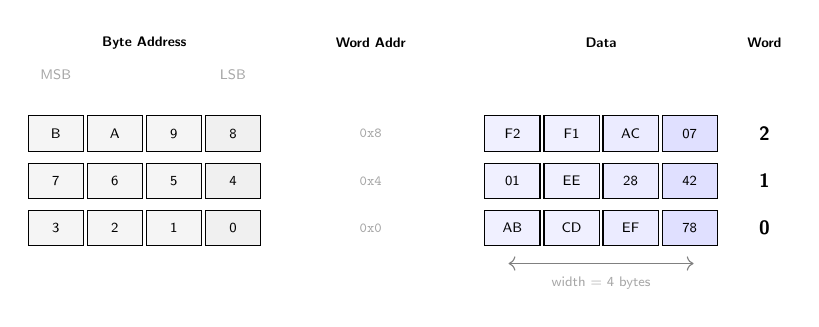
\begin{tikzpicture}[
      cell/.style={draw, minimum width=0.7cm, minimum height=0.45cm,
                   font=\sffamily\tiny, inner sep=0pt},
      hdr/.style={font=\sffamily\tiny\bfseries},
      addr/.style={font=\sffamily\tiny, text=gray!70},
      lbl/.style={font=\sffamily\scriptsize\bfseries}]

    \def\cw{0.75}  % column width
    \def\rh{0.6}   % row height

    % ===== (a) Byte addresses =====
    \node[hdr] at (1.5*\cw, 3*\rh+0.55) {Byte Address};

    \foreach \row/\bthree/\btwo/\bone/\bzero in {
        2/B/A/9/8,
        1/7/6/5/4,
        0/3/2/1/0} {
        \node[cell, fill=gray!8]  at (0*\cw, \row*\rh) {\bthree};
        \node[cell, fill=gray!8]  at (1*\cw, \row*\rh) {\btwo};
        \node[cell, fill=gray!8]  at (2*\cw, \row*\rh) {\bone};
        \node[cell, fill=gray!12] at (3*\cw, \row*\rh) {\bzero};
    }
    \node[addr] at (0*\cw, 3*\rh+0.15) {MSB};
    \node[addr] at (3*\cw, 3*\rh+0.15) {LSB};

    % ===== Word Address column =====
    \def\mx{4.0}
    \node[hdr] at (\mx, 3*\rh+0.55) {Word Addr};
    \foreach \row/\wa in {2/0x8, 1/0x4, 0/0x0} {
        \node[addr] at (\mx, \row*\rh) {\texttt{\wa}};
    }

    % ===== (b) Data =====
    \def\dx{5.8}
    \node[hdr] at (\dx+1.5*\cw, 3*\rh+0.55) {Data};

    \foreach \row/\dthree/\dtwo/\done/\dzero in {
        2/F2/F1/AC/07,
        1/01/EE/28/42,
        0/AB/CD/EF/78} {
        \node[cell, fill=blue!6]  at (\dx+0*\cw, \row*\rh) {\dthree};
        \node[cell, fill=blue!6]  at (\dx+1*\cw, \row*\rh) {\dtwo};
        \node[cell, fill=blue!8]  at (\dx+2*\cw, \row*\rh) {\done};
        \node[cell, fill=blue!12] at (\dx+3*\cw, \row*\rh) {\dzero};
    }

    % ===== Word Number column =====
    \def\wx{9.0}
    \node[hdr] at (\wx, 3*\rh+0.55) {Word};
    \foreach \row/\wn in {2/2, 1/1, 0/0} {
        \node[lbl] at (\wx, \row*\rh) {\wn};
    }

    % ===== Width annotation =====
    \draw[<->, gray] (\dx-0.05, -0.45) -- (\dx+3*\cw+0.05, -0.45);
    \node[addr] at (\dx+1.5*\cw, -0.7) {width = 4 bytes};

    \end{tikzpicture}
    \caption{Byte-addressable memory (little-endian), after Harris Figure~6.1. Left: byte addresses within each word. Right: example data values. The word address equals the byte address of the LSB (lowest address). E.g. Word \texttt{0xF2F1AC07} is stored at address \texttt{0x4}. \texttt{lw} reads all 4 bytes; \texttt{lh} reads 2 bytes; \texttt{lb} reads one byte.}
    \label{fig:mem-layout}
\end{figure}

\textbf{Load} instructions read from memory into a register: \texttt{lw rd, offset(rs1)} computes address $= \texttt{rs1} + \text{sign-extend}(\text{offset})$ and writes the 32-bit word at that address into \texttt{rd}. Sub-word loads \texttt{lh}/\texttt{lb} sign-extend; \texttt{lhu}/\texttt{lbu} zero-extend. \textbf{Store} instructions write a register to memory: \texttt{sw rs2, offset(rs1)} writes \texttt{rs2} to memory at $\texttt{rs1} + \text{offset}$.

RISC-V uses four addressing modes:

\begin{center}\small
\begin{tabular}{@{}l l l@{}}
    \toprule
    Mode & Used by & Address computation \\
    \midrule
    Register & R-type ALU & Operand is a register value \\
    Immediate & I-type ALU & Operand is a sign-extended 12-bit constant \\
    Base & Loads / stores & $\texttt{rs1} + \text{imm}_{12}$ (base + offset) \\
    PC-relative & Branches, \texttt{jal}, \texttt{auipc} & $\texttt{PC} + \text{imm}$ \\
    \bottomrule
\end{tabular}
\end{center}

The base addressing mode is what drives all memory access: the ALU computes \texttt{reg\_op1 + decoded\_imm} to produce the memory address. For memory-mapped I/O (Section~\ref{sec:mmio}), the same \texttt{lw}/\texttt{sw} instructions access peripheral registers --- the address decoder routes the transaction to the correct device.

\subsection{Programming Model}

\subsubsection{Program flow and the PC}

Instructions are stored in memory as 32-bit words (4 bytes), so consecutive instruction addresses increase by four. The \textbf{program counter (PC)} holds the address of the current instruction. After each instruction completes, the PC increments by 4 to fetch the next:

\begin{center}\small
\begin{tabular}{@{}l l@{}}
    \toprule
    Address & Instruction \\
    \midrule
    \texttt{0x538} & \texttt{addi s1, s2, s3} \\
    \texttt{0x53C} & \texttt{lw~~t2, 8(s1)} \\
    \texttt{0x540} & \texttt{sw~~s3, 3(t6)} \\
    \bottomrule
\end{tabular}
\end{center}

When the processor executes the \texttt{addi} at \texttt{0x538}, PC\,=\,\texttt{0x538}. After completion, PC increments to \texttt{0x53C} and the processor fetches \texttt{lw}. This sequential flow continues unless a branch or jump redirects the PC.

\subsubsection{Logical, shift, and multiply instructions}

Beyond arithmetic (\texttt{add}/\texttt{sub}), RV32I provides bitwise logical operations and shifts, all available in both register--register (R-type) and register--immediate (I-type) forms:

\begin{center}\small
\begin{tabular}{@{}l l l@{}}
    \toprule
    Operation & R-type & I-type \\
    \midrule
    AND / OR / XOR & \texttt{and rd, rs1, rs2} & \texttt{andi rd, rs1, imm} \\
    Shift left logical & \texttt{sll rd, rs1, rs2} & \texttt{slli rd, rs1, shamt} \\
    Shift right logical & \texttt{srl rd, rs1, rs2} & \texttt{srli rd, rs1, shamt} \\
    Shift right arithmetic & \texttt{sra rd, rs1, rs2} & \texttt{srai rd, rs1, shamt} \\
    \bottomrule
\end{tabular}
\end{center}

Shifts are particularly important for array indexing: \texttt{slli rd, rs1, 2} multiplies by 4 to convert a word index to a byte offset. The M~extension adds \texttt{mul}/\texttt{div}/\texttt{rem} (Section~\ref{sec:pcpi}), but the base ISA handles multiplication by powers of~2 via shifts.

\subsubsection{Branching and conditional statements}

RV32I provides six conditional branch instructions. All are B-type (two register sources, a 13-bit PC-relative offset):

\begin{center}\small
\begin{tabular}{@{}l l@{}}
    \toprule
    Instruction & Branches if \\
    \midrule
    \texttt{beq rs1, rs2, label} & rs1 $=$ rs2 \\
    \texttt{bne rs1, rs2, label} & rs1 $\neq$ rs2 \\
    \texttt{blt / bltu} & rs1 $<$ rs2 (signed / unsigned) \\
    \texttt{bge / bgeu} & rs1 $\geq$ rs2 (signed / unsigned) \\
    \bottomrule
\end{tabular}
\end{center}

The key assembly pattern: test the \emph{opposite} condition to \emph{skip} the block. An \texttt{if~(a==b)} in C becomes \texttt{bne a, b, skip} --- if not equal, skip the if-body. For \texttt{if/else}, the if-body ends with a \texttt{j} (unconditional jump) past the else-body:

\begin{verbatim}
    # if (s0 == s1) { s2 = s3 + s4; } else { s0 = s1 - s4; }
    bne  s0, s1, else     # skip to else if s0 != s1
    add  s2, s3, s4       # if-body
    j    done
else:
    sub  s0, s1, s4       # else-body
done:
\end{verbatim}

\texttt{switch/case} compiles to a chain of compare-and-branch pairs (load constant into a temporary, \texttt{bne} to the next case), equivalent to nested \texttt{if/else}.

\subsubsection{Loops}

All loop forms use branches. A \textbf{while} loop tests the (opposite) condition at the top and jumps back from the bottom:

\begin{verbatim}
    # while (s0 != 128) { s0 = s0 * 2; s1++; }
    addi t0, zero, 128
while: beq  s0, t0, done   # exit if s0 == 128
    slli s0, s0, 1          # s0 *= 2
    addi s1, s1, 1
    j    while
done:
\end{verbatim}

A \textbf{do/while} is identical but places the branch at the bottom (test the \emph{same} condition to continue, no initial jump). A \textbf{for} loop is syntactic sugar over while: initialisation before the loop, increment at the bottom, same opposite-condition test at the top.

\subsubsection{Arrays}

An array stores elements (bytes) at sequential addresses. For 32-bit integers, element $i$ is at address $\text{base} + 4i$. The standard access pattern multiplies the index by 4 (shift left by 2), adds the base, and uses \texttt{lw}/\texttt{sw}: \footnote{The syntax \texttt{offset(base)} denotes the memory address \texttt{base + offset}, where \texttt{base} is a register and \texttt{offset} is a 12-bit signed immediate. For example, \texttt{lw t1, 0(t0)} loads from address \texttt{t0 + 0}, and \texttt{sw s3, 8(sp)} stores to address \texttt{sp + 8}.}

\begin{verbatim}
    # scores[i] += 10,  s0 = base address of scores,  s1 = index i
    slli t0, s1, 2        # t0 = i << 2 = i * 4  (byte offset for word-sized elements)
    add  t0, t0, s0       # t0 = base + 4i = &scores[i]  (address of element i)
    lw   t1, 0(t0)        # t1 = MEM[base + 4i] = scores[i]  (load element)
    addi t1, t1, 10       # t1 = scores[i] + 10
    sw   t1, 0(t0)        # MEM[base + 4i] = t1  (store back to scores[i])
\end{verbatim}

\subsubsection{Function calls and the stack}

High-level languages use \textbf{functions} (also called procedures or subroutines) to reuse common code and make programs more modular and readable. Functions may have inputs, called \emph{arguments}, and an output, called the \emph{return value}. A well-behaved function should calculate its return value and cause no other unintended side effects. When one function calls another, the calling function (the \textbf{caller}) and the called function (the \textbf{callee}) must agree on several things: where to put the arguments, where to find the return value, and where the callee should return to when it finishes. In RISC-V, the calling convention specifies:

\begin{itemize}
    \item The caller places up to 8 arguments in \texttt{a0}--\texttt{a7} before making the call; additional arguments go on the stack.
    \item The caller stores the return address in \texttt{ra} at the same time it jumps to the callee, using \texttt{jal}.
    \item The callee places the return value in \texttt{a0} (and \texttt{a1} for 64-bit results) before returning.
    \item The callee must not overwrite any state the caller depends on. Specifically, it must leave the \emph{saved registers} (\texttt{s0}--\texttt{s11}), the return address (\texttt{ra}), the stack pointer (\texttt{sp}), and all memory above \texttt{sp} unmodified.
\end{itemize}

\paragraph{Call and return.} Two instructions handle function calls:

\begin{itemize}
    \item \textbf{\texttt{jal rd, target}} (\emph{jump and link}): jumps to the PC-relative target and simultaneously stores the return address (\texttt{PC+4}) in \texttt{rd}. By convention \texttt{rd}\,=\,\texttt{ra} (x1), so \texttt{jal func} is shorthand for \texttt{jal ra, func}.
    \item \textbf{\texttt{jalr rd, rs1, imm}} (\emph{jump and link register}): jumps to the address \texttt{rs1+imm} and stores \texttt{PC+4} in \texttt{rd}. The pseudoinstruction \texttt{ret}\,$\equiv$\,\texttt{jalr x0, ra, 0} returns by jumping to the address saved in \texttt{ra}.
\end{itemize}

A minimal example (Harris Code Example~6.22): \texttt{main} calls \texttt{simple}, which immediately returns:

\begin{verbatim}
    0x300 main: jal simple    # ra = 0x304, jump to 0x51C
    0x304 ...                 # execution resumes here after return
    ...
    0x51C simple: jr ra       # jump to address in ra (0x304)
\end{verbatim}

\texttt{jal simple} does two things at once: it jumps to the target instruction at \texttt{0x51C} and stores the return address (\texttt{0x304}, the instruction after \texttt{jal}) in \texttt{ra}. The callee returns by executing \texttt{jr ra} (= \texttt{jalr x0, ra, 0}), which jumps back to \texttt{0x304}. The \texttt{main} function then continues executing at this address.

\paragraph{Arguments and return values.} The \texttt{simple} function above is not very useful --- it receives no input and returns no output. A more realistic function, \texttt{diffofsums}, takes four arguments and returns one result. The caller places the arguments in \texttt{a0}--\texttt{a3}; the callee puts the return value in \texttt{a0}:

\begin{verbatim}
    # y = diffofsums(f, g, h, i) = (f+g)-(h+i)
    # y = diffofsums(2, 3, 4, 5)    -- caller (main)
    addi a0, zero, 2        # argument 0 = 2
    addi a1, zero, 3        # argument 1 = 3
    addi a2, zero, 4        # argument 2 = 4
    addi a3, zero, 5        # argument 3 = 5
    jal  diffofsums          # call function
    add  s7, a0, zero        # y = returned value

    diffofsums:              # -- callee
    add  t0, a0, a1          # t0 = f + g
    add  t1, a2, a3          # t1 = h + i
    sub  s3, t0, t1          # result = (f+g) - (h+i)
    add  a0, s3, zero        # put return value in a0
    jr   ra                  # return to caller
\end{verbatim}

But this version of \texttt{diffofsums} has a problem: it modifies \texttt{t0}, \texttt{t1}, and \texttt{s3}. If \texttt{main} was using any of those registers before the call, their contents would be silently corrupted. To solve this, a function must save register values on the stack before modifying them and restore them before returning.

\paragraph{The stack.} The stack is scratch memory for saving registers and storing local variables. It is a last-in-first-out (LIFO) structure: the last word pushed is the first one popped. RISC-V uses a \textbf{full descending stack}: the stack pointer \texttt{sp} (register \texttt{x2}) starts at a high address and is decremented to grow (allocate) and incremented to shrink (deallocate). The stack space a function allocates for itself is its \textbf{stack frame}.

A function that needs to save registers follows a five-step pattern:

\begin{enumerate}
    \item Decrement \texttt{sp} to make room on the stack
    \item Store (\texttt{sw}) the register values into the allocated space
    \item Execute the function body, freely using those registers
    \item Load (\texttt{lw}) the original values back from the stack
    \item Increment \texttt{sp} to deallocate the space
\end{enumerate}

Hence the stack is a temporary location to preserve the contents of registers so operations are free to read and write to registers, and then load back values when done. Code Example~6.24 shows the improved \texttt{diffofsums} that saves and restores all three registers it modifies:

\begin{verbatim}
    diffofsums:
    addi sp, sp, -12          # 1. allocate 3 words of space on stack
    sw   s3, 8(sp)            # 2. save s3, to sp+8:sp+12
    sw   t0, 4(sp)            #    save t0, to sp+4:sp+8
    sw   t1, 0(sp)            #    save t1, to sp:sp+4
    add  t0, a0, a1           # 3. now can use registers freely. t0 = f + g
    add  t1, a2, a3           #    t1 = h + i
    sub  s3, t0, t1           #    result = (f+g) - (h+i)
    add  a0, s3, zero         #    return value in a0
    lw   s3, 8(sp)            # 4. restore s3
    lw   t0, 4(sp)            #    restore t0
    lw   t1, 0(sp)            #    restore t1
    addi sp, sp, 12           # 5. deallocate
    jr   ra                   #    return
\end{verbatim}

Figure~\ref{fig:stack-frame} shows the stack before, during, and after this call. The key invariant: \texttt{sp} and all memory above it are identical before and after execution.

\begin{figure}[htbp]
    \centering
    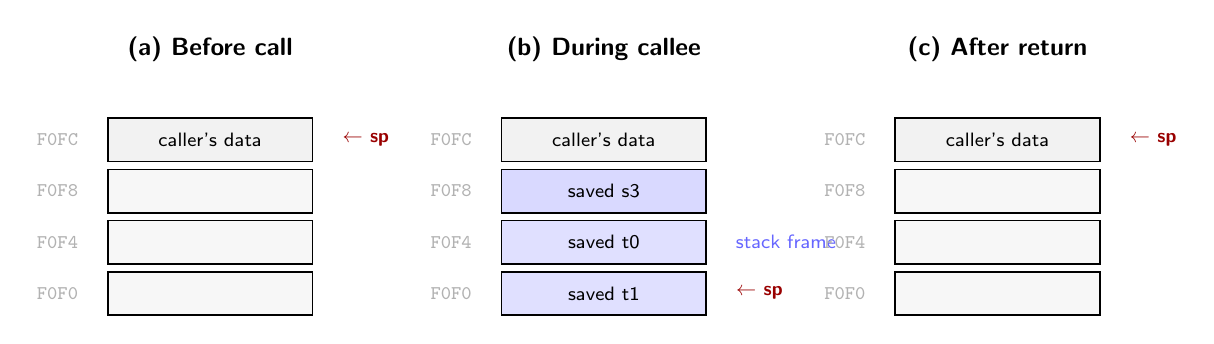
\begin{tikzpicture}[>=Stealth, semithick,
      cell/.style={draw, minimum width=2.6cm, minimum height=0.55cm,
                   font=\sffamily\scriptsize, align=center},
      addr/.style={font=\ttfamily\scriptsize, text=gray!60, anchor=east},
      sptr/.style={font=\sffamily\scriptsize\bfseries, text=red!60!black, anchor=west},
      ttl/.style={font=\sffamily\small\bfseries}]

    \def\cw{5.0}  % column spacing
    \def\rh{0.65} % row height

    % === (a) Before call ===
    \node[ttl] at (0, 3*\rh+0.5) {(a) Before call};
    \node[cell, fill=gray!10] at (0, 2*\rh) {caller's data};
    \node[cell, fill=gray!6]  at (0, 1*\rh) {};
    \node[cell, fill=gray!6]  at (0, 0) {};
    \node[cell, fill=gray!6]  at (0, -1*\rh) {};
    \node[addr] at (-1.55, 2*\rh)  {F0FC};
    \node[addr] at (-1.55, 1*\rh)  {F0F8};
    \node[addr] at (-1.55, 0)      {F0F4};
    \node[addr] at (-1.55, -1*\rh) {F0F0};
    \node[sptr] at (1.55, 2*\rh)   {$\leftarrow$ sp};

    % === (b) During callee ===
    \node[ttl] at (\cw, 3*\rh+0.5) {(b) During callee};
    \node[cell, fill=gray!10] at (\cw, 2*\rh) {caller's data};
    \node[cell, fill=blue!15] at (\cw, 1*\rh) {saved s3};
    \node[cell, fill=blue!12] at (\cw, 0)     {saved t0};
    \node[cell, fill=blue!12] at (\cw, -1*\rh) {saved t1};
    \node[addr] at (\cw-1.55, 2*\rh)  {F0FC};
    \node[addr] at (\cw-1.55, 1*\rh)  {F0F8};
    \node[addr] at (\cw-1.55, 0)      {F0F4};
    \node[addr] at (\cw-1.55, -1*\rh) {F0F0};
    \node[sptr] at (\cw+1.55, -1*\rh) {$\leftarrow$ sp};
    \node[font=\sffamily\scriptsize, text=blue!60, anchor=west] at (\cw+1.55, 0) {stack frame};

    % === (c) After return ===
    \node[ttl] at (2*\cw, 3*\rh+0.5) {(c) After return};
    \node[cell, fill=gray!10] at (2*\cw, 2*\rh) {caller's data};
    \node[cell, fill=gray!6]  at (2*\cw, 1*\rh) {};
    \node[cell, fill=gray!6]  at (2*\cw, 0)     {};
    \node[cell, fill=gray!6]  at (2*\cw, -1*\rh) {};
    \node[addr] at (2*\cw-1.55, 2*\rh)  {F0FC};
    \node[addr] at (2*\cw-1.55, 1*\rh)  {F0F8};
    \node[addr] at (2*\cw-1.55, 0)      {F0F4};
    \node[addr] at (2*\cw-1.55, -1*\rh) {F0F0};
    \node[sptr] at (2*\cw+1.55, 2*\rh)  {$\leftarrow$ sp};

    \end{tikzpicture}
    \caption{Stack before, during, and after a function call (after Harris Figure~6.8). The callee decrements \texttt{sp} by 12 to allocate a 3-word frame, saves \texttt{s3}, \texttt{t0}, and \texttt{t1}, executes, restores them, and increments \texttt{sp}. The stack is identical in (a) and (c) --- no side effects beyond \texttt{a0}.}
    \label{fig:stack-frame}
\end{figure}

\paragraph{Preserved vs.\ nonpreserved registers.} However, saving all three registers is wasteful. If the caller was not using \texttt{t0} and \texttt{t1}, the effort to save and restore them is wasted. To avoid this waste, RISC-V divides registers into \textbf{preserved} (\texttt{s0}--\texttt{s11}, \texttt{ra}, \texttt{sp} --- callee must save value to stack before modifying the register) and \textbf{nonpreserved} (\texttt{t0}--\texttt{t6}, \texttt{a0}--\texttt{a7} --- callee may freely modify register contents). Since \texttt{t0} and \texttt{t1} are nonpreserved, only \texttt{s3} actually needs saving. A \textbf{leaf function} (one that calls no others) can avoid the stack entirely by using only nonpreserved registers. A \textbf{nonleaf function} (one that calls others) must always save \texttt{ra}, since \texttt{jal} overwrites it. Recursive functions are nonleaf functions that call themselves; each invocation creates a new stack frame, so the stack grows by one frame per recursion level.

\subsubsection{Pseudoinstructions}

RISC-V keeps the hardware instruction set small; the assembler provides pseudoinstructions that expand into one or two real instructions:

\begin{center}\small
\begin{tabular}{@{}l l l@{}}
    \toprule
    Pseudo & Expands to & Effect \\
    \midrule
    \texttt{mv rd, rs} & \texttt{addi rd, rs, 0} & Copy register \\
    \texttt{li rd, imm} & \texttt{lui + addi} (or just \texttt{addi}) & Load constant \\
    \texttt{j label} & \texttt{jal x0, label} & Unconditional jump (no link) \\
    \texttt{ret} & \texttt{jalr x0, ra, 0} & Return from function \\
    \texttt{call label} & \texttt{auipc ra, ... + jalr ra, ra, ...} & Far function call \\
    \texttt{nop} & \texttt{addi x0, x0, 0} & No operation \\
    \texttt{not rd, rs} & \texttt{xori rd, rs, -1} & Bitwise NOT \\
    \bottomrule
\end{tabular}
\end{center}

\subsection{Machine Language}
  
\subsubsection{Instruction formats}

Every RV32I instruction is exactly 32 bits. The ISA defines six formats, shown in Figure~\ref{fig:rv32-formats}.

\begin{itemize}
    \item \textbf{Opcode} (\texttt{instr[6:0]}) is in the same position in every format. This lets the decoder determine the format with a single 7-bit lookup before parsing the rest of the word.
    \item \textbf{rd} (destination register, \texttt{[11:7]}), \textbf{rs1}/\textbf{rs2} (source registers, \texttt{[19:15]} and \texttt{[24:20]}) are always at fixed positions whenever they exist. Each register address is 5 bits exactly. The register file can begin reading before the full decode is complete.
    \item \textbf{funct3} (\texttt{[14:12]}) distinguishes operations within the same opcode class (e.g.\ \texttt{add} vs \texttt{and} vs \texttt{slt} all share the R-type opcode). \textbf{funct7} (\texttt{[31:25]}) provides further disambiguation in R-type: bit~5 separates \texttt{add} from \texttt{sub} and \texttt{srl} from \texttt{sra}.
    \item \textbf{The sign bit} of every immediate is always \texttt{instr[31]}.
\end{itemize}

\begin{figure}[htbp]
    \centering
    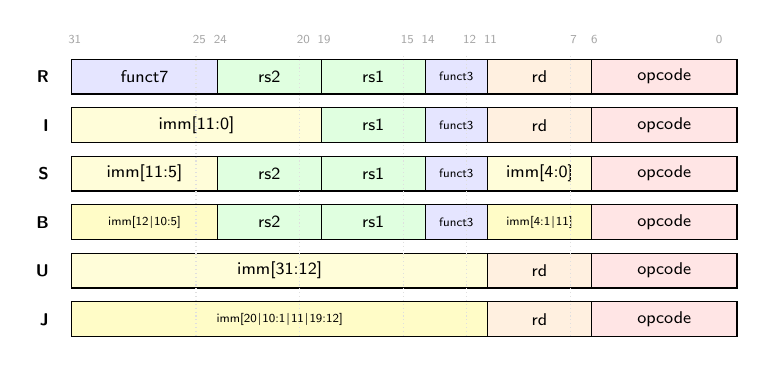
\begin{tikzpicture}[
      scale=0.88, every node/.style={transform shape},
      fld/.style={draw, minimum height=0.5cm, inner sep=0pt,
                  font=\sffamily\scriptsize, text centered},
      lbl/.style={font=\sffamily\scriptsize\bfseries, anchor=east},
      bit/.style={font=\sffamily\tiny\color{gray!70}, anchor=south}]

    % Scale: 1 bit = 0.3 cm.  Bit 31 is at x=0, bit 0 is at x=9.3
    \def\bp{0.3}        % cm per bit
    \def\rs{0.7}        % row separation

    % Bit-position ruler (top)
    \foreach \b in {31,25,24,20,19,15,14,12,11,7,6,0} {
        \pgfmathsetmacro{\xpos}{(31-\b)*\bp}
        \node[bit] at (\xpos+0.05, 0.35) {\b};
    }

    % Helper: draw a field from bit hi down to bit lo at row y
    % #1=hi, #2=lo, #3=y, #4=fill, #5=label
    \newcommand{\field}[5]{
        \pgfmathsetmacro{\xstart}{(31-#1)*\bp}
        \pgfmathsetmacro{\ww}{(#1-#2+1)*\bp}
        \node[fld, fill=#4, minimum width=\ww cm,
              anchor=west] at (\xstart, #3) {#5};
    }

    % === R-type (row 0) ===
    \node[lbl] at (-0.2, 0) {R};
    \field{31}{25}{0}{blue!10}{funct7}
    \field{24}{20}{0}{green!12}{rs2}
    \field{19}{15}{0}{green!12}{rs1}
    \field{14}{12}{0}{blue!10}{\tiny funct3}
    \field{11}{7}{0}{orange!12}{rd}
    \field{6}{0}{0}{red!10}{opcode}

    % === I-type ===
    \def\r{-\rs}
    \node[lbl] at (-0.2, \r) {I};
    \field{31}{20}{\r}{yellow!15}{imm[11:0]}
    \field{19}{15}{\r}{green!12}{rs1}
    \field{14}{12}{\r}{blue!10}{\tiny funct3}
    \field{11}{7}{\r}{orange!12}{rd}
    \field{6}{0}{\r}{red!10}{opcode}

    % === S-type ===
    \def\r{-2*\rs}
    \node[lbl] at (-0.2, \r) {S};
    \field{31}{25}{\r}{yellow!15}{imm[11:5]}
    \field{24}{20}{\r}{green!12}{rs2}
    \field{19}{15}{\r}{green!12}{rs1}
    \field{14}{12}{\r}{blue!10}{\tiny funct3}
    \field{11}{7}{\r}{yellow!15}{imm[4:0]}
    \field{6}{0}{\r}{red!10}{opcode}

    % === B-type ===
    \def\r{-3*\rs}
    \node[lbl] at (-0.2, \r) {B};
    \field{31}{25}{\r}{yellow!22}{\tiny imm[12\textbar10:5]}
    \field{24}{20}{\r}{green!12}{rs2}
    \field{19}{15}{\r}{green!12}{rs1}
    \field{14}{12}{\r}{blue!10}{\tiny funct3}
    \field{11}{7}{\r}{yellow!22}{\tiny imm[4:1\textbar11]}
    \field{6}{0}{\r}{red!10}{opcode}

    % === U-type ===
    \def\r{-4*\rs}
    \node[lbl] at (-0.2, \r) {U};
    \field{31}{12}{\r}{yellow!15}{imm[31:12]}
    \field{11}{7}{\r}{orange!12}{rd}
    \field{6}{0}{\r}{red!10}{opcode}

    % === J-type ===
    \def\r{-5*\rs}
    \node[lbl] at (-0.2, \r) {J};
    \field{31}{12}{\r}{yellow!22}{\tiny imm[20\textbar10:1\textbar11\textbar19:12]}
    \field{11}{7}{\r}{orange!12}{rd}
    \field{6}{0}{\r}{red!10}{opcode}

    % Vertical alignment guides (dashed, light)
    \foreach \b in {25,20,15,12,7} {
        \pgfmathsetmacro{\gx}{(31-\b)*\bp}
        \draw[gray!25, densely dotted] (\gx, 0.3) -- (\gx, -5*\rs-0.25);
    }

    \end{tikzpicture}
    \caption{RV32I instruction formats. Each column corresponds to a fixed bit position: \texttt{opcode} (red) is always [6:0], \texttt{rs1} (green) always [19:15], \texttt{rs2} always [24:20], \texttt{funct3} (blue) always [14:12]. Yellow fields are immediates (sign bit always at bit~31). Dotted vertical lines highlight the alignment.}
    \label{fig:rv32-formats}
\end{figure}

Table~\ref{tab:rv32-opcodes} lists the instruction classes with their operations and opcodes.

\begin{table}[htbp]
\centering\small
\renewcommand{\arraystretch}{1.45}
\makebox[\textwidth]{%
\begin{tabular}{@{} l | l | l | l | p{7.8cm} @{}}
    \toprule
    Class & Fmt & \texttt{opcode} & Operation & Description \\
    \midrule
    R-type ALU & R & \texttt{0110011} &
        \texttt{rd = rs1 op rs2} &
        Register--register arithmetic/logic. The \texttt{funct3} field selects the operation (add, sub, and, or, xor, sll, srl/sra, slt/sltu); \texttt{funct7} bit\,5 distinguishes add/sub and srl/sra. \\[2pt]
    I-type ALU & I & \texttt{0010011} &
        \texttt{rd = rs1 op imm} &
        Register--immediate: same operations as R-type, but the second operand is a 12-bit sign-extended constant from the instruction word. Shift immediates use only bits [4:0] as the shift amount. \\[2pt]
    Loads & I & \texttt{0000011} &
        \texttt{rd = Mem[rs1+imm]} &
        Reads from memory at address \texttt{rs1 + sign\_ext(imm)}. \texttt{lw} loads a full 32-bit word; \texttt{lh}/\texttt{lb} load 16/8 bits and sign-extend to 32; \texttt{lhu}/\texttt{lbu} zero-extend instead. \\[2pt]
    Stores & S & \texttt{0100011} &
        \texttt{Mem[rs1+imm] = rs2} &
        Writes \texttt{rs2} to memory at address \texttt{rs1 + sign\_ext(imm)}. No destination register --- nothing is written to the register file. The immediate is split across two fields (\texttt{[31:25]} and \texttt{[11:7]}). \\[2pt]
    Branches & B & \texttt{1100011} &
        \texttt{if(rs1 cmp rs2) PC+=imm} &
        Conditional PC-relative branch. Compares two registers and, if true, adds a 13-bit signed offset (LSB always 0) to PC. Six comparisons via \texttt{funct3}: eq, ne, lt, ge, ltu, geu. \\[2pt]
    \texttt{jal} & J & \texttt{1101111} &
        \texttt{rd=PC+4; PC+=imm} &
        Unconditional jump with link. Saves the return address (PC+4) in \texttt{rd} and adds a 21-bit signed offset to PC. Used for function calls (\texttt{rd}=\texttt{ra}) and unconditional jumps (\texttt{rd}=\texttt{x0}). \\[2pt]
    \texttt{jalr} & I & \texttt{1100111} &
        \texttt{rd=PC+4; PC=rs1+imm} &
        Jump to a register-computed address (\texttt{rs1+imm}), saving the return address in \texttt{rd}. Used for function returns (\texttt{ret} $\equiv$ \texttt{jalr x0, ra, 0}), indirect calls, and computed jumps (switch tables). \\[2pt]
    \texttt{lui} & U & \texttt{0110111} &
        \texttt{rd = imm << 12} &
        Loads a 20-bit immediate into the upper 20 bits of \texttt{rd}, zeroing the lower 12. Paired with \texttt{addi} to build arbitrary 32-bit constants (\texttt{li} pseudoinstruction). \\[2pt]
    \texttt{auipc} & U & \texttt{0010111} &
        \texttt{rd = PC+(imm<<12)} &
        Like \texttt{lui} but adds the shifted immediate to the current PC. Enables position-independent code: paired with \texttt{jalr} for far function calls, or with \texttt{lw}/\texttt{sw} for PC-relative data access. \\
    \bottomrule
\end{tabular}}
\caption{RV32I instruction classes. The Operation column shows the register-transfer semantics; the Description column explains encoding details and typical usage.}
\label{tab:rv32-opcodes}
\end{table}

Table~\ref{tab:rv32-ops-grouped} expands each class into its individual operations, showing how \texttt{funct3} (and where applicable \texttt{funct7}) selects the specific instruction within each opcode group.

\begin{table}[htbp]
\centering\small
\renewcommand{\arraystretch}{1.3}
\makebox[\textwidth]{%
\begin{tabular}{@{} l | l | l | l | l | p{9cm} @{}}
    \toprule
    \textbf{Class} & \textbf{Fmt} & \textbf{Opcode} & \textbf{f3} & \textbf{Instr} & \textbf{Operation} \\
    \midrule
    R-type ALU & R & \texttt{0110011} & 000 & \texttt{add}/\texttt{sub} &
        \texttt{rd = rs1 + rs2} or \texttt{rs1 $-$ rs2}. Distinguished by \texttt{funct7} bit\,5 (0=add, 1=sub). The only R-type pair that uses \texttt{funct7}. \\ \cline{4-6}
    & & & 001 & \texttt{sll} &
        \texttt{rd = rs1 << rs2[4:0]}. Logical shift left; vacated bits filled with 0. \\ \cline{4-6}
    & & & 010 & \texttt{slt} &
        \texttt{rd = (rs1 $<_s$ rs2) ? 1 : 0}. Signed comparison; result is 0 or 1. \\ \cline{4-6}
    & & & 011 & \texttt{sltu} &
        \texttt{rd = (rs1 $<_u$ rs2) ? 1 : 0}. Unsigned comparison. \texttt{sltu rd, x0, rs2} sets \texttt{rd}=1 if \texttt{rs2}$\neq$0. \\ \cline{4-6}
    & & & 100 & \texttt{xor} &
        \texttt{rd = rs1 \^{} rs2}. Bitwise exclusive OR. \\ \cline{4-6}
    & & & 101 & \texttt{srl}/\texttt{sra} &
        \texttt{rd = rs1 >> rs2[4:0]}. Logical or arithmetic; distinguished by \texttt{funct7} bit\,5. \\ \cline{4-6}
    & & & 110 & \texttt{or} &
        \texttt{rd = rs1 | rs2}. Bitwise OR. \\ \cline{4-6}
    & & & 111 & \texttt{and} &
        \texttt{rd = rs1 \& rs2}. Bitwise AND. \\
    \midrule
    I-type ALU & I & \texttt{0010011} & 000 & \texttt{addi} &
        \texttt{rd = rs1 + sign\_ext(imm)}. Most common instruction; \texttt{mv}, \texttt{nop}, \texttt{li} (small) are all \texttt{addi} variants. \\ \cline{4-6}
    & & & 010 & \texttt{slti} &
        \texttt{rd = (rs1 $<_s$ imm) ? 1 : 0}. Signed compare with immediate. \\ \cline{4-6}
    & & & 011 & \texttt{sltiu} &
        \texttt{rd = (rs1 $<_u$ imm) ? 1 : 0}. Unsigned compare. \texttt{sltiu rd, rs1, 1} sets \texttt{rd}=1 if \texttt{rs1}=0. \\ \cline{4-6}
    & & & 100 & \texttt{xori} &
        \texttt{rd = rs1 \^{} sign\_ext(imm)}. \texttt{xori rd, rs1, -1} is the \texttt{not} pseudoinstruction. \\ \cline{4-6}
    & & & 110 & \texttt{ori} &
        \texttt{rd = rs1 | sign\_ext(imm)}. Bitwise OR with immediate. \\ \cline{4-6}
    & & & 111 & \texttt{andi} &
        \texttt{rd = rs1 \& sign\_ext(imm)}. Bitwise AND with immediate; useful for masking bits. \\ \cline{4-6}
    & & & 001 & \texttt{slli} &
        \texttt{rd = rs1 << shamt}. Shift left by constant; \texttt{shamt} = \texttt{imm[4:0]}, upper bits must be 0. \\ \cline{4-6}
    & & & 101 & \texttt{srli}/\texttt{srai} &
        \texttt{rd = rs1 >> shamt}. Logical or arithmetic; distinguished by \texttt{imm[10]} (0=srli, 1=srai). \\
    \midrule
    Loads & I & \texttt{0000011} & 000 & \texttt{lb} &
        Load byte: \texttt{rd = sign\_ext(Mem[rs1+imm][7:0])}. Reads 8 bits, sign-extends to 32. \\ \cline{4-6}
    & & & 001 & \texttt{lh} &
        Load halfword: \texttt{rd = sign\_ext(Mem[rs1+imm][15:0])}. Reads 16 bits, sign-extends. \\ \cline{4-6}
    & & & 010 & \texttt{lw} &
        Load word: \texttt{rd = Mem[rs1+imm]}. Reads full 32 bits. Address must be 4-byte aligned. \\ \cline{4-6}
    & & & 100 & \texttt{lbu} &
        Load byte unsigned: same as \texttt{lb} but zero-extends instead of sign-extending. \\ \cline{4-6}
    & & & 101 & \texttt{lhu} &
        Load halfword unsigned: same as \texttt{lh} but zero-extends. \\
    \midrule
    Stores & S & \texttt{0100011} & 000 & \texttt{sb} &
        Store byte: \texttt{Mem[rs1+imm][7:0] = rs2[7:0]}. Writes lowest 8 bits of \texttt{rs2}. \\ \cline{4-6}
    & & & 001 & \texttt{sh} &
        Store halfword: \texttt{Mem[rs1+imm][15:0] = rs2[15:0]}. Writes lowest 16 bits. \\ \cline{4-6}
    & & & 010 & \texttt{sw} &
        Store word: \texttt{Mem[rs1+imm] = rs2}. Writes full 32 bits. \\
    \midrule
    Branches & B & \texttt{1100011} & 000 & \texttt{beq} &
        \texttt{if (rs1 == rs2) PC += imm}. \\ \cline{4-6}
    & & & 001 & \texttt{bne} &
        \texttt{if (rs1 != rs2) PC += imm}. \\ \cline{4-6}
    & & & 100 & \texttt{blt} &
        \texttt{if (rs1 $<_s$ rs2) PC += imm}. \\ \cline{4-6}
    & & & 101 & \texttt{bge} &
        \texttt{if (rs1 $\geq_s$ rs2) PC += imm}. \\ \cline{4-6}
    & & & 110 & \texttt{bltu} &
        \texttt{if (rs1 $<_u$ rs2) PC += imm}. \\ \cline{4-6}
    & & & 111 & \texttt{bgeu} &
        \texttt{if (rs1 $\geq_u$ rs2) PC += imm}. \\
    \midrule
    Jump & J & \texttt{1101111} & --- & \texttt{jal}    & \texttt{rd = PC+4; PC += sign\_ext(imm)}. 21-bit offset, $\pm$1\,MiB range. \\
    \midrule
    Jump reg. & I & \texttt{1100111} & 000 & \texttt{jalr}   & \texttt{rd = PC+4; PC = (rs1+sign\_ext(imm)) \& \~{}1}. LSB cleared for alignment. \\
    \midrule
    Upper imm. & U & \texttt{0110111} & --- & \texttt{lui}    & \texttt{rd = imm[31:12] << 12}. Upper 20 bits loaded, lower 12 zeroed. \\
    \midrule
    PC + upper & U & \texttt{0010111} & --- & \texttt{auipc}  & \texttt{rd = PC + (imm[31:12] << 12)}. PC-relative upper immediate. \\
    \bottomrule
\end{tabular}}
\caption{RV32I individual operations grouped by opcode class, showing how \texttt{funct3} (column~2) selects the specific instruction within each group. For R-type shifts and \texttt{add}/\texttt{sub}, \texttt{funct7} bit\,5 provides further disambiguation. The notation $<_s$/$<_u$ denotes signed/unsigned comparison.}
\label{tab:rv32-ops-grouped}
\end{table}

Figure~\ref{fig:instr-datapath} shows which hardware components each instruction class uses. Every instruction reads the PC and instruction memory (fetch). The differences are in what happens next: ALU instructions use the register file and ALU but skip data memory; loads and stores use all four; branches use the ALU for comparison and conditionally update the PC; jumps write PC+4 to a register and update the PC unconditionally.

\begin{figure}[htbp]
    \centering
    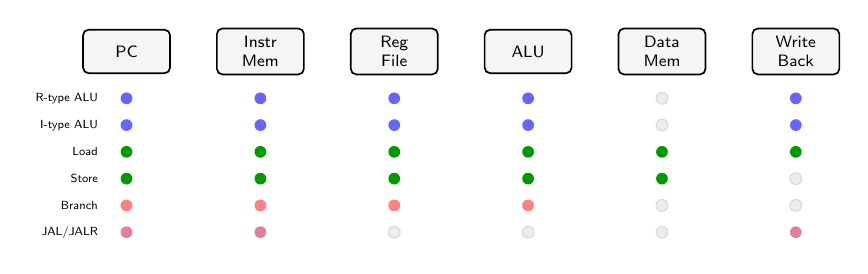
\begin{tikzpicture}[>=Stealth, semithick, scale=0.85, every node/.style={transform shape},
      blk/.style={draw, rounded corners=2pt, minimum height=0.65cm,
                  minimum width=1.3cm, font=\sffamily\scriptsize, align=center},
      used/.style={circle, fill=#1, minimum size=5pt, inner sep=0pt},
      unused/.style={circle, fill=gray!15, draw=gray!30, thin, minimum size=5pt, inner sep=0pt}]

    % Hardware blocks
    \node[blk, fill=gray!8] (pc)    at (0, 0)   {PC};
    \node[blk, fill=gray!8] (imem)  at (2, 0)   {Instr\\Mem};
    \node[blk, fill=gray!8] (rf)    at (4, 0)   {Reg\\File};
    \node[blk, fill=gray!8] (alu)   at (6, 0)   {ALU};
    \node[blk, fill=gray!8] (dmem)  at (8, 0)   {Data\\Mem};
    \node[blk, fill=gray!8] (wb)    at (10, 0)  {Write\\Back};

    % Row macro: #1=y, #2=label, #3=colour, then 6 flags (1=used, 0=unused)
    \newcommand{\instrow}[9]{%
        \node[font=\sffamily\tiny, anchor=east] at (-0.3, #1) {#2};
        \ifnum#4=1 \node[used=#3] at (0,  #1) {};\else \node[unused] at (0,  #1) {};\fi
        \ifnum#5=1 \node[used=#3] at (2,  #1) {};\else \node[unused] at (2,  #1) {};\fi
        \ifnum#6=1 \node[used=#3] at (4,  #1) {};\else \node[unused] at (4,  #1) {};\fi
        \ifnum#7=1 \node[used=#3] at (6,  #1) {};\else \node[unused] at (6,  #1) {};\fi
        \ifnum#8=1 \node[used=#3] at (8,  #1) {};\else \node[unused] at (8,  #1) {};\fi
        \ifnum#9=1 \node[used=#3] at (10, #1) {};\else \node[unused] at (10, #1) {};\fi
    }
    %                  y       label           colour            pc im rf alu dm wb
    \instrow{-0.7} {R-type ALU}{blue!60}        {1}{1}{1}{1}{0}{1}
    \instrow{-1.1} {I-type ALU}{blue!60}        {1}{1}{1}{1}{0}{1}
    \instrow{-1.5} {Load}      {green!60!black} {1}{1}{1}{1}{1}{1}
    \instrow{-1.9} {Store}     {green!60!black} {1}{1}{1}{1}{1}{0}
    \instrow{-2.3} {Branch}    {red!50}         {1}{1}{1}{1}{0}{0}
    \instrow{-2.7} {JAL/JALR}  {purple!50}      {1}{1}{0}{0}{0}{1}

    \end{tikzpicture}
    \caption{Datapath usage by instruction class. Filled dots show which stages are active; hollow dots show stages that are skipped. Every instruction uses the PC and instruction memory (fetch). ALU instructions skip data memory; stores skip writeback; branches conditionally update the PC.}
    \label{fig:instr-datapath}
\end{figure}

\subsubsection{Immediate encoding}

Immediates are shorter than 32 bits (12 bits for I-type, 13 for B-type, 21 for J-type), but the ALU operates on 32-bit values. \textbf{Sign extension} pads the immediate to 32 bits by replicating its most significant (sign) bit into all the upper positions. For example, the 12-bit value \texttt{0xFFF} ($= -1$ in two's complement) becomes \texttt{0xFFFFFFFF} (still $-1$ as a 32-bit number), while \texttt{0x001} becomes \texttt{0x00000001}. This preserves the signed value of the immediate regardless of its original width.\footnote{Since I-type immediates are only 12 bits, loading a full 32-bit constant requires two instructions: \texttt{lui} (upper 20 bits) + \texttt{addi} (lower 12); the \texttt{li} pseudoinstruction handles this.}

\paragraph{Shift immediates.} The shift instructions \texttt{slli}/\texttt{srli}/\texttt{srai} use I-type encoding but only need 5 bits for the shift amount (\texttt{shamt} = \texttt{instr[24:20]}). The upper bits (\texttt{instr[31:25]}) are repurposed as a function code: \texttt{0000000} for \texttt{slli}/\texttt{srli}, \texttt{0100000} for \texttt{srai}.

The immediate bits are deliberately arranged for regularity across formats, so most of the immediate-extraction hardware is just wiring --- only a small mux controlled by the opcode is needed for the roving bits. Because the sign bit is always at \texttt{instr[31]}, a single wire drives the sign-extension logic for all formats (see Harris Figures~6.26--6.27).

\subsubsection{The stored program}

A program in machine language is a series of 32-bit numbers stored in memory. The processor fetches them sequentially, decodes each one, executes it, and advances the PC by 4 to the next. This is the \textbf{stored program} concept: running a different program requires only writing new instructions to memory, not reconfiguring hardware. In contrast to dedicated hardware (e.g.\ a systolic array), a stored-program processor is general-purpose --- the same circuit executes any program.

The \textbf{architectural state} of a RISC-V processor is the minimal information needed to fully determine what a program will do: the \emph{register file} (32 $\times$ 32-bit registers), the \emph{program counter} (PC), and the contents of \emph{memory}. If the OS saves the architectural state at some point, it can interrupt the program, run something else, and later restore the state so the program continues as if nothing happened. The microarchitecture's job is to faithfully update the architectural state according to each instruction.

\subsection{Compiling, Assembling, Loading}

\begin{comment}
READ: Harris §6.5.1 (Memory Map, Figure 6.31)
READ: Harris §6.5.2 (Assembler Directives, Table 6.5, Code Example 6.29)
READ: Harris §6.5.3 (Compiling, Code Example 6.30 --- C to assembly via GCC)
READ: Harris §6.5.4 (Assembling --- two-pass assembly, symbol table, objdump disassembly)
READ: Harris §6.5.5 (Linking --- relocation, symbol table update, gp-relative addressing)
READ: Harris §6.5.6 (Loading --- OS loads text segment into memory, jumps to start)

CUSTOM TIKZ DIAGRAMS:
  - Toolchain flow diagram (after Harris Figure 6.30): vertical flow
    High-level code -> Compiler -> Assembly code -> Assembler -> Object file (+ Library/Object files) -> Linker -> Executable -> Loader -> Memory
    This is a key diagram showing the full translation pipeline from C to running program.

  - Memory map diagram (after Harris Figure 6.31): vertical stack showing 5 segments with addresses:
    Exception Handlers (0x00000000), Text (0x00010000, PC->), Global Data (0x10000000, gp->),
    Dynamic Data with Heap growing up and Stack growing down (sp->0xBFFFFFF0),
    OS & I/O (0xC0000000--0xFFFFFFFC).
    Note: PicoSoC uses a very different, simplified variant (Section picosoc).

CUSTOM TABLES:
  - Assembler directives table (after Harris Table 6.5): .text, .data, .bss, .section, .align N,
    .balign N, .globl sym, .string "str", .word, .byte, .space N, .equ name constant, .end

CONTENT:
  1. Toolchain overview (§6.5 intro, Figure 6.30): compiler -> assembler -> linker -> loader pipeline.
     In practice most compilers (GCC) perform all three steps.
     gcc -O1 -g prog.c -o prog (compile+assemble+link)
     gcc -O1 -S prog.c -o prog.s (compile only, see assembly)

  2. Memory map (§6.5.1, Figure 6.31):
     - Text segment: machine language instructions + literals/read-only data
     - Global data segment: global variables, accessed via gp (x3) with 12-bit signed offset
     - Dynamic data: stack (grows down from 0xBFFFFFF0, sp=x2) and heap (grows up, malloc/new)
       Stack and heap must not collide; memory allocator prevents this
     - Exception handlers: trap vectors and boot code at low addresses
     - OS/I/O: operating system and memory-mapped I/O at high addresses
     - RISC-V does NOT define a fixed memory map --- user/implementation can customise

  3. Assembler directives (§6.5.2, Table 6.5):
     - .text/.data/.bss/.section .rodata: place code/data in appropriate segments
     - .globl sym: make label visible to linker (needed for main)
     - .equ name, value: define named constant (assembler substitutes before encoding)
     - .word/.byte/.string/.space: allocate and initialise data
     - .align N / .balign N: alignment (2^N-byte or N-byte boundary)
     - Code Example 6.29: full working program using all directives, with memory layout

  4. Assembling (§6.5.4):
     - Two-pass process: pass 1 assigns addresses and builds symbol table; pass 2 generates machine code
     - Symbol table: maps label/variable names to addresses and sizes
     - objdump -S prog.o: disassemble object file (shows machine code + assembly + C if compiled with -g)
     - call pseudoinstruction expands to auipc + jalr (in case target is far)
     - Global variable addresses are placeholders until linking

  5. Linking (§6.5.5):
     - Combines object files + start-up code + libraries into single executable
     - Relocates code and data to actual addresses; updates symbol table
     - After linking: func at 0x10144, main at 0x10180, globals f/g/y in .bss at 0x11a30--0x11a38
     - Near calls optimised: call -> single jal instead of auipc+jalr
     - gp-relative stores: sw a4, -944(gp) instead of lui+sw (gp = 0x11DE0)
     - Functions may shrink after linking (func: 16->15 instr, main: 17->13 instr)

  6. Loading (§6.5.6, Figure 6.34):
     - OS reads text segment from storage (disk/flash) into text segment of memory
     - OS jumps to beginning of program to start execution
     - Figure 6.34: full memory map with prog loaded, showing every instruction word in memory
\end{comment}

\subsubsection{Toolchain overview}

Translating a high-level program into a running binary involves four stages, shown in Figure~\ref{fig:toolchain}. The \textbf{compiler} translates C into assembly language. The \textbf{assembler} converts assembly into machine code, producing an \emph{object file} containing binary instructions and a symbol table. The \textbf{linker} combines one or more object files with library code and start-up code, resolves symbol addresses, and produces a single \emph{executable}. Finally, the \textbf{loader} (typically the OS or a bootloader) copies the executable's text segment into memory and jumps to the entry point.

In practice, GCC performs all three translation steps in one command:

\begin{verbatim}
    gcc -O1 -g prog.c -o prog       # compile + assemble + link

    gcc -O1 -S prog.c -o prog.s     # compile only (view assembly)
    gcc -c prog.s -o prog.o          # assemble only (object file)

    objdump -S prog.o                # disassemble (machine + assembly + C)
\end{verbatim}

\begin{figure}[htbp]
    \centering
    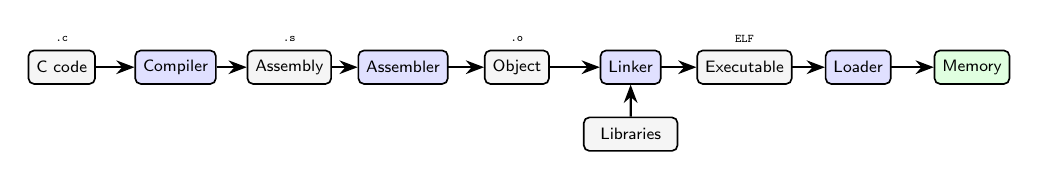
\begin{tikzpicture}[>=Stealth, semithick, scale=0.85, every node/.style={transform shape},
      file/.style={draw, rounded corners=2pt, minimum height=0.5cm,
                   font=\sffamily\scriptsize, align=center, fill=gray!8},
      tool/.style={draw, rounded corners=2pt, minimum height=0.5cm,
                   font=\sffamily\scriptsize, align=center, fill=blue!12},
      arr/.style={->, thick},
      ext/.style={font=\ttfamily\tiny}]

    \def\hs{1.7}  % horizontal spacing

    % Alternating file-tool-file-tool flow
    \node[file] (src)  at (0,      0) {C code};
    \node[tool] (comp) at (1*\hs,  0) {Compiler};
    \node[file] (asm)  at (2*\hs,  0) {Assembly};
    \node[tool] (asmr) at (3*\hs,  0) {Assembler};
    \node[file] (obj)  at (4*\hs,  0) {Object};
    \node[tool] (link) at (5*\hs,  0) {Linker};
    \node[file] (exe)  at (6*\hs,  0) {Executable};
    \node[tool] (load) at (7*\hs,  0) {Loader};
    \node[file, fill=green!12] (mem) at (8*\hs, 0) {Memory};

    % Main arrows
    \draw[arr] (src)  -- (comp);
    \draw[arr] (comp) -- (asm);
    \draw[arr] (asm)  -- (asmr);
    \draw[arr] (asmr) -- (obj);
    \draw[arr] (obj)  -- (link);
    \draw[arr] (link) -- (exe);
    \draw[arr] (exe)  -- (load);
    \draw[arr] (load) -- (mem);

    % Library files feeding into linker from below
    \node[file, minimum width=1.4cm] (lib) at (5*\hs, -1.0) {Libraries};
    \draw[arr] (lib) -- (link);

    % File extension labels above
    \node[ext] at (0,      0.42) {.c};
    \node[ext] at (2*\hs,  0.42) {.s};
    \node[ext] at (4*\hs,  0.42) {.o};
    \node[ext] at (6*\hs,  0.42) {ELF};

    \end{tikzpicture}
    \caption{Program translation pipeline (after Harris Figure~6.30). Blue boxes are tools; grey boxes are intermediate file representations. The linker combines object files with libraries to produce the final executable, which the loader places into memory.}
    \label{fig:toolchain}
\end{figure}

\subsubsection{Memory map}

With 32-bit addresses, the RISC-V address space spans $2^{32}$ bytes (4\,GB). RISC-V does \emph{not} define a fixed memory map --- implementations are free to place segments wherever suits their hardware. Figure~\ref{fig:memmap} shows the conventional layout used by Linux-class systems. The five segments serve distinct purposes:

\begin{itemize}
    \item \textbf{Text}: the machine language program (instructions), plus literals and read-only data (\texttt{.rodata}).
    \item \textbf{Global data}: global variables allocated before the program runs. Accessed via the \textbf{global pointer} \texttt{gp} (register \texttt{x3}), which points to the middle of the segment so that a single 12-bit signed offset can reach the entire range.
    \item \textbf{Dynamic data}: the \textbf{stack} (grows downward from \texttt{sp}, used for function frames and local variables) and the \textbf{heap} (grows upward, used for \texttt{malloc}/\texttt{new} allocations). If they collide, the program's data is corrupted --- the memory allocator prevents this by returning an out-of-memory error.
    \item \textbf{Exception handlers}: trap vectors and boot code at the lowest addresses.
    \item \textbf{OS and I/O}: operating system kernel and memory-mapped I/O peripherals at the highest addresses.
\end{itemize}

\begin{figure}[htbp]
    \centering
    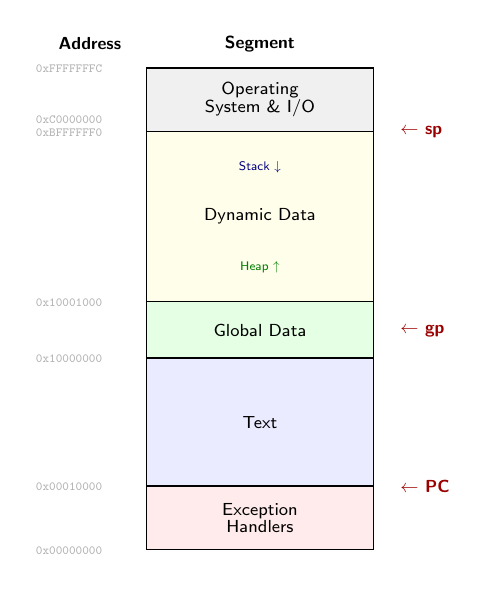
\begin{tikzpicture}[>=Stealth, semithick, scale=0.9, every node/.style={transform shape},
      seg/.style={draw, minimum width=3.2cm, inner sep=0pt,
                  font=\sffamily\scriptsize, align=center, anchor=south},
      adr/.style={font=\ttfamily\tiny, text=gray!60, anchor=east},
      ptr/.style={font=\sffamily\scriptsize\bfseries, text=red!60!black, anchor=west}]

    % Segment heights (cm)
    \def\hExc{0.9}
    \def\hText{1.8}
    \def\hGlob{0.8}
    \def\hDyn{2.4}
    \def\hOS{0.9}
    \def\sw{3.2}

    % Cumulative y positions (bottom edge of each segment)
    \pgfmathsetmacro{\yExc}{0}
    \pgfmathsetmacro{\yText}{\hExc}
    \pgfmathsetmacro{\yGlob}{\yText + \hText}
    \pgfmathsetmacro{\yDyn}{\yGlob + \hGlob}
    \pgfmathsetmacro{\yOS}{\yDyn + \hDyn}
    \pgfmathsetmacro{\yTop}{\yOS + \hOS}

    % Stacked segments (anchor=south so they tile exactly)
    \node[seg, fill=red!8,    minimum height=\hExc cm,  minimum width=\sw cm] at (0, \yExc)  {Exception\\[-1pt]Handlers};
    \node[seg, fill=blue!8,   minimum height=\hText cm, minimum width=\sw cm] at (0, \yText) {Text};
    \node[seg, fill=green!10, minimum height=\hGlob cm, minimum width=\sw cm] at (0, \yGlob) {Global Data};
    \node[seg, fill=yellow!8, minimum height=\hDyn cm,  minimum width=\sw cm] at (0, \yDyn)  {Dynamic Data};
    \node[seg, fill=gray!12,  minimum height=\hOS cm,   minimum width=\sw cm] at (0, \yOS)   {Operating\\[-1pt]System \& I/O};

    % Heap / Stack annotations inside dynamic data
    \pgfmathsetmacro{\yHeapLbl}{\yDyn + 0.5}
    \pgfmathsetmacro{\yStackLbl}{\yDyn + \hDyn - 0.5}
    \node[font=\sffamily\tiny, text=green!50!black] at (0, \yHeapLbl)  {Heap $\uparrow$};
    \node[font=\sffamily\tiny, text=blue!50!black]  at (0, \yStackLbl) {Stack $\downarrow$};

    % Column headers
    \pgfmathsetmacro{\yHdr}{\yTop + 0.35}
    \node[font=\sffamily\scriptsize\bfseries] at (-2.4, \yHdr) {Address};
    \node[font=\sffamily\scriptsize\bfseries] at (0, \yHdr) {Segment};

    % Address labels at segment boundaries (left side)
    \def\ax{-2.1}
    \node[adr] at (\ax, \yExc)  {0x00000000};
    \node[adr] at (\ax, \yText) {0x00010000};
    \node[adr] at (\ax, \yGlob) {0x10000000};
    \node[adr] at (\ax, \yDyn)  {0x10001000};
    \node[adr] at (\ax, \yOS)   {0xBFFFFFF0};
    % slight offset so 0xC0 doesn't overlap 0xBF
    \pgfmathsetmacro{\yOSlbl}{\yOS + 0.18}
    \node[adr] at (\ax, \yOSlbl) {0xC0000000};
    \node[adr] at (\ax, \yTop)  {0xFFFFFFFC};

    % Pointer labels (right side)
    \def\px{1.85}
    \pgfmathsetmacro{\yGpMid}{(\yGlob + \yDyn) / 2}
    \node[ptr] at (\px, \yText)  {$\leftarrow$ PC};
    \node[ptr] at (\px, \yGpMid) {$\leftarrow$ gp};
    \node[ptr] at (\px, \yOS)    {$\leftarrow$ sp};

    \end{tikzpicture}
    \caption{Example RISC-V memory map (after Harris Figure~6.31). Addresses increase upward. The PC initially points to the text segment; \texttt{gp} points to the middle of the global data segment; \texttt{sp} starts at the top of the stack. The heap grows upward and the stack grows downward within the dynamic data region.}
    \label{fig:memmap}
\end{figure}

\subsection{Extensions and picorv32's instruction subset}

RISC-V defines a base ISA plus optional extensions. The base ISA has 32-, 64-, and 128-bit base
instruction sets: RV32I/E, RV64I, and RV128I. The picorv32 implements \textbf{RV32IMC}:\footnote{RISC-V defines three privilege levels (M/S/U-mode) and an exception mechanism using CSRs (\texttt{mtvec}, \texttt{mcause}, \texttt{mepc}, \texttt{mscratch}). When an exception occurs, the processor saves the PC in \texttt{mepc}, records the cause in \texttt{mcause}, and jumps to the handler at \texttt{mtvec}; \texttt{mret} returns. The picorv32 runs exclusively in M-mode and handles illegal instructions and misaligned accesses via the \texttt{trap} FSM state (bit~7), which raises an IRQ. See Harris~\S6.6.2 for full details.}

\begin{center}\small
\begin{tabular}{@{}l l l l@{}}
    \toprule
    Extension & Description & Status & picorv32 \\
    \midrule
    \textbf{I} & Base 32-bit integer (Table~\ref{tab:rv32-opcodes}) & Frozen & Yes (core) \\
    \textbf{M} & Integer multiply/divide & Frozen & Yes (via PCPI) \\
    \textbf{C} & Compressed 16-bit instructions & Frozen & Yes (\texttt{COMPRESSED\_ISA}) \\
    F / D / Q & Single / double / quad floating-point & Frozen & No \\
    A & Atomic instructions & Frozen & No \\
    B & Bit manipulations & Open & No \\
    V & Vector operations & Open & No \\
    \bottomrule
\end{tabular}
\end{center}

The \textbf{M extension} adds \texttt{mul}, \texttt{mulh}, \texttt{div}, \texttt{rem} and their unsigned variants. In picorv32 these are not part of the main ALU --- they are implemented via the PCPI co-processor interface (Section~\ref{sec:pcpi}), controlled by the \texttt{ENABLE\_MUL}/\texttt{ENABLE\_DIV} parameters. The \textbf{C extension} reduces common instructions to 16 bits by using 3-bit register codes (encoding only \texttt{x8}--\texttt{x15}, the 8 most-used registers) and shorter immediates. Typically 50--60\% of instructions can be compressed, which is significant when instruction memory is limited to a few KB of EBR. The picorv32 decoder expands compressed instructions into their 32-bit equivalents before the main decode stage, so the rest of the datapath is unaware of RVC.

\subsection{Architecture comparison}

\begin{itemize}
    \item \textbf{MIPS}: very similar (same ancestry). RISC-V improvements: no branch delay slot, PC-relative jumps, fixed \texttt{rs1}/\texttt{rs2}/\texttt{rd} bit positions across all formats.
    \item \textbf{ARM}: dominates mobile/embedded. Adds CISC-like features (conditional execution, multi-register push/pop, shifted source registers) to shrink code at the cost of decoder complexity. 16 GP registers vs RISC-V's 32.
    \item \textbf{x86}: CISC, variable-length instructions (1--15 bytes), only 8 GP registers, 2-operand format, condition flags, ALU can access memory directly. Modern x86 chips internally translate CISC instructions into RISC-like micro-operations.
    \item All four are load-store except x86. RISC-V and MIPS use compare-and-branch; ARM and x86 set flags first, then branch. RISC-V is the only open-source ISA with a modular extension system (M, F, C, V, \ldots).
\end{itemize}

\newpage

\section{Microarchitectures}
\label{sec:microarch}


In this chapter, we develop three microarchitectures for RISC-V: \textbf{single-cycle}, \textbf{multicycle}, and \textbf{pipelined}. They differ in how the state elements are connected and in the amount of nonarchitectural state needed. First we discuss the architecural state:

\subsection{Architectural State and the Design Process}

Recall from Section~\ref{sec:isa} that a computer architecture is defined by its instruction set and \textbf{architectural state}. For RISC-V, the architectural state consists of the \textit{program counter} (PC) and the \textit{32 general-purpose registers} (\texttt{x0}--\texttt{x31}). Any RISC-V microarchitecture must contain all of this state. If one were to save a copy of the architectural state and the contents of memory, then turn off a computer, then turn it back on and restore everything, the computer would resume the program it was running, unaware that it had ever been powered off.

\paragraph{Datapath and control.} We divide every microarchitecture into two interacting parts:
\begin{itemize}
    \item The \textbf{datapath} operates on words of data. It contains memories, registers, ALUs, and multiplexers.
    \item The \textbf{control unit} receives the current instruction from the datapath and tells the datapath how to execute it, producing multiplexer select, register enable, and memory write signals.
\end{itemize}

A good way to design a complex system is to start with hardware containing the \textbf{state elements} --- the memories and architectural state (PC and registers). Then, add blocks of combinational logic between the state elements to compute the new state based on the current state. Since the instruction is read from one part of memory and load/store instructions access another, it is convenient to partition memory into instruction memory and data memory.

\paragraph{State elements.} Figure~\ref{fig:state-elements} shows the four state elements:

\begin{itemize}
    \item \textbf{Program counter (PC)}: a single 32-bit register. The \texttt{PCNext} input wire contains the address of next instruction. On each rising clock edge, it latches the value from this input into the register. Then after rising clock edge, its output wire contains the address of the current instruction.
    \item \textbf{Instruction memory}: read-only, single port. Takes a 32-bit address $A$ and outputs the 32-bit instruction word at that address on $RD$.
    \item \textbf{Register file}: a 32-entry $\times$ 32-bit array with \emph{two} read ports and \emph{one} write port. The two read ports ($A1 \to RD1$, $A2 \to RD2$) supply both ALU operands simultaneously --- this is why R-type instructions can read \texttt{rs1} and \texttt{rs2} in the same cycle. The write port ($A3$, $WD3$, $WE3$) writes data $WD3$ into register address $A3$ on the rising clock edge, but only when $WE3$ flag is asserted.
    \item \textbf{Data memory}: a single read/write port. If flag $WE = 0$, it reads: the word at address $A$ appears on $RD$. If $WE = 1$, it writes: data $WD$ is stored to address $A$ on the rising clock edge.
\end{itemize}

All three memories are \textit{read combinationally} --- changing the address input causes new data to appear at the output after propagation delay, with no clock edge required. The clock controls \textit{writing only}: the PC, register file, and data memory all update their stored state on the rising edge and hold it stable otherwise. This makes the processor a synchronous sequential circuit.

\paragraph{Colour convention.} Throughout this document, diagrams use a consistent RGB colour scheme:\footnote{Lighter shades distinguish sub-categories within the same family: e.g.\ darker blue for memory blocks, lighter blue for register files and buffers; darker green for the main ALU, lighter green for auxiliary compute units (e.g.\ PCPI multiplier).}

\begin{center}\small
\begin{tabular}{@{}l l l@{}}
    \toprule
    Colour & Component & Examples \\
    \midrule
    \textcolor{blue!70}{Blue} & Memory / storage & Instruction memory, data memory, register file, SPRAM, cache \\
    \textcolor{green!50!black}{Green} & Compute & ALU, DSP blocks, multipliers, PCPI modules \\
    \textcolor{red!60}{Red} & Control / decode & Decoder, FSM, error/trap states \\
    Gray & Intermediate registers / state & PC, nonarchitectural working registers \\
    \bottomrule
\end{tabular}
\end{center}

\begin{figure}[htbp]
    \centering
    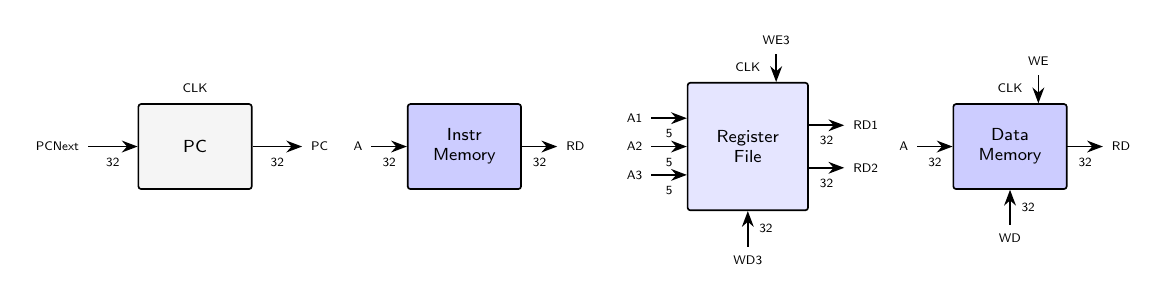
\begin{tikzpicture}[>=Stealth, semithick, scale=0.9, every node/.style={transform shape},
      blk/.style={draw, minimum height=1.2cm, minimum width=1.6cm,
                  font=\sffamily\scriptsize, align=center, rounded corners=1pt},
      port/.style={font=\sffamily\tiny},
      bw/.style={font=\sffamily\tiny, midway, below=1pt}]

    % === PC ===
    \node[blk, fill=gray!8] (pc) at (0, 0) {PC};
    \node[port] at ([yshift=6pt]pc.north) {CLK};
    \draw[<-] (pc.west) -- ++(-0.7,0) node[left, port] {PCNext} node[bw] {32};
    \draw[->] (pc.east) -- ++(0.7,0) node[right, port] {PC} node[bw] {32};

    % === Instruction Memory ===
    \node[blk, fill=blue!20] (imem) at (3.8, 0) {Instr\\Memory};
    \draw[<-] (imem.west) -- ++(-0.5,0) node[left, port] {A} node[bw] {32};
    \draw[->] (imem.east) -- ++(0.5,0) node[right, port] {RD} node[bw] {32};

    % === Register File ===
    \node[blk, fill=blue!10, minimum height=1.8cm, minimum width=1.7cm] (rf) at (7.8, 0) {Register\\File};
    \node[port] at ([yshift=6pt]rf.north) {CLK};
    \draw[<-] ([yshift=0.4cm]rf.west) -- ++(-0.5,0) node[left, port] {A1} node[bw] {5};
    \draw[<-] ([yshift=0cm]rf.west) -- ++(-0.5,0) node[left, port] {A2} node[bw] {5};
    \draw[<-] ([yshift=-0.4cm]rf.west) -- ++(-0.5,0) node[left, port] {A3} node[bw] {5};
    \draw[->] ([yshift=0.3cm]rf.east) -- ++(0.5,0) node[right, port] {RD1} node[bw] {32};
    \draw[->] ([yshift=-0.3cm]rf.east) -- ++(0.5,0) node[right, port] {RD2} node[bw] {32};
    \draw[<-] (rf.south) -- ++(0,-0.5) node[below, port] {WD3} node[midway, right=1pt, port] {32};
    \draw[<-] ([xshift=0.4cm]rf.north) -- ++(0,0.4) node[above, port] {WE3};

    % === Data Memory ===
    \node[blk, fill=blue!20, minimum height=1.2cm] (dmem) at (11.5, 0) {Data\\Memory};
    \node[port] at ([yshift=6pt]dmem.north) {CLK};
    \draw[<-] (dmem.west) -- ++(-0.5,0) node[left, port] {A} node[bw] {32};
    \draw[->] (dmem.east) -- ++(0.5,0) node[right, port] {RD} node[bw] {32};
    \draw[<-] (dmem.south) -- ++(0,-0.5) node[below, port] {WD} node[midway, right=1pt, port] {32};
    \draw[<-] ([xshift=0.4cm]dmem.north) -- ++(0,0.4) node[above, port] {WE};

    \end{tikzpicture}
    \caption{The four state elements of a RISC-V processor (after Harris Figure~7.1). The PC holds the current instruction address. The instruction memory is read-only (combinational). The register file has two read ports (A1/RD1, A2/RD2) and one clocked write port (A3/WD3/WE3). The data memory has one read/write port, clocked on writes.}
    \label{fig:state-elements}
\end{figure}

\subsection{Performance Analysis}

\begin{comment}
FIGURES TO SCREENSHOT:
  - Harris Figure 7.12 (p.407) --- complete single-cycle processor (one diagram showing the full datapath + control)
  - Harris Figure 7.27 (p.422) --- complete multicycle processor (unified memory, nonarchitectural registers)
  - Harris Figure 7.51 (p.444) --- pipelined processor with control (5-stage, pipeline registers between stages)
\end{comment}

The execution time of a program is given by the \textbf{performance equation}:

$$
T_{\text{exec}} = N_{\text{instr}} \times \text{CPI} \times T_c
$$

\begin{itemize}
    \item $N_{\text{instr}}$ (\textbf{number of instructions}): depends on the ISA and the cleverness of the programmer/compiler. For a given program on a RISC-V processor, this is constant regardless of microarchitecture.
    \item \textbf{CPI} (\textbf{cycles per instruction}): the average number of clock cycles to execute one instruction. Its reciprocal is IPC (instructions per cycle).
    \item $T_c$ (\textbf{clock period}): determined by the \textbf{critical path} through the logic. Different microarchitectures have different $T_c$ because they put different amounts of logic between pipeline registers.
\end{itemize}

The challenge of the microarchitect is to minimise $\text{CPI} \times T_c$ while satisfying constraints on cost and power. Reducing one often increases the other: adding pipeline stages reduces $T_c$ but may increase CPI due to hazards.


\subsection{Single-cycle}

A single-cycle processor executes every instruction in one clock cycle: CPI\,=\,1. The datapath reads the instruction from memory, reads registers, performs an ALU operation, accesses data memory, and writes the result back --- all in one combinational pass. The control unit is purely combinational (a truth table from opcode to control signals).

\subsubsection{Datapath} The datapath is constructed incrementally from the state elements (Figure~\ref{fig:state-elements}), adding hardware to handle each instruction class (Harris Figures~7.3--7.11):

\begin{enumerate}
    \item \textbf{Fetch}: PC provides the address to instruction memory; the 32-bit output is the instruction word \texttt{Instr}.
    \item \textbf{Register read}: \texttt{Instr[19:15]} (rs1) addresses register file port A1 into RD1, producing \texttt{SrcA}\,=\,RD1. For R-type/branches, \texttt{Instr[24:20]} (rs2) addresses port A2 into RD2, producing \texttt{SrcB}=RD2.
    \item \textbf{Sign extension}: the Extend unit extracts the immediate field and sign-extends it to 32~bits. A 2-bit \texttt{ImmSrc} control signal selects which format (I/S/B/J) to extract.
    \item \textbf{ALU}: computes \texttt{SrcA op SrcB}. The \texttt{ALUSrc} mux selects \texttt{SrcB} from either RD2 (R-type, branches) or \texttt{ImmExt} (I-type ALU, loads, stores). The 3-bit \texttt{ALUControl} selects the operation.\footnote{The ALU only accepts 32-bit because that is the register width --- both operands are always full 32-bit values (immediates are sign-extended before reaching the ALU). For data wider than 32 bits, software decomposes the operation: e.g.\ a 64-bit add uses two instructions (add lower halves, then add-with-carry upper halves). This overhead is why 32-bit ISAs eventually transition to 64-bit (ARMv7$\to$AArch64, x86$\to$x86-64).}
    \item \textbf{Data memory}: for \texttt{lw}, \texttt{ALUResult} is the address of where to load data from, and \texttt{ReadData} returns the loaded word. For \texttt{sw}, \texttt{MemWrite} flag is asserted, where RD2 feeds \texttt{WriteData} to the address at \texttt{ALUResult}.
    \item \textbf{Writeback}: the \texttt{ResultSrc} mux selects \texttt{Result} from \texttt{ALUResult} (R-type, I-type ALU), \texttt{ReadData} (\texttt{lw}), or \texttt{PCPlus4} (\texttt{jal}). This feeds the data \texttt{Result} into the register file write port WD3 (gated by \texttt{RegWrite}), and writes into the address at A3.
    \item \textbf{PC update}: one adder computes \texttt{PCPlus4}\,=\,PC+4. Another computes \texttt{PCTarget}\,=\,PC+\texttt{ImmExt} for branches/jumps. The \texttt{PCSrc} mux (driven by \texttt{Branch}\,\texttt{\&}\,\texttt{Zero}, or \texttt{Jump}) selects \texttt{PCNext}.
\end{enumerate}

Figure~\ref{fig:single-cycle-detail} shows the complete single-cycle processor. The key design strategy: compute \emph{all} possible results in parallel (\texttt{ALUResult}, \texttt{ReadData}, \texttt{PCPlus4}, \texttt{PCTarget}), then use multiplexers (select bits driven by wires from control unit) to select the correct one. Hardware operates in parallel --- unlike software, which computes sequentially. \footnote{To support \texttt{jal}, the \texttt{ResultSrc} mux is expanded from 2:1 to 3:1 (adding \texttt{PCPlus4} as input~10), and a \texttt{Jump} signal is OR'd with (\texttt{Branch}~\texttt{\&}~\texttt{Zero}) to drive \texttt{PCSrc} (Harris Figures~7.15--7.16).}

\begin{figure}[htbp]
    \centering
    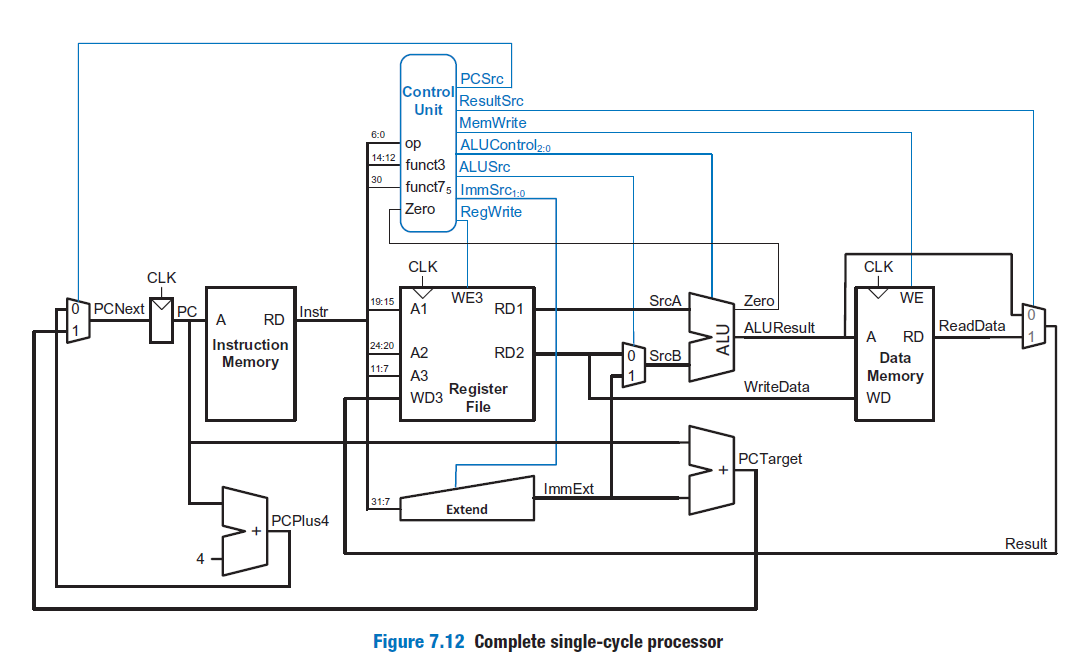
\includegraphics[width=0.95\textwidth]{figures/fig7.12.png}
    \caption{Complete single-cycle RISC-V processor (Harris Figure~7.12). The datapath flows left to right: PC $\to$ instruction memory $\to$ register file $\to$ ALU $\to$ data memory. Blue signals are control outputs. The three key multiplexers --- \texttt{ALUSrc} (selects RD2 or \texttt{ImmExt} as \texttt{SrcB}), \texttt{ResultSrc} (selects \texttt{ALUResult} or \texttt{ReadData}), and \texttt{PCSrc} (selects \texttt{PCPlus4} or \texttt{PCTarget}) --- route data differently depending on the instruction type.}
    \label{fig:single-cycle-detail}
\end{figure}

\subsubsection{Control unit} The controller decomposes into a \textbf{Main Decoder} and an \textbf{ALU Decoder} (Figure~\ref{fig:control-unit}). The Main Decoder maps \texttt{opcode[6:0]} to most control signals plus an internal 2-bit \texttt{ALUOp}. The ALU Decoder combines \texttt{ALUOp} with \texttt{funct3} (and sometimes \texttt{op$_5$}, \texttt{funct7$_5$}) to produce \texttt{ALUControl[2:0]}: \footnote{The ALU Decoder uses only 7 bits total: \texttt{ALUOp} (2 bits from the Main Decoder), all 3 bits of \texttt{funct3}, and two \emph{individual} bits --- \texttt{op$_5$} (\texttt{instr[5]}, one bit from the opcode) and \texttt{funct7$_5$} (\texttt{instr[30]}, one bit from funct7).}

\begin{figure}[htbp]
    \centering
    \begin{minipage}[t]{0.30\textwidth}
        \vspace{0pt}
        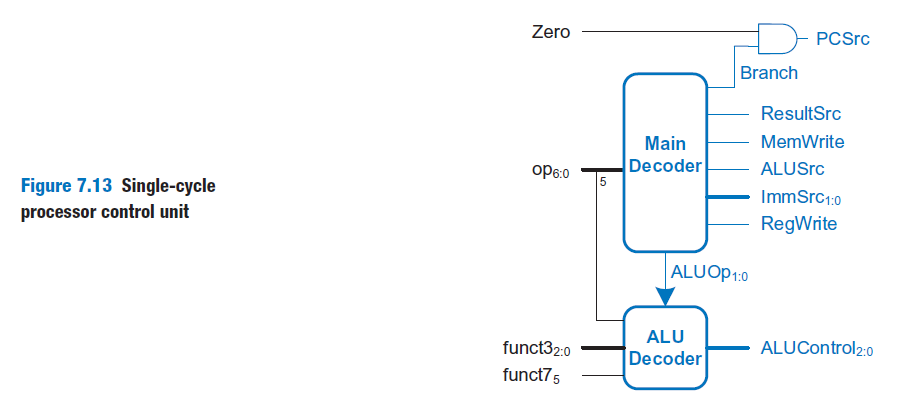
\includegraphics[width=\textwidth]{figures/fig7.13.png}
    \end{minipage}%
    \hfill
    \begin{minipage}[t]{0.68\textwidth}
        \vspace{0pt}
        \centering\footnotesize
        \renewcommand{\arraystretch}{1.05}
        \setlength{\tabcolsep}{3pt}
        \begin{tabular}{@{}l l c c c c c c c c@{}}
            \toprule
            Instr & Opcode & RegW & ImmSrc & ALUSrc & MemW & ResSrc & Br & ALUOp & Jmp \\
            \midrule
            \texttt{lw}  & \texttt{0000011} & 1 & 00 & 1 & 0 & 01 & 0 & 00 & 0 \\
            \texttt{sw}  & \texttt{0100011} & 0 & 01 & 1 & 1 & xx & 0 & 00 & 0 \\
            R-type       & \texttt{0110011} & 1 & xx & 0 & 0 & 00 & 0 & 10 & 0 \\
            \texttt{beq} & \texttt{1100011} & 0 & 10 & 0 & 0 & xx & 1 & 01 & 0 \\
            I-type ALU   & \texttt{0010011} & 1 & 00 & 1 & 0 & 00 & 0 & 10 & 0 \\
            \texttt{jal} & \texttt{1101111} & 1 & 11 & x & 0 & 10 & 0 & xx & 1 \\
            \bottomrule
        \end{tabular}

        \vspace{6pt}
        \begin{tabular}{@{}c c c c l@{}}
            \toprule
            ALUOp & funct3 & \{op$_5$, f7$_5$\} & ALUControl & Instruction \\
            \midrule
            00 & x   & x  & 000 (add) & \texttt{lw}, \texttt{sw} \\
            01 & x   & x  & 001 (sub) & \texttt{beq} \\
            10 & 000 & $\neq$11 & 000 (add) & \texttt{add}, \texttt{addi} \\
            10 & 000 & 11 & 001 (sub) & \texttt{sub} \\
            10 & 010 & x  & 101 (slt) & \texttt{slt}, \texttt{slti} \\
            10 & 110 & x  & 011 (or)  & \texttt{or}, \texttt{ori} \\
            10 & 111 & x  & 010 (and) & \texttt{and}, \texttt{andi} \\
            \bottomrule
        \end{tabular}
    \end{minipage}
    \caption{Single-cycle control unit (Harris Figure~7.13). Left: the Main Decoder maps \texttt{opcode} to control signals + \texttt{ALUOp}; the ALU Decoder refines \texttt{ALUOp} using \texttt{funct3}/\texttt{funct7$_5$}. Right top: Main Decoder truth table (\texttt{x}\,=\,don't care). Right bottom: ALU Decoder truth table --- \texttt{ALUOp}\,=\,00 always adds, 01 always subtracts, 10 inspects \texttt{funct3}/\texttt{funct7}.}
    \label{fig:control-unit}
    \label{tab:main-decoder}
    \label{tab:alu-decoder}
\end{figure}


\subsubsection{Critical path} The clock period $T_c$ is set by the slowest instruction (\texttt{lw}), whose critical path traverses: PC clk-to-Q $\to$ instruction memory $\to$ register file read $\to$ ALU $\to$ data memory $\to$ Result mux $\to$ register file setup:

$$
T_{c,\text{single}} = t_{\text{pcq}} + 2\,t_{\text{mem}} + t_{\text{RFread}} + t_{\text{ALU}} + t_{\text{mux}} + t_{\text{RFsetup}}
$$

Every instruction pays this worst-case penalty. The processor also needs separate instruction and data memories, since both are read in the same cycle.

\subsection{Multicycle}

A multicycle processor breaks each instruction into shorter steps (fetch, decode, execute, memory access, writeback), using one clock cycle per step. This has three advantages:

\begin{enumerate}
    \item $T_c$ is set by the slowest \emph{step}, not the slowest instruction --- typically a single memory access or ALU operation, roughly $\frac{1}{3}$ to $\frac{1}{5}$ of the single-cycle $T_c$. Hence $T_c$ decreases.
    \item Simple instructions finish in fewer cycles (branches: 3, R-type: 4, loads: 5), so average CPI is less than the worst case.
    \item Hardware is \textbf{reused}: a single ALU handles address calculation, arithmetic, and PC increment on different cycles; a single memory serves both instructions and data.
\end{enumerate}

The cost is a \textbf{finite state machine (FSM)} controller that sequences the control signals differently on each cycle, and \textbf{nonarchitectural registers} to hold intermediate results between steps.

\subsubsection{Datapath} Figure~\ref{fig:multicycle-detail} shows the complete multicycle processor. The key structural differences from the single-cycle design (Figure~\ref{fig:single-cycle-detail}) are:

\begin{itemize}
    \item \textbf{Unified memory}: a single memory serves both instructions and data. The \texttt{AdrSrc} multiplexer selects the address: the PC during Fetch state, or \texttt{ALUOut} (the computed data address) during MemRead/MemWrite.
    \item \textbf{Nonarchitectural registers} hold intermediate results between FSM steps:
    \begin{itemize}
        \item \texttt{Instr}: Instruction register (IR): latched on Fetch state, holds the instruction word for later steps (cycles)
        \item \texttt{OldPC}: saves the current PC address (before it is updated to PC+4), which is needed for branch/jump target computation.
        \item \texttt{A} and \texttt{WriteData}: hold the register file outputs (rs1 and rs2) read during Decode.
        \item \texttt{ALUOut}: stores the ALU result between steps (address, arithmetic result, or branch target).
        \item \texttt{Data}: holds the word read from memory during MemRead.
    \end{itemize}
    \item \textbf{Wider ALU source multiplexers}: because the ALU is reused for different purposes on different steps, the source muxes have more inputs. \texttt{ALUSrcA} selects among PC (for PC+4), \texttt{OldPC} (for branch targets), or \texttt{A} (for arithmetic/address calc). \texttt{ALUSrcB} selects among \texttt{WriteData} (R-type rs2), \texttt{ImmExt} (immediates), or the constant~4 (for PC+4).
    \item \textbf{Result multiplexer} (3 inputs): ALUOut (registered ALU results), Data (memory loads), or ALUResult (unregistered, used for PC+4 writeback during Fetch to save a cycle).
\end{itemize}

\begin{figure}[htbp]
    \centering
    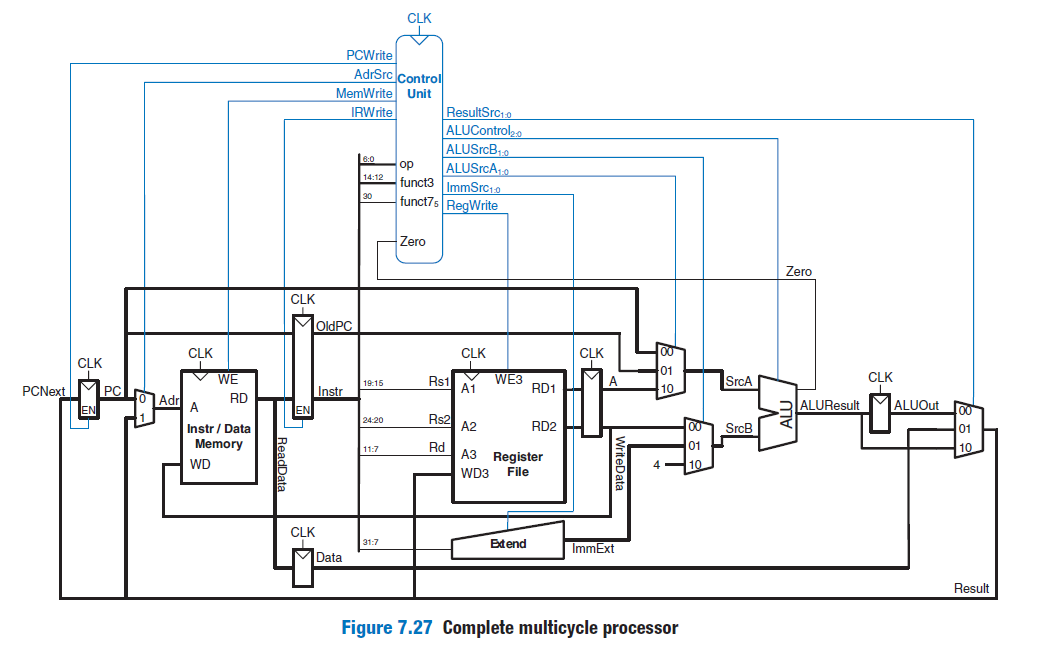
\includegraphics[width=0.7\textwidth]{figures/fig7.27.png}
    \caption{Complete multicycle RISC-V processor (Harris Figure~7.27). The datapath (black) uses a unified instruction/data memory and a single ALU, connected through nonarchitectural registers (Instr, OldPC, A, WriteData, ALUOut, Data). The control unit (blue) is an FSM that produces different control signals on each step. Compare with the single-cycle processor in Figure~\ref{fig:single-cycle-detail}: the multicycle design eliminates two adders and one memory at the cost of six nonarchitectural registers and wider multiplexers.}
    \label{fig:multicycle-detail}
\end{figure}

\subsubsection{FSM control} The controller is a Moore FSM with 11 states (Figure~\ref{fig:multicycle-fsm}). All instructions share Fetch and Decode; after Decode, the opcode determines which path to take:

\begin{center}\small
\begin{tabular}{@{}l l c@{}}
    \toprule
    Instruction & State path & Cycles \\
    \midrule
    \texttt{lw}    & Fetch $\to$ Decode $\to$ MemAdr $\to$ MemRead $\to$ MemWB & 5 \\
    \texttt{sw}    & Fetch $\to$ Decode $\to$ MemAdr $\to$ MemWrite & 4 \\
    R-type ALU     & Fetch $\to$ Decode $\to$ ExecuteR $\to$ ALUWB & 4 \\
    I-type ALU     & Fetch $\to$ Decode $\to$ ExecuteI $\to$ ALUWB & 4 \\
    \texttt{beq}   & Fetch $\to$ Decode $\to$ BEQ & 3 \\
    \texttt{jal}   & Fetch $\to$ Decode $\to$ JAL $\to$ ALUWB & 4 \\
    \bottomrule
\end{tabular}
\end{center}

Table~\ref{tab:multicycle-states} details each state: the ALU mux selects (--- when the ALU is idle), the micro-operation in register-transfer notation, and a description of what happens and why. States where the ALU is idle perform pure data routing --- moving data between nonarchitectural registers, memory, and the register file via multiplexers and write-enable signals.

\begin{table}[htbp]
\centering\scriptsize
\setlength{\tabcolsep}{4pt}
\renewcommand{\arraystretch}{1.25}
\makebox[\textwidth]{%
\begin{tabular}{@{}r l c c c l p{5.8cm}@{}}
    \toprule
    \# & State & SrcA & SrcB & Op & Micro-operation & Description \\
    \midrule
    S0 & Fetch    & PC    & 4   & add
        & \strutrow\texttt{Instr $\leftarrow$ Mem[PC]}
        & Read instruction from memory at the PC address and latch into IR. \\[4pt]
    \cline{6-7}
    & & & & & \strutrow\texttt{PC $\leftarrow$ PC+4}
        & ALU computes PC+4 and writes back to PC --- reusing the ALU that is otherwise idle this cycle. \\[4pt]
    \midrule
    S1 & Decode   & OldPC & Imm & add
        & \strutrow\texttt{A $\leftarrow$ rs1}
        & Read source registers from register file into nonarchitectural registers. \\[4pt]
    \cline{6-7}
    & & & & & \strutrow\texttt{WriteData $\leftarrow$ rs2}
        & If dual-port, rs2 read simultaneously. \\[4pt]
    \cline{6-7}
    & & & & & \strutrow\texttt{ALUOut $\leftarrow$ OldPC+ImmExt}
        & ALU speculatively computes branch target. If not a branch, this result is unused. \\[4pt]
    \midrule
    S2 & MemAdr   & A     & Imm & add
        & \strutrow\texttt{ALUOut $\leftarrow$ A + ImmExt}
        & Compute data memory address (base + offset). Shared by \texttt{lw} and \texttt{sw}. \\[4pt]
    \midrule
    S3 & MemRead  & ---   & --- & ---
        & \strutrow\texttt{Data $\leftarrow$ Mem[ALUOut]}
        & AdrSrc=1 routes ALUOut to memory address port. Data latched into Data register. \\[4pt]
    \midrule
    S4 & MemWB    & ---   & --- & ---
        & \strutrow\texttt{rd $\leftarrow$ Data}
        & ResultSrc=01 selects Data. RegWrite asserted; loaded value written to \texttt{rd}. \\[4pt]
    \midrule
    S5 & MemWrite & ---   & --- & ---
        & \strutrow\texttt{Mem[ALUOut] $\leftarrow$ rs2}
        & AdrSrc=1 routes ALUOut to memory. MemWrite asserted; WriteData written to memory. \\[4pt]
    \midrule
    S6 & ExecuteR & A     & B   & op
        & \strutrow\texttt{ALUOut $\leftarrow$ A \textit{op} B}
        & R-type ALU operation. Specific op selected by funct3/funct7 via ALU Decoder. \\[4pt]
    \midrule
    S7 & ALUWB    & ---   & --- & ---
        & \strutrow\texttt{rd $\leftarrow$ ALUOut}
        & ResultSrc=00 selects ALUOut. RegWrite asserted. Shared by R-type, I-type, and \texttt{jal}. \\[4pt]
    \midrule
    S8 & ExecuteI & A     & Imm & op
        & \strutrow\texttt{ALUOut $\leftarrow$ A \textit{op} ImmExt}
        & Same as ExecuteR but SrcB is sign-extended immediate. Handles \texttt{addi}, \texttt{andi}, \texttt{ori}, \texttt{slti}. \\[4pt]
    \midrule
    S9 & JAL      & OldPC & 4   & add
        & \strutrow\texttt{PC $\leftarrow$ ALUOut}
        & Write jump target (from Decode's speculative computation) to PC via Result mux. \\[4pt]
    \cline{6-7}
    & & & & & \strutrow\texttt{ALUOut $\leftarrow$ OldPC+4}
        & ALU computes return address OldPC+4, to be written to \texttt{rd} in next state (ALUWB). \\[4pt]
    \midrule
    S10 & BEQ     & A     & B   & sub
        & \strutrow\texttt{if Zero: PC $\leftarrow$ ALUOut}
        & ALU subtracts rs1$-$rs2. If zero (equal), Branch=1 asserts PCWrite; branch target (ALUOut from Decode) overwrites PC. Otherwise PC keeps PC+4 from Fetch. \\[4pt]
    \bottomrule
\end{tabular}}
\caption{Complete multicycle FSM state table. SrcA/SrcB/Op show ALU mux selects (--- = ALU idle). \texttt{\textbackslash midrule} separates states; \texttt{\textbackslash cline} separates micro-ops within a state.}
\label{tab:multicycle-states}
\end{table}

\begin{figure}[htbp]
    \centering
    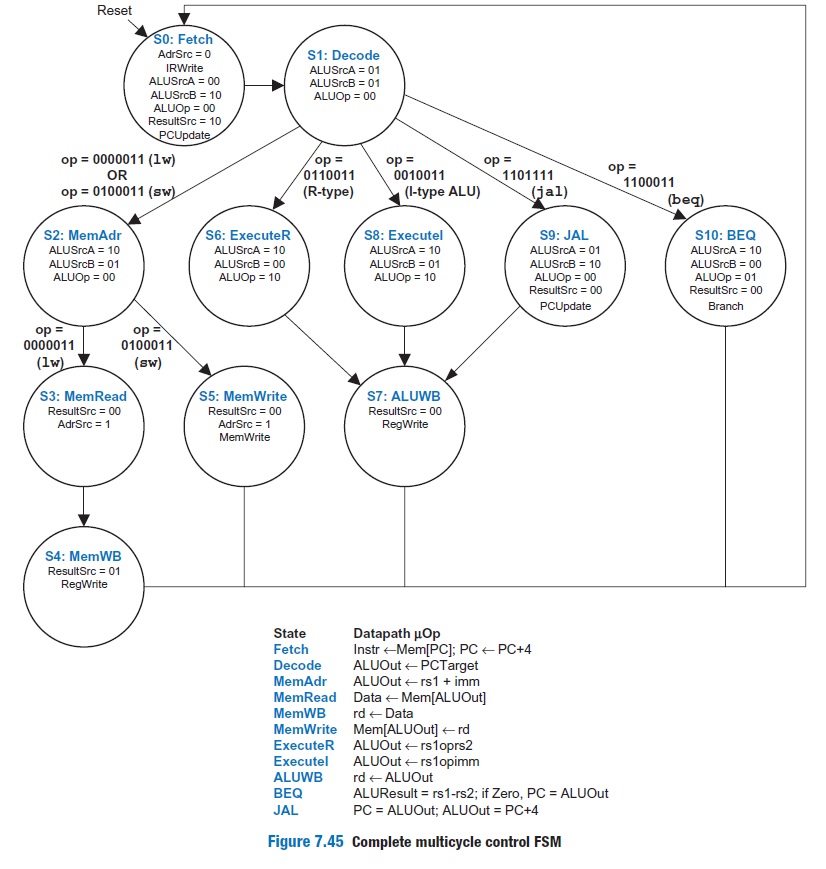
\includegraphics[width=0.6\textwidth,keepaspectratio]{figures/fig7.45.png}
    \caption{Complete multicycle control FSM with 11 states (Harris Figure~7.45). Fetch and Decode are shared by all instructions; subsequent states branch by opcode. The table summarises each state's micro-operation. Compare with picorv32's 8-state one-hot FSM (Figure~\ref{fig:picorv32-fsm}): picorv32 merges Decode into \texttt{ld\_rs1}, uses a single \texttt{exec} state for all ALU/branch/jump operations, and defers writeback to the next Fetch.}
    \label{fig:multicycle-fsm}
\end{figure}

\paragraph{Data flow example: \texttt{lw}.} Figure~\ref{fig:multicycle-dataflow} traces data through the datapath during the first three steps of \texttt{lw}, with each step colour-coded:

\begin{enumerate}
    \item \textbf{Fetch} (grey): PC drives the memory address; the instruction word flows into IR. Simultaneously, the ALU adds PC\,+\,4 and writes the result back to PC via the Result mux (ResultSrc\,=\,10).
    \item \textbf{Decode} (medium blue): \texttt{Instr[19:15]} (rs1) addresses the register file; the base address is latched into A. The Extend unit produces ImmExt from the I-type immediate field. The ALU speculatively computes OldPC\,+\,ImmExt for a potential branch target.
    \item \textbf{MemAdr} (dark blue): the ALU adds A\,+\,ImmExt (ALUSrcA\,=\,10, ALUSrcB\,=\,01, ALUOp\,=\,00) to produce the memory address, stored in ALUOut.
    \item \textbf{MemRead}: the AdrSrc mux switches to 1, routing ALUOut (the computed address) to the memory address input. The memory reads from this address and the result is latched into the Data nonarchitectural register at the end of the cycle.
    \item \textbf{MemWB}: the Result mux selects Data (ResultSrc\,=\,01), placing the loaded word on the register file's WD3 input. RegWrite is asserted, so at the next rising clock edge the value is written into the destination register rd (specified by \texttt{Instr[11:7]}).
\end{enumerate}

\begin{figure}[htbp]
    \centering
    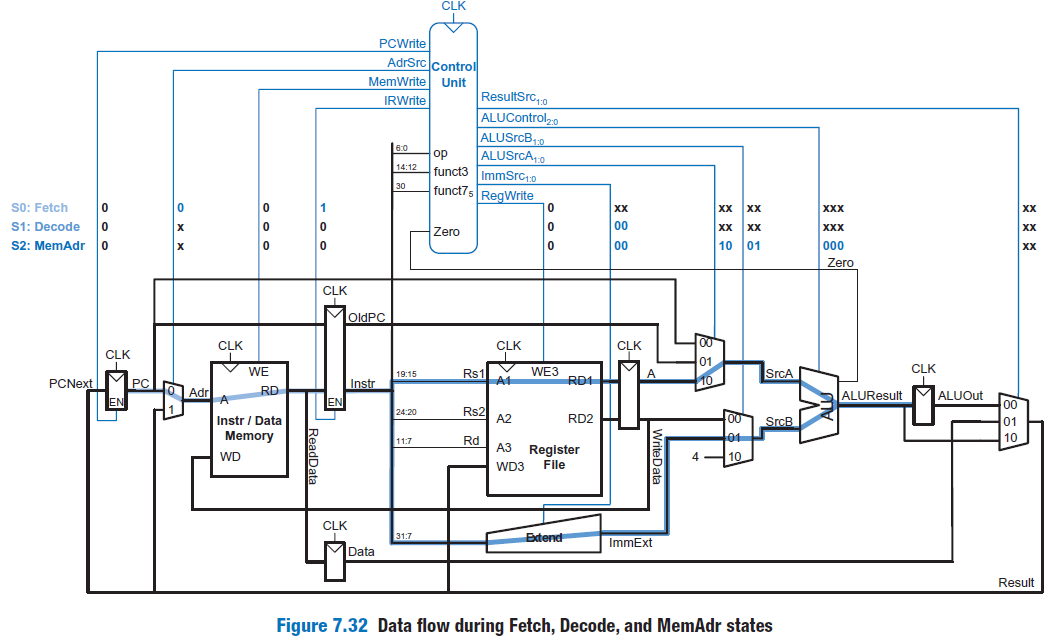
\includegraphics[width=0.7\textwidth]{figures/fig7.32.png}
    \caption{Data flow during Fetch, Decode, and MemAdr for \texttt{lw} (Harris Figure~7.32). Grey: Fetch (instruction read + PC+4). Medium blue: Decode (register read + speculative branch target). Dark blue: MemAdr (base + offset address computation). The control signal values for each state are shown in the table at top.}
    \label{fig:multicycle-dataflow}
\end{figure}

\subsubsection{Critical path} The cycle time is set by the slower of two paths (Harris Figure~7.46): (1)~the PC+4 path through the SrcA mux, ALU, and Result mux back to the PC register; or (2)~the memory read path through the Result and Adr muxes to memory into the Data register. Both paths include a decoder delay after the FSM state updates:

$$
T_{c,\text{multi}} = t_{\text{pcq}} + t_{\text{dec}} + 2\,t_{\text{mux}} + \max\!\left[t_{\text{ALU}},\; t_{\text{mem}}\right] + t_{\text{setup}}
$$

With the 7\,nm delays from Harris Table~7.7, $T_{c,\text{multi}} = 40 + 25 + 2(30) + 200 + 50 = 375$\,ps --- half the single-cycle $T_c$ of 750\,ps. But the average CPI of 4.14 (SPECINT2000 mix) more than cancels this gain: total execution time $T_{exec}$ is 155\,s versus 75\,s for single-cycle. The fundamental problem is that splitting \texttt{lw} into 5~steps does not reduce $T_c$ fivefold: the steps are unequal in length, and the 90\,ps sequencing overhead ($t_{\text{pcq}} + t_{\text{setup}}$) is paid on \emph{every} step.

The multicycle processor's advantage is hardware cost: one memory instead of two, one ALU instead of three adders, no pipeline registers, no hazard unit. This matters on the iCE40UP5K with only 5280 LUTs and 15\,KB of EBR --- which is exactly why picorv32 uses a multicycle architecture.

\subsection{Pipelined}

A pipelined processor subdivides the single-cycle datapath into five stages separated by pipeline registers. Five instructions execute simultaneously, one in each stage. Because each stage has only one-fifth of the logic, the clock frequency is approximately five times faster. Ideally the latency of each instruction is unchanged, but the throughput is five times better. Pipelining introduces some overhead (sequencing, hazards), so the speedup is less than five in practice --- but the advantage is so large that all modern high-performance processors are pipelined.

\paragraph{Pipeline stages and operation.} The five stages each involve exactly one of the slow hardware blocks (memory read, register file, or ALU):

\begin{enumerate}
    \item \textbf{Fetch (F)}: read the instruction from instruction memory at the address in PC.
    \item \textbf{Decode (D)}: read source operands from the register file and decode the instruction to produce control signals.
    \item \textbf{Execute (E)}: the ALU performs the computation (arithmetic, address calculation, or branch comparison).
    \item \textbf{Memory (M)}: read or write data memory for loads and stores.
    \item \textbf{Writeback (W)}: write the result back to the register file.
\end{enumerate}

Figure~\ref{fig:pipeline-abstract} shows six instructions flowing through the pipeline. Reading across a row shows when a particular instruction occupies each stage; reading down a column shows what all five stages are doing on a given cycle. For example, in cycle~6, the register file is writing a sum to \texttt{s3}, the data memory is idle, the ALU is computing \texttt{s11~\&~t0}, \texttt{t4} is being read from the register file, and the \texttt{or} instruction is being fetched. The instruction memory and ALU are active every cycle; the data memory is used only by loads and stores.

\begin{figure}[htbp]
    \centering
    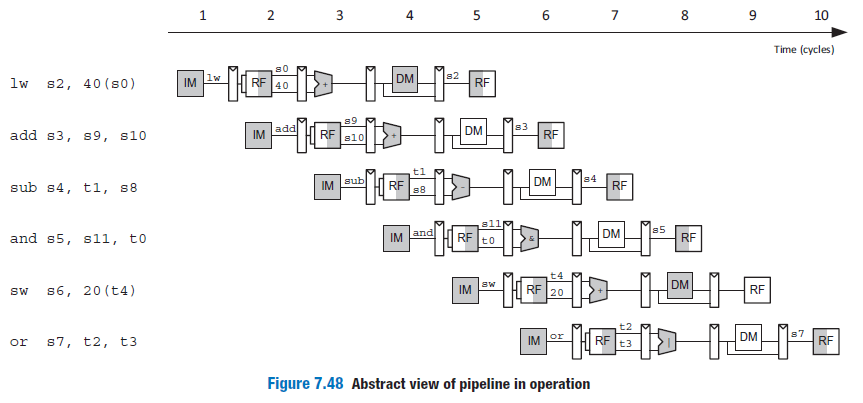
\includegraphics[width=0.95\textwidth]{figures/fig7.48.png}
    \caption{Abstract view of the pipeline in operation (Harris Figure~7.48). Each stage is represented by its major component: IM (instruction memory), RF (register file read), ALU, DM (data memory), RF (register file writeback). The register file is written in the first half of the cycle and read in the second half, so data can be written by one instruction and read by the next within a single cycle.}
    \label{fig:pipeline-abstract}
\end{figure}

\subsubsection{Datapath} The pipelined datapath is formed by inserting four pipeline registers into the single-cycle datapath (Figure~\ref{fig:single-cycle-detail}), separating it into five stages. Figure~\ref{fig:pipeline-datapath} shows the result. Signals carry a suffix (F, D, E, M, or W) indicating the stage in which they reside.

\begin{figure}[htbp]
    \centering
    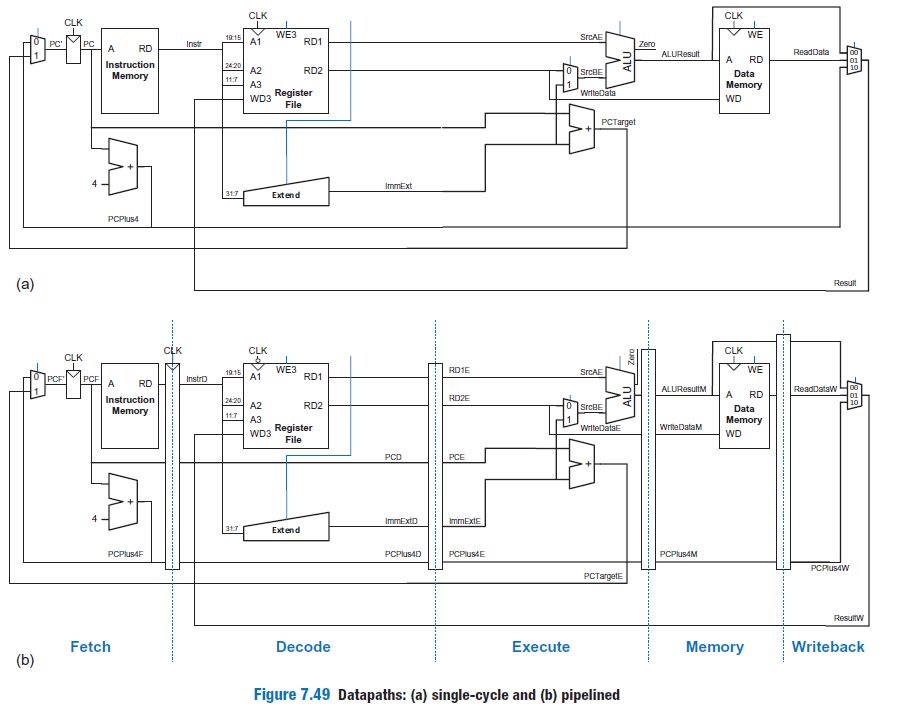
\includegraphics[width=0.95\textwidth]{figures/fig7.49.png}
    \caption{Pipelined datapath (Harris Figure~7.49b). Four pipeline registers (vertical bars) separate the five stages. The register file is drawn in the Decode stage, but its write address (\texttt{RdW}) and write data (\texttt{ResultW}) come from the Writeback stage --- this feedback is the source of pipeline hazards.}
    \label{fig:pipeline-datapath}
\end{figure}

Two subtleties are critical:

\begin{itemize}
    \item The register file writes on the \textit{falling} edge of CLK (first half of the cycle) and is read on the rising edge (second half). This allows a result to be written by one instruction and read by the next within the same cycle without introducing a hazard.
    \item The destination register \texttt{Rd} must be \textit{pipelined through} the Execute, Memory, and Writeback stages so it stays synchronised with the instruction's data. If \texttt{Rd} were taken from the Decode stage (as in the single-cycle processor), it would correspond to the wrong instruction.
\end{itemize}

\subsubsection{Control} The pipelined processor uses the same control unit as the single-cycle processor --- the same Main Decoder and ALU Decoder from Tables~\ref{tab:main-decoder} and~\ref{tab:alu-decoder}. The control signals are produced in the Decode stage and pipelined along with the data through subsequent stages. For example, \texttt{RegWriteD} becomes \texttt{RegWriteE} in Execute, \texttt{RegWriteM} in Memory, and \texttt{RegWriteW} in Writeback, where it finally enables the register file write.

\subsubsection{Hazards}

When multiple instructions execute simultaneously, dependencies arise that the hardware must resolve. These are classified as \textbf{data hazards} (an instruction needs a register value that a prior instruction has not yet written back) and \textbf{control hazards} (the branch decision has not been made by the time the next instruction must be fetched). A dedicated \textbf{Hazard Unit} detects these situations and resolves them using three mechanisms: forwarding, stalling, and flushing.

\paragraph{Solving data hazards with forwarding.} A \textit{read after write} (RAW) hazard occurs when an instruction in the Execute stage reads a register that a preceding instruction has not yet written back, hence reading the stale value. \textbf{Forwarding} (also called bypassing) solves this by routing the result directly from a later pipeline stage (Memory or Writeback) to the ALU inputs in Execute, bypassing the register file entirely. The hardware cost is two 3:1 forwarding multiplexers in front of the ALU, selecting each operand from: (00)~the register file output, (01)~\texttt{ResultW} from the Writeback stage, or (10)~\texttt{ALUResultM} from the Memory stage. The Hazard Unit compares the source registers of the instruction in Execute (\texttt{Rs1E}, \texttt{Rs2E}) against the destination registers in Memory and Writeback (\texttt{RdM}, \texttt{RdW}) to determine which input to select:

\begin{verbatim}
    if   ((Rs1E == RdM) & RegWriteM & (Rs1E != 0))  ForwardAE = 10  // Memory
    elif ((Rs1E == RdW) & RegWriteW & (Rs1E != 0))  ForwardAE = 01  // Writeback
    else                                            ForwardAE = 00  // Register file
\end{verbatim}

The logic for \texttt{ForwardBE} (the second ALU operand) is identical but checks \texttt{Rs2E}. The Memory stage has priority over Writeback because it contains the more recently executed instruction. Register \texttt{x0} is never forwarded because it is hardwired to zero.

\paragraph{Solving data hazards with stalls.} Forwarding works when the result is computed in the Execute stage, because it can be forwarded from Memory to the next instruction's Execute. But \texttt{lw} does not produce its result until the end of the Memory stage (when data memory is read), so the result cannot be forwarded to an instruction that needs it in the same cycle's Execute stage. This is a \textbf{load-use hazard}: \texttt{lw} has a two-cycle latency. The solution is to \textit{stall} the pipeline for one cycle, inserting a \textit{bubble} (a do-nothing cycle that propagates through the pipeline like a \texttt{nop}). The Fetch and Decode pipeline registers are held (\texttt{EN}=0, freezing their contents), and the Execute pipeline register is cleared (\texttt{CLR}=1, zeroing all control signals). After the stall, the \texttt{lw} result has reached the Writeback stage and can be forwarded normally. The stall condition is: $\texttt{lwStall} = \texttt{ResultSrcE}_0 \;\mathbin{\&}\; \bigl((\texttt{Rs1D} = \texttt{RdE}) \mathbin{|} (\texttt{Rs2D} = \texttt{RdE})\bigr)$ where $\texttt{ResultSrcE}_0 = 1$ indicates a load word is in the Execute stage.

\paragraph{Solving control hazards with flushing.} The \texttt{beq} instruction presents a control hazard: the branch decision (\texttt{PCSrcE}) is not computed until the Execute stage, by which time two subsequent instructions have already been fetched into the Decode and Execute stages. The simplest strategy is \textbf{predict not-taken}: the processor continues fetching sequentially and, if the branch turns out to be taken, \textit{flushes} (discards) the two incorrectly fetched instructions by clearing their pipeline registers (\texttt{CLR}=1). This incurs a 2-cycle misprediction penalty on every taken branch.

\paragraph{Hazard summary.} Figure~\ref{fig:pipeline-hazards} shows the complete pipelined processor with the Hazard Unit. The full hazard logic is:

\begin{center}\small
\renewcommand{\arraystretch}{1.15}
\begin{tabular}{@{}l l@{}}
    \toprule
    Signal & Logic \\
    \midrule
    \texttt{ForwardAE} & \texttt{10} if \texttt{(Rs1E==RdM) \& RegWriteM \& (Rs1E!=0)}; \\
    & \texttt{01} if \texttt{(Rs1E==RdW) \& RegWriteW \& (Rs1E!=0)}; else \texttt{00} \\
    \texttt{lwStall} & \texttt{ResultSrcE$_0$ \& ((Rs1D==RdE) | (Rs2D==RdE))} \\
    \texttt{StallF, StallD} & \texttt{lwStall} \\
    \texttt{FlushD} & \texttt{PCSrcE} \\
    \texttt{FlushE} & \texttt{lwStall | PCSrcE} \\
    \bottomrule
\end{tabular}
\end{center}

\begin{figure}[htbp]
    \centering
    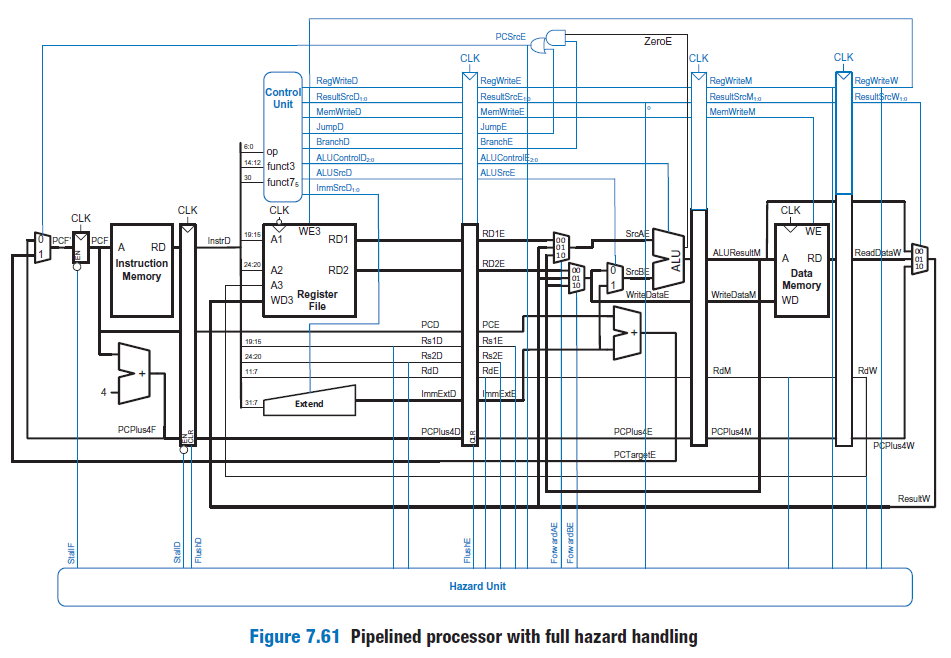
\includegraphics[width=0.95\textwidth]{figures/fig7.61.png}
    \caption{Complete pipelined RISC-V processor with full hazard handling (Harris Figure~7.61). The Hazard Unit (bottom) receives source registers from Execute (\texttt{Rs1E}, \texttt{Rs2E}) and destination registers from Memory and Writeback (\texttt{RdM}, \texttt{RdW}) to compute forwarding signals. It also receives \texttt{ResultSrcE$_0$} and \texttt{PCSrcE} to compute stall and flush signals. Compare with the single-cycle processor (Figure~\ref{fig:single-cycle-detail}): the pipeline adds four pipeline registers (vertical bars between stages), two forwarding multiplexers (3:1 muxes before the ALU), and enable/clear inputs on the pipeline registers for stall/flush control.}
    \label{fig:pipeline-hazards}
\end{figure}

\subsubsection{Critical path} The cycle time is set by the slowest of the five pipeline stages. Each stage's critical path must also account for pipeline register sequencing overhead ($t_{\text{pcq}}$ and $t_{\text{setup}}$). The Decode and Writeback stages use the register file in half-cycles (write on falling edge, read on rising edge), so twice their critical path must fit in one cycle:

$$
T_{c,\text{pipe}} = \max\!\begin{cases}
    t_{\text{pcq}} + t_{\text{mem}} + t_{\text{setup}} & \text{Fetch} \\
    2(t_{\text{RFread}} + t_{\text{setup}}) & \text{Decode} \\
    t_{\text{pcq}} + 4\,t_{\text{mux}} + t_{\text{ALU}} + t_{\text{AND-OR}} + t_{\text{setup}} & \text{Execute} \\
    t_{\text{pcq}} + t_{\text{mem}} + t_{\text{setup}} & \text{Memory} \\
    2(t_{\text{pcq}} + t_{\text{mux}} + t_{\text{RFsetup}}) & \text{Writeback}
\end{cases}
$$

The Execute stage is the bottleneck: its critical path includes the forwarding mux chain (Result mux $\to$ ForwardBE mux $\to$ SrcB mux), the ALU, and the AND-OR logic that computes \texttt{PCSrcE} from \texttt{BranchE \& ZeroE | JumpE}.

The CPI is ideally 1 but increases due to hazard penalties: load-use stalls add 1 cycle per dependent load, and branch mispredictions flush 2 cycles per taken branch. With a realistic instruction mix (SPECINT2000), average CPI\,$\approx$\,1.25. With 7\,nm delays, $T_{c,\text{pipe}} = 350$\,ps (limited by the Execute stage), giving $1.7\times$ speedup over single-cycle despite being far from the ideal $5\times$ (Table~\ref{tab:microarch-compare}). The gap comes from unbalanced stages and sequencing overhead paid on every stage. The hardware cost is pipeline registers, forwarding multiplexers, and the Hazard Unit.

\begin{figure}[htbp]
    \centering
    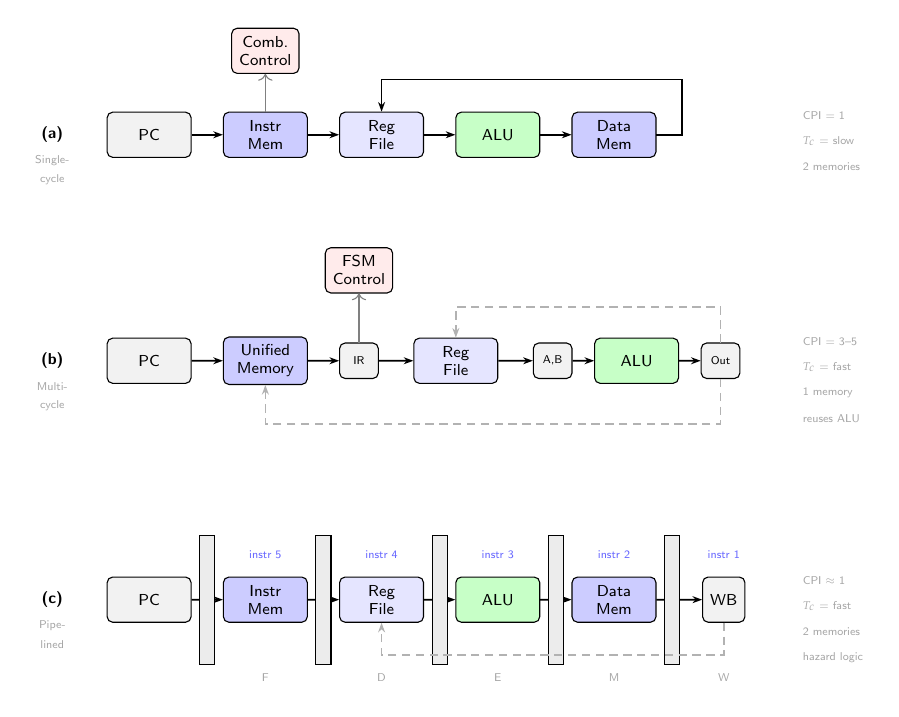
\begin{tikzpicture}[
      scale=0.82, every node/.style={transform shape},
      blk/.style={draw, rounded corners=2pt, minimum height=0.7cm,
                  minimum width=1.3cm, font=\sffamily\scriptsize, align=center},
      mem/.style={blk, fill=blue!20},
      reg/.style={blk, fill=blue!10},
      alu/.style={blk, fill=green!22},
      ctl/.style={blk, fill=red!8, minimum width=1.0cm},
      arr/.style={-{Stealth[length=3.5pt, width=2.5pt]}, semithick},
      lbl/.style={font=\sffamily\scriptsize\bfseries},
      note/.style={font=\sffamily\tiny, text=gray!70},
      pipereg/.style={draw, fill=gray!15, minimum width=0.12cm, minimum height=2.0cm},
      crit/.style={draw=red!50, line width=1.5pt, dashed}]

    % ============================================
    % (a) Single-cycle
    % ============================================
    \node[lbl] at (-1.5, 0) {(a)};
    \node[note] at (-1.5, -0.4) {Single-};
    \node[note] at (-1.5, -0.7) {cycle};

    \node[blk, fill=gray!10] (pc1) at (0, 0) {PC};
    \node[mem] (im1) at (1.8, 0) {Instr\\Mem};
    \node[reg] (rf1) at (3.6, 0) {Reg\\File};
    \node[alu] (alu1) at (5.4, 0) {ALU};
    \node[mem] (dm1) at (7.2, 0) {Data\\Mem};

    \draw[arr] (pc1) -- (im1);
    \draw[arr] (im1) -- (rf1);
    \draw[arr] (rf1) -- (alu1);
    \draw[arr] (alu1) -- (dm1);
    \draw[arr] (dm1.east) -- ++(0.4,0) |- ([yshift=0.5cm]rf1.north) -- (rf1.north);

    \node[ctl] (ctrl1) at (1.8, 1.3) {Comb.\\Control};
    \draw[->, gray, thin] (im1.north) -- (ctrl1.south);

    \node[note, anchor=west] at (10.0, 0.3) {CPI = 1};
    \node[note, anchor=west] at (10.0, -0.1) {$T_c$ = slow};
    \node[note, anchor=west] at (10.0, -0.5) {2 memories};

    % ============================================
    % (b) Multicycle
    % ============================================
    \def\yy{-3.5}
    \node[lbl] at (-1.5, \yy) {(b)};
    \node[note] at (-1.5, \yy-0.4) {Multi-};
    \node[note] at (-1.5, \yy-0.7) {cycle};

    \node[blk, fill=gray!10] (pc2) at (0, \yy) {PC};
    \node[mem] (um2) at (1.8, \yy) {Unified\\Memory};
    \node[blk, fill=gray!10, minimum width=0.6cm, minimum height=0.55cm, font=\sffamily\tiny] (ir2) at (3.25, \yy) {IR};
    \node[reg] (rf2) at (4.75, \yy) {Reg\\File};
    \node[blk, fill=gray!10, minimum width=0.6cm, minimum height=0.55cm, font=\sffamily\tiny] (ab2) at (6.25, \yy) {A,B};
    \node[alu] (alu2) at (7.55, \yy) {ALU};
    \node[blk, fill=gray!10, minimum width=0.6cm, minimum height=0.55cm, font=\sffamily\tiny] (ao2) at (8.85, \yy) {Out};

    \draw[arr] (pc2) -- (um2);
    \draw[arr] (um2) -- (ir2);
    \draw[arr] (ir2) -- (rf2);
    \draw[arr] (rf2) -- (ab2);
    \draw[arr] (ab2) -- (alu2);
    \draw[arr] (alu2) -- (ao2);

    % reuse arrows (ALU back to memory, result back to regfile)
    \draw[arr, gray!60, densely dashed] (ao2.south) -- ++(0,-0.7) -| (um2.south);
    \draw[arr, gray!60, densely dashed] (ao2.north) -- ++(0,0.55) -| (rf2.north);

    \node[ctl] (ctrl2) at (3.25, \yy+1.4) {FSM\\Control};
    \draw[->, gray, thin] (ir2.north) -- (ctrl2.south);

    \node[note, anchor=west] at (10.0, \yy+0.3) {CPI = 3--5};
    \node[note, anchor=west] at (10.0, \yy-0.1) {$T_c$ = fast};
    \node[note, anchor=west] at (10.0, \yy-0.5) {1 memory};
    \node[note, anchor=west] at (10.0, \yy-0.9) {reuses ALU};

    % ============================================
    % (c) Pipelined
    % ============================================
    \def\yyy{-7.2}
    \node[lbl] at (-1.5, \yyy) {(c)};
    \node[note] at (-1.5, \yyy-0.4) {Pipe-};
    \node[note] at (-1.5, \yyy-0.7) {lined};

    \node[blk, fill=gray!10] (pc3) at (0, \yyy) {PC};
    \node[mem] (im3) at (1.8, \yyy) {Instr\\Mem};
    \node[reg] (rf3) at (3.6, \yyy) {Reg\\File};
    \node[alu] (alu3) at (5.4, \yyy) {ALU};
    \node[mem] (dm3) at (7.2, \yyy) {Data\\Mem};
    \node[blk, fill=gray!10, minimum width=0.6cm] (wb3) at (8.9, \yyy) {WB};

    \draw[arr] (pc3) -- (im3);
    \draw[arr] (im3) -- (rf3);
    \draw[arr] (rf3) -- (alu3);
    \draw[arr] (alu3) -- (dm3);
    \draw[arr] (dm3) -- (wb3);

    % Pipeline register bars (centered between blocks)
    \foreach \x in {0.9, 2.7, 4.5, 6.3, 8.1} {
        \node[pipereg] at (\x, \yyy) {};
    }

    % Stage labels (centered in each stage region between pipeline registers)
    \node[note] at (1.8, \yyy-1.2) {F};
    \node[note] at (3.6, \yyy-1.2) {D};
    \node[note] at (5.4, \yyy-1.2) {E};
    \node[note] at (7.2, \yyy-1.2) {M};
    \node[note] at (8.9, \yyy-1.2) {W};

    % Multiple instructions in flight (one per stage)
    \node[note, text=blue!60] at (1.8, \yyy+0.7) {instr 5};
    \node[note, text=blue!60] at (3.6, \yyy+0.7) {instr 4};
    \node[note, text=blue!60] at (5.4, \yyy+0.7) {instr 3};
    \node[note, text=blue!60] at (7.2, \yyy+0.7) {instr 2};
    \node[note, text=blue!60] at (8.9, \yyy+0.7) {instr 1};

    \draw[arr, gray!60, densely dashed] (wb3.south) -- ++(0,-0.5) -| (rf3.south);

    \node[note, anchor=west] at (10.0, \yyy+0.3) {CPI $\approx$ 1};
    \node[note, anchor=west] at (10.0, \yyy-0.1) {$T_c$ = fast};
    \node[note, anchor=west] at (10.0, \yyy-0.5) {2 memories};
    \node[note, anchor=west] at (10.0, \yyy-0.9) {hazard logic};

    \end{tikzpicture}
    \caption{Three microarchitecture styles, compared below. For full datapaths with all control signals, see Harris Figures~7.12, 7.27, and~7.61.}
    \label{fig:microarch-compare}
\end{figure}

\subsection{Summary}

The three architectures in Figure~\ref{fig:microarch-compare} differ in how they connect the same building blocks:

\begin{itemize}
    \item \textbf{(a) Single-cycle}: data flows left-to-right through the entire datapath in one clock cycle. The critical path spans PC $\to$ instruction memory $\to$ register file $\to$ ALU $\to$ data memory $\to$ writeback (red dashed line), so $T_c$ is long. CPI\,=\,1, but the clock is slow. Requires two separate memories (instruction and data, since both are read in the same cycle) and three adders (ALU + two for PC logic). The controller is purely combinational --- a truth table from opcode to control signals.

    \item \textbf{(b) Multicycle}: the same hardware is reused across multiple shorter cycles. A single unified memory serves both instructions and data (accessed on different cycles), and a single ALU handles arithmetic, address calculation, and PC+4 (on different cycles). The dashed feedback arrows show data cycling back: ALU output feeds back to the memory address input and to the register file. Nonarchitectural registers (IR, A, B, Out) hold intermediate results between steps. The controller is an FSM that produces different control signals on each step. $T_c$ is fast (set by a single memory access or ALU operation), but CPI\,=\,3--5.

    \item \textbf{(c) Pipelined}: the single-cycle datapath is chopped into five stages by inserting pipeline registers (grey bars). Five instructions execute simultaneously, one in each stage (labelled F, D, E, M, W). Like the single-cycle design, it needs two memories and has CPI\,$\approx$\,1, but $T_c$ is set by the slowest \emph{stage} rather than the entire datapath. The cost is hazard logic: forwarding multiplexers, stall/flush signals, and a Hazard Unit to handle data and control dependencies between instructions in different stages.
\end{itemize}

Harris Example~7.10 compares the three architectures executing $10^{11}$ instructions:

\begin{table}[htbp]
\centering\small
\begin{tabular}{@{}l c c c c@{}}
    \toprule
    & CPI & $T_c$ (ps) & $T_{\text{exec}}$ (s) & Memories \\
    \midrule
    Single-cycle & 1 & 750 & 75 & 2 (separate I/D) \\
    Multicycle & 4.14 & 375 & 155 & 1 (shared) \\
    Pipelined & 1.25 & 350 & 44 & 2 (I/D caches) \\
    \bottomrule
\end{tabular}
\caption{Performance comparison of three microarchitectures (Harris Example~7.10, 7\,nm CMOS delays).}
\label{tab:microarch-compare}
\end{table}

The multicycle processor is actually the \emph{slowest} here because its high CPI (4.14) overwhelms its shorter $T_c$. The pipelined processor wins with 1.7$\times$ speedup over single-cycle. But the multicycle design uses the \emph{least hardware} (one memory, one ALU, no pipeline registers, no hazard unit), which matters when the FPGA has only 5280 LUTs.

\subsection{Advanced microarchitecture techniques}

Beyond the three basic microarchitectures, high-performance processors use additional techniques to increase throughput. Harris~\S7.7 surveys these; the most relevant to ML accelerator design are summarised here.

\paragraph{Superscalar processors (spatial parallelism).} A superscalar processor contains multiple copies of the datapath hardware to execute multiple instructions per cycle. A two-way superscalar fetches two instructions, reads four source operands from a six-ported register file, executes on two ALUs, and writes two results --- achieving IPC\,$>$\,1 on code without dependencies. Commercial processors are three- to six-way superscalar, but real programs have enough dependencies that the execution units are rarely fully utilised. GPUs take this idea to the extreme: thousands of simple cores executing the same instruction on different data (SIMT).

\paragraph{Multiprocessing and multithreading.} \textbf{Multiprocessing} places multiple independent processor cores on a single chip, each with its own datapath and control unit. Each core can run a separate program simultaneously. A quad-core CPU has four complete processors sharing main memory; coordination between cores uses shared-memory protocols (cache coherence) or message passing.

\textbf{Hardware multithreading} is a different idea: a \emph{single} core replicates only the architectural state (PC + register file) so multiple threads are resident simultaneously, but they \emph{share} the datapath hardware (ALU, memory interface). When one thread stalls on a slow memory access, the core immediately switches to another thread whose registers are already loaded --- no context-switch penalty. The datapath stays busy even though individual threads are waiting. \textit{fine-grained} multithreading switches threads every cycle (round-robin), smoothing out short stalls; \textit{coarse-grained} switches only on expensive stalls like cache misses, avoiding the per-cycle switching overhead. \textbf{Simultaneous multithreading} (SMT, marketed as Intel Hyper-Threading) goes further: multiple threads issue instructions to the \emph{same} execution units in the \emph{same} cycle, filling bubbles left by dependencies in each individual thread.

The key distinction: multiprocessing duplicates entire cores (more hardware, true parallel execution); multithreading duplicates only state (less hardware, hides latency by interleaving). GPUs combine both: thousands of simple cores, each running many hardware threads (warps), to hide the long latency of DRAM accesses.

\paragraph{Hardware accelerators.} Rather than adding more identical cores, a system can incorporate specialised hardware (accelerators) optimised for specific tasks. Accelerators can be 10--100$\times$ more efficient in performance, cost, and power than general-purpose cores for the same computation. Examples include GPU shader cores for graphics, DSPs for signal processing, and TPU-style systolic arrays for matrix multiply. The CPU handles control flow and data movement; the accelerator handles the data-parallel inner loop.

\subsection{Where picorv32 fits}

Regardless of microarchitecture, a processor presents the same external interface: address and data busses to instruction and data memories, plus clock and reset. Figure~\ref{fig:proc-interface} shows this for the single-cycle case --- the Controller and Datapath are encapsulated in a module that communicates with external memories through well-defined ports (PC, Instr, DataAdr, WriteData, ReadData). A multicycle or pipelined processor has a different internal organisation but exposes the same kind of interface. picorv32 follows this pattern, replacing the direct address/data busses with a valid/ready handshake (\texttt{mem\_valid}/\texttt{mem\_ready}).

\begin{figure}[htbp]
    \centering
    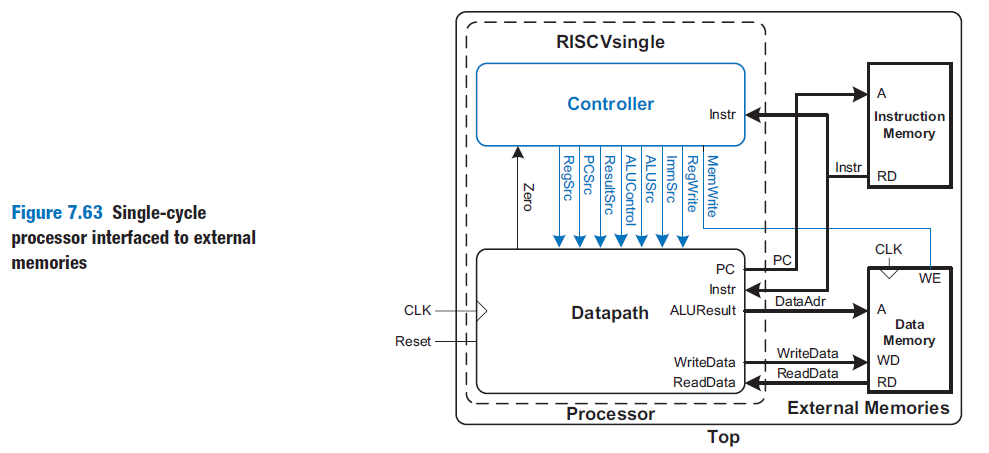
\includegraphics[width=0.75\textwidth]{figures/fig7.63.png}
    \caption{Single-cycle processor interfaced to external memories (Harris Figure~7.63). The processor module contains a Controller and Datapath; it communicates with separate Instruction and Data memories through address, data, and control busses. Any microarchitecture (single-cycle, multicycle, pipelined) presents a similar external interface --- only the internal organisation differs.}
    \label{fig:proc-interface}
\end{figure}

The picorv32 is a multicycle design --- it uses a single memory interface, an FSM controller, and nonarchitectural registers --- but it departs from the textbook in several ways:

\begin{itemize}
    \item \textit{One-hot state encoding}: 8 states in an 8-bit register (\texttt{cpu\_state[7:0]}), each state a single bit. This synthesises to fast parallel-case logic on FPGAs, unlike the textbook's binary-encoded FSM.
    \item \textit{No dedicated decode state}: the textbook multicycle FSM has a Decode state that reads registers and computes the branch target address. picorv32 merges this into \texttt{cpu\_state\_ld\_rs1}, saving one cycle on most instructions.
    \item \textit{Configurable datapath}: parameters like \texttt{BARREL\_SHIFTER}, \texttt{TWO\_CYCLE\_ALU}, \texttt{TWO\_STAGE\_SHIFT} let the user trade LUTs for speed. Without a barrel shifter, shifts take 1--32 extra cycles; with one, they complete in the ALU combinationally.
    \item \textit{Look-ahead memory interface}: the \texttt{mem\_la\_*} signals allow memory to begin responding before the bus handshake is formally asserted, partially overlapping fetch with decode.
    \item \textit{PCPI co-processor port}: unrecognised instructions are forwarded to external hardware, enabling multiply/divide without enlarging the core.
\end{itemize}

\newpage

\section{Memory Systems}
\label{sec:memory}

\begin{comment}
READ: Harris Ch 8 (§8.1 Introduction, §8.2 Performance Analysis, §8.3 Caches, §8.4 Virtual Memory)
SCREENSHOTS: fig8.5.png (memory-to-cache mapping), fig8.7.png (direct mapped hardware),
  fig8.9.png (2-way set associative hardware), fig8.12.png (4-word block size cache)
TIKZ: memory hierarchy diagram, address field breakdowns (Fig 8.6 / 8.13 style)
\end{comment}

Chapter~7 assumed an ideal memory that could be accessed in a single clock cycle. In reality, DRAM is 10--100$\times$ slower than the processor. Memory systems bridge this gap using a hierarchy of progressively larger, slower, cheaper storage, exploiting the locality of real programs to make the common case fast.

\subsection{The Memory Hierarchy}

Memory speed is much slower than processor speed. DRAM throughput is reasonable ($\sim$30\,GB/s), but latency is the bottleneck. The solution exploits two empirical principles:

\begin{itemize}
    \item \textbf{Temporal locality}: if a piece of data was accessed recently, it is likely to be accessed again soon. (A variable used in a loop is reused every iteration.)
    \item \textbf{Spatial locality}: if a piece of data was accessed, nearby data is likely to be accessed soon. (Consecutive array elements are stored at consecutive addresses.)
\end{itemize}

By keeping recently and nearby used data in a small, fast memory (a \textbf{cache}, built from on-chip SRAM), and storing the rest in large, slow main memory (DRAM) or an even larger hard drive, the system approximates a memory that is simultaneously fast, large, and cheap. Figure~\ref{fig:mem-hierarchy} shows the hierarchy with representative 2021 characteristics.

\begin{table}[htbp]
\centering\small
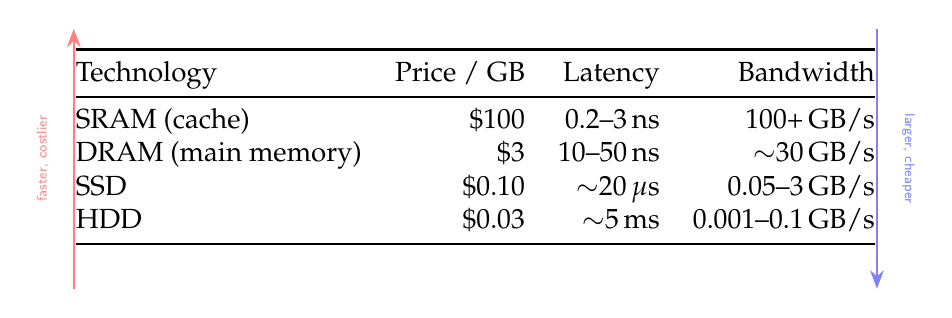
\begin{tikzpicture}[>=Stealth]
  % Left arrow: speed (upward)
  \draw[->, red!50, thick] (-0.4, -1.8) -- (-0.4, 1.5);
  \node[font=\sffamily\tiny, text=red!50, rotate=90, anchor=south] at (-0.6, -0.15) {faster, costlier};
  % Right arrow: capacity (downward)
  \draw[->, blue!50, thick] (9.8, 1.5) -- (9.8, -1.8);
  \node[font=\sffamily\tiny, text=blue!50, rotate=-90, anchor=south] at (10.0, -0.15) {larger, cheaper};
  % Table
  \node at (4.7, 0) {
    \begin{tabular}{@{}l r r r@{}}
      \toprule
      Technology & Price / GB & Latency & Bandwidth \\
      \midrule
      SRAM (cache)        & \$100  & 0.2--3\,ns       & 100+\,GB/s \\
      DRAM (main memory)  & \$3    & 10--50\,ns       & $\sim$30\,GB/s \\
      SSD                 & \$0.10 & $\sim$20\,$\mu$s  & 0.05--3\,GB/s \\
      HDD                 & \$0.03 & $\sim$5\,ms       & 0.001--0.1\,GB/s \\
      \bottomrule
    \end{tabular}
  };
\end{tikzpicture}
\caption{Memory hierarchy (after Harris Figure~8.3, Table~8.1). Each level is roughly 10$\times$ slower and 10--30$\times$ cheaper per GB than the one above. The processor seeks data in the cache first; on a miss, it falls through to main memory, then to disk.}
\label{fig:mem-hierarchy}
\end{table}

If the processor requests data that is available in the cache, it is returned quickly --- a \textbf{cache hit}. Otherwise, the data must be fetched from main memory --- a \textbf{cache miss}. If the cache hits most of the time, the average access time approaches the cache speed rather than the DRAM speed. The hard drive provides \textbf{virtual memory}: an illusion of more capacity than physically exists in DRAM. Main memory acts as a cache for the hard drive, just as the cache acts as a cache for main memory.

\subsection{Memory System Performance Analysis}

The key metrics are \textbf{miss rate} (or equivalently hit rate) and \textbf{average memory access time} (AMAT):

$$
\text{Miss Rate} = \frac{\text{Number of misses}}{\text{Total memory accesses}} = 1 - \text{Hit Rate}
$$

$$
\text{AMAT} = t_{\text{cache}} + \text{MR}_{\text{cache}}\!\left(t_{\text{MM}} + \text{MR}_{\text{MM}} \cdot t_{\text{VM}}\right)
$$

where $t_{\text{cache}}$, $t_{\text{MM}}$, $t_{\text{VM}}$ are the access times of the cache, main memory, and virtual memory, and $\text{MR}_{\text{cache}}$, $\text{MR}_{\text{MM}}$ are their miss rates. For a two-level system (cache + main memory only), this simplifies to $\text{AMAT} = t_{\text{cache}} + \text{MR}_{\text{cache}} \cdot t_{\text{MM}}$.

\paragraph{Amdahl's Law.} Improving one subsystem yields diminishing returns if that subsystem is not the dominant bottleneck. If 50\% of instructions are loads/stores, making memory 10$\times$ faster improves overall performance by only $1/(0.5 + 0.5/10) = 1.82\times$. The effort spent increasing a subsystem's performance is worthwhile only if that subsystem affects a large fraction of the overall execution time.

\subsection{Caches}
\label{sec:caches}

A cache holds a subset of main memory's data. It is specified by five parameters:

\begin{itemize}
    \item \textbf{Capacity} $C$: total number of data words the cache can hold.
    \item \textbf{Block size} $b$: number of words per cache block (also called a cache line). A block is the unit of transfer between cache and main memory.
    \item \textbf{Number of blocks} $B = C / b$.
    \item \textbf{Associativity} $N$: number of blocks in each set (i.e., how many places a given address can map to).
    \item \textbf{Number of sets} $S = B / N$.
\end{itemize}

\subsubsection{What Data is Held in the Cache?}

The cache exploits both forms of locality:

\begin{itemize}
    \item \textbf{Temporal locality}: when the processor loads or stores data not in the cache, that data is copied from main memory into the cache. Subsequent accesses to the same address hit in the cache.
    \item \textbf{Spatial locality}: when a cache miss occurs, the cache fetches not just the requested word but an entire \textbf{block} of $b$ adjacent words. Subsequent accesses to nearby addresses are likely to hit because the neighbouring words are already in the cache.
\end{itemize}

If a program accessed data in a purely random order, a cache would provide no benefit. But real programs have strong locality --- variables are reused in loops (temporal), and array elements are accessed sequentially (spatial).

\subsubsection{How is Data Found?}

The cache is organised as a two-dimensional array: the rows are \textbf{sets} and the columns are \textbf{ways}. Each memory address maps to exactly one set (determined by some address bits), but within that set, the data can be stored in any of the $N$ ways.

% Shared TikZ styles for cache mapping diagrams
\tikzset{
  cmem/.style={draw, minimum width=1.6cm, minimum height=0.4cm,
               font=\sffamily\tiny, inner sep=1pt, align=center},
  ccache/.style={draw, minimum width=1.4cm, minimum height=0.4cm,
                 font=\sffamily\tiny, inner sep=1pt, align=center},
  chdr/.style={font=\sffamily\tiny\bfseries},
  caddr/.style={font=\ttfamily\tiny, text=gray!60},
  csub/.style={font=\sffamily\tiny, text=gray},
  carr/.style={->, gray!40, thin}
}

\paragraph{Direct mapped cache.} A direct mapped cache has $N = 1$ (one block per set, so $S = B$). Each address maps to a \emph{unique} location in the cache. Figure~\ref{fig:cache-dm-map} shows the mapping for an 8-word cache (8 sets) with $b = 1$: the bottom two bits of the address are always 00 (word-aligned\footnote{\textbf{Word-aligned} means the address is a multiple of 4 (the word size in bytes), so bits [1:0] are always \texttt{00}. This ensures a 32-bit word is read in a single memory access. Since memory is byte-addressed, a 32-bit word spans 4 consecutive byte addresses.}); the next $\log_2 8 = 3$ bits select the set; higher addresses wrap around, so addresses 0x04, 0x24, 0x44, \ldots\ all map to set~1.

\begin{figure}[htbp]
    \centering
    \begin{tikzpicture}[>=Stealth, semithick, scale=0.85, every node/.style={transform shape}]
    \def\rh{0.48}
    % Parameters
    \node[draw, rounded corners=2pt, fill=gray!5, font=\sffamily\tiny, align=left, anchor=north west]
      at (9.5, 0.5) {$C\!=\!4$, $b\!=\!1$, $B\!=\!4$\\$N\!=\!1$, $S\!=\!4$};
    % Memory with binary addresses
    \node[chdr] at (1.0, 0.5) {tag$\vert$set$\vert$byte};
    \foreach \i/\bin in {0/{0\textbar 00\textbar 00}, 1/{0\textbar 01\textbar 00},
                          2/{0\textbar 10\textbar 00}, 3/{0\textbar 11\textbar 00},
                          4/{1\textbar 00\textbar 00}, 5/{1\textbar 01\textbar 00},
                          6/{1\textbar 10\textbar 00}, 7/{1\textbar 11\textbar 00}} {
        \pgfmathtruncatemacro{\s}{mod(\i,4)}
        \ifcase\s \def\col{red!10}\or \def\col{blue!10}\or \def\col{green!8}\or \def\col{orange!8}\fi
        \node[cmem, fill=\col, font=\ttfamily\tiny] (ma\i) at (1.0, -\i*\rh) {\bin};
    }
    \node[chdr] at (1.0, -7*\rh-0.4) {Memory};
    % Cache
    \node[chdr] at (6.5, 0.5) {V};
    \node[chdr] at (7.2, 0.5) {Tag};
    \node[chdr] at (8.2, 0.5) {Data};
    \foreach \s/\col in {0/red!10, 1/blue!10, 2/green!8, 3/orange!8} {
        \node[ccache, fill=\col, minimum width=0.4cm] (dv\s) at (6.5, -\s*\rh) {};
        \node[ccache, fill=\col, minimum width=1.0cm] at (7.2, -\s*\rh) {};
        \node[ccache, fill=\col, minimum width=1.2cm] at (8.2, -\s*\rh) {};
        \node[csub, anchor=west] at (8.9, -\s*\rh) {Set \s};
    }
    \foreach \i in {0,...,7} {
        \pgfmathtruncatemacro{\s}{mod(\i,4)}
        \draw[carr] (ma\i.east) -- (dv\s.west);
    }
    \node[chdr] at (7.5, -3*\rh-0.4) {Cache};
    \node[csub, align=center, anchor=north west] at (6.5, -2.2) {block $i \to$ set ($i$ mod 4)\\each set holds \emph{one} block};
    \end{tikzpicture}
    \caption{Direct mapped cache ($N\!=\!1$, $S\!=\!4$). Binary addresses show \texttt{tag|set|byte} fields; blocks with the same set bits (e.g.\ 0 and 4, both \texttt{00}) conflict.}
    \label{fig:cache-dm-map}
\end{figure}

Because many addresses map to the same set, the cache must record \emph{which} address is actually stored there. The main memory address is broken down into three fields:

\begin{center}
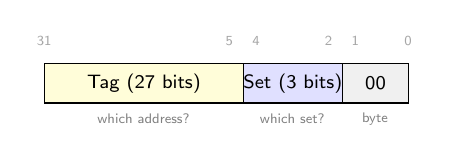
\begin{tikzpicture}[
  every node/.style={transform shape},
  fld/.style={draw, minimum height=0.5cm, inner sep=0pt,
              font=\sffamily\scriptsize, text centered},
  bit/.style={font=\sffamily\tiny\color{gray!70}, anchor=south}]

  \def\bp{0.42}

  % Field widths: Tag[31:5]=6bp, Set[4:2]=3bp, Byte[1:0]=2bp → total 11bp
  % Boundaries at x = 0, 6bp, 9bp, 11bp

  % Bit labels at field boundaries (pairs offset at shared edges)
  \node[bit] at (0, 0.35) {31};
  \node[bit, anchor=south east] at (6*\bp, 0.35) {5};
  \node[bit, anchor=south west] at (6*\bp, 0.35) {4};
  \node[bit, anchor=south east] at (9*\bp, 0.35) {2};
  \node[bit, anchor=south west] at (9*\bp, 0.35) {1};
  \node[bit] at (11*\bp, 0.35) {0};

  % Fields
  \node[fld, fill=yellow!15, minimum width=6*\bp cm, anchor=west] at (0, 0) {Tag (27 bits)};
  \node[fld, fill=blue!12, minimum width=3*\bp cm, anchor=west] at (6*\bp, 0) {Set (3 bits)};
  \node[fld, fill=gray!12, minimum width=2*\bp cm, anchor=west] at (9*\bp, 0) {00};

  % Labels below (centered under each field)
  \node[font=\sffamily\tiny, text=gray] at (3*\bp, -0.45) {which address?};
  \node[font=\sffamily\tiny, text=gray] at (7.5*\bp, -0.45) {which set?};
  \node[font=\sffamily\tiny, text=gray] at (10*\bp, -0.45) {byte};

\end{tikzpicture}
\end{center}

The tag is only 27 bits, not the full 32-bit address, because the other 5 bits are already known: the set bits tell the hardware \emph{which row} it is reading, and the byte offset is implied by word alignment. Together, \texttt{\{tag, set, 00\}} reconstructs the full 32-bit address. Each set in the cache stores:

\begin{itemize}
    \item \textbf{Byte offset} [1:0]: always 00 for word-aligned accesses (selects the byte within the word). Not stored in the cache --- implicit.
    \item \textbf{Set bits} [$\log_2 S + 1 : 2$]: select which row in the cache SRAM to read. Not stored --- implicit from the row position.
    \item \textbf{Tag} [31 : $\log_2 S + 2$]: the remaining upper bits (27 in this example). Stored alongside the data so the cache can check whether the requested address matches what is actually held in this set.
    \item \textbf{Valid bit} $V$ (1 bit): is this entry holding real data? $V = 0$ after power-on means the entry is empty.
    \item \textbf{Data} ($b$ words): the actual cached data.
\end{itemize}

A \textbf{cache hit} occurs when $V = 1$ \emph{and} the stored tag matches the tag field of the requested address. Figure~\ref{fig:cache-dm-hw} shows the hardware: the set bits index an 8-entry SRAM of $(1 + 27 + 32)$-bit rows; the stored tag is compared with the address tag; if they match and $V = 1$, the data is returned.

\begin{figure}[htbp]
    \centering
    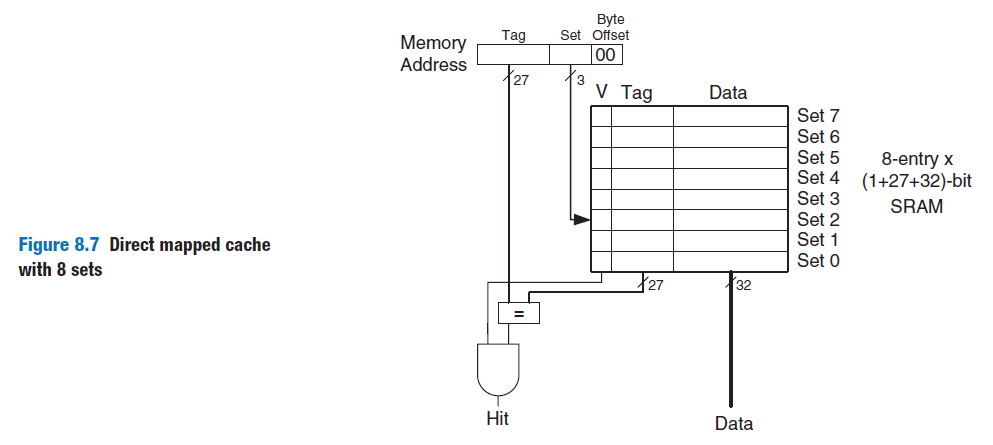
\includegraphics[width=0.55\textwidth]{figures/fig8.7.png}
    \caption{Direct mapped cache hardware (Harris Figure~8.7). The set bits index an 8-entry SRAM; the stored tag is compared with the address tag; if they match and $V = 1$, the cache hits and returns the data.}
    \label{fig:cache-dm-hw}
\end{figure}

\paragraph{Example: temporal locality (Harris 8.6).} Consider a loop that executes 5 iterations, each accessing addresses 0x4, 0xC, and 0x8 (mapping to sets 1, 3, 2). On the first iteration, the cache is empty: 3 misses. On iterations 2--5, all accesses hit. Miss rate = $3/15 = 20\%$.

\paragraph{Example: conflict misses (Harris 8.7).} Now consider a loop accessing addresses 0x4 and 0x24 --- both map to set~1. On every iteration, each access evicts the other. The miss rate is 100\%, even though the cache has 8 sets and only 2 are needed. This pathology is a \textbf{conflict miss}: two addresses compete for the same set.

\paragraph{Set associative cache.} An $N$-way set associative cache provides $N$ blocks per set ($S = B/N$), reducing conflicts. The address still maps to a unique set, but within that set, the data can occupy any of the $N$ ways. Figure~\ref{fig:cache-sa-map} shows the mapping for a 2-way cache: compared to direct-mapped, the number of sets halves (from 4 to 2) but each set can hold two blocks, so the total capacity is the same. The hardware reads all $N$ tags in the selected set simultaneously and checks for a match. Figure~\ref{fig:cache-sa-hw} shows the hardware for $C = 8$ words.

\begin{figure}[htbp]
    \centering
    \begin{tikzpicture}[>=Stealth, semithick, scale=0.85, every node/.style={transform shape}]
    \def\rh{0.48}
    % Parameters
    \node[draw, rounded corners=2pt, fill=gray!5, font=\sffamily\tiny, align=left, anchor=north west]
      at (10.0, 0.5) {$C\!=\!4$, $b\!=\!1$, $B\!=\!4$\\$N\!=\!2$, $S\!=\!2$};
    % Memory with binary addresses
    \node[chdr] at (1.0, 0.5) {tag$\vert$set$\vert$byte};
    \foreach \i/\bin in {0/{00\textbar 0\textbar 00}, 1/{00\textbar 1\textbar 00},
                          2/{01\textbar 0\textbar 00}, 3/{01\textbar 1\textbar 00},
                          4/{10\textbar 0\textbar 00}, 5/{10\textbar 1\textbar 00},
                          6/{11\textbar 0\textbar 00}, 7/{11\textbar 1\textbar 00}} {
        \pgfmathtruncatemacro{\s}{mod(\i,2)}
        \ifcase\s \def\col{red!10}\or \def\col{blue!10}\fi
        \node[cmem, fill=\col, font=\ttfamily\tiny] (mb\i) at (1.0, -\i*\rh) {\bin};
    }
    \node[chdr] at (1.0, -7*\rh-0.4) {Memory};
    % Cache
    \node[chdr] at (5.7, 0.5) {Way 0};
    \node[chdr] at (7.8, 0.5) {Way 1};
    \foreach \s/\col/\coll/\lbl in {0/red!10/red!5/Set 0, 1/blue!10/blue!5/Set 1} {
        \node[ccache, fill=\col, minimum width=0.35cm] at (5.2, -\s*\rh) {};
        \node[ccache, fill=\col, minimum width=0.7cm] at (5.7, -\s*\rh) {};
        \node[ccache, fill=\col, minimum width=0.9cm] (bw0s\s) at (6.5, -\s*\rh) {};
        \node[ccache, fill=\coll, minimum width=0.35cm] at (7.3, -\s*\rh) {};
        \node[ccache, fill=\coll, minimum width=0.7cm] at (7.8, -\s*\rh) {};
        \node[ccache, fill=\coll, minimum width=0.9cm] at (8.6, -\s*\rh) {};
        \node[csub, anchor=west] at (9.2, -\s*\rh) {\lbl};
    }
    \foreach \i in {0, 2, 4, 6} { \draw[carr] (mb\i.east) -- (bw0s0.west); }
    \foreach \i in {1, 3, 5, 7} { \draw[carr] (mb\i.east) -- (bw0s1.west); }
    \node[chdr] at (7.0, -1*\rh-0.4) {Cache};
    \node[csub, align=center, anchor=north west] at (5.2, -1.5) {block $i \to$ set ($i$ mod 2)\\each set holds \emph{two} blocks};
    \end{tikzpicture}
    \caption{2-way set associative cache ($N\!=\!2$, $S\!=\!2$). The set field is now 1 bit; the tag grows to 2 bits. Blocks 0 and 4 (both set bit \texttt{0}) coexist in different ways instead of conflicting.}
    \label{fig:cache-sa-map}
\end{figure}

\begin{figure}[htbp]
    \centering
    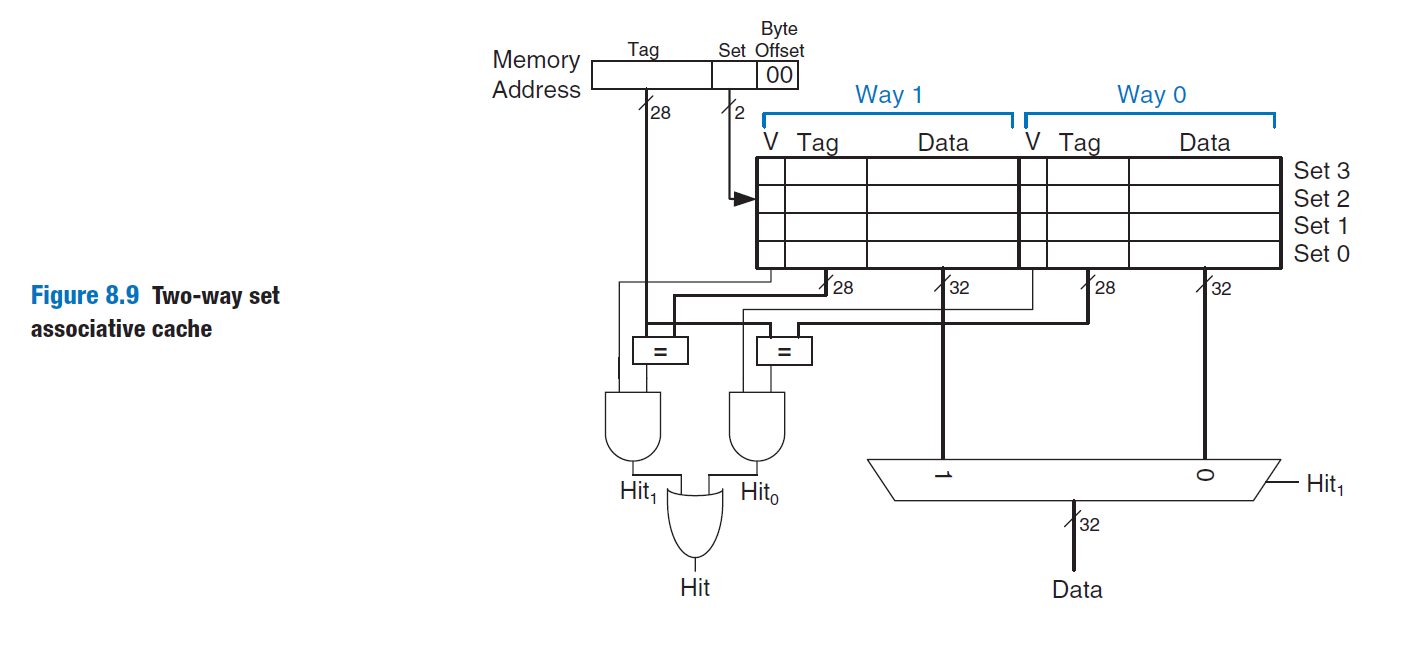
\includegraphics[width=0.55\textwidth]{figures/fig8.9.png}
    \caption{Two-way set associative cache hardware (Harris Figure~8.9). The cache has $S = 4$ sets (2 set bits instead of 3). Each set contains two ways, each with its own tag and valid bit. Both ways are read and compared in parallel; a multiplexer selects the data from the hitting way.}
    \label{fig:cache-sa-hw}
\end{figure}

With 2 ways, the conflict from the previous example disappears: addresses 0x4 and 0x24 both map to set~1, but they occupy different ways. The miss rate drops from 100\% to $2/10 = 20\%$ (2 compulsory misses on the first iteration, then all hits). Set associative caches generally have lower miss rates than direct mapped caches of the same capacity. The cost is $N$ tag comparators and an output multiplexer, making them slower and slightly larger. Most commercial systems use 4-way or 8-way set associative caches.

\paragraph{Fully associative cache.} A fully associative cache has $S = 1$ set and $B$ ways --- data can go in any block (Figure~\ref{fig:cache-fa-map}). This minimises conflict misses but requires $B$ comparators, making it practical only for very small caches (e.g.\ TLBs with 16--512 entries, Section~\ref{sec:vm}).

\begin{figure}[htbp]
    \centering
    \begin{tikzpicture}[>=Stealth, semithick, scale=0.85, every node/.style={transform shape}]
    \def\rh{0.48}
    % Parameters
    \node[draw, rounded corners=2pt, fill=gray!5, font=\sffamily\tiny, align=left, anchor=north west]
      at (13.5, 0.5) {$C\!=\!4$, $b\!=\!1$, $B\!=\!4$\\$N\!=\!4$, $S\!=\!1$};
    % Memory with binary addresses
    \node[chdr] at (1.0, 0.5) {tag$\vert$byte};
    \foreach \i/\bin in {0/{000\textbar 00}, 1/{001\textbar 00},
                          2/{010\textbar 00}, 3/{011\textbar 00},
                          4/{100\textbar 00}, 5/{101\textbar 00},
                          6/{110\textbar 00}, 7/{111\textbar 00}} {
        \node[cmem, fill=gray!8, font=\ttfamily\tiny] (mc\i) at (1.0, -\i*\rh) {\bin};
    }
    \node[chdr] at (1.0, -7*\rh-0.4) {Memory};
    % Cache
    \foreach \w/\lbl in {0/Way 0, 1/Way 1, 2/Way 2, 3/Way 3} {
        \pgfmathsetmacro{\cx}{5.2 + \w*2.05}
        \node[chdr] at (\cx+0.5, 0.5) {\lbl};
        \node[ccache, fill=gray!8, minimum width=0.35cm] at (\cx, 0) {};
        \node[ccache, fill=gray!8, minimum width=0.7cm] at (\cx+0.5, 0) {};
        \node[ccache, fill=gray!8, minimum width=0.9cm] (fw\w) at (\cx+1.3, 0) {};
    }
    \node[csub, anchor=west] at (5.0, -0.55) {Set 0 (only set)};
    \node[chdr] at (8.3, -0.55) {Cache};
    \foreach \i in {0,...,7} { \draw[carr] (mc\i.east) -- (fw0.west); }
    \node[csub, align=center, anchor=north west] at (5.0, -1.2) {any block $\to$ any way\\no set bits, tag is entire address};
    \end{tikzpicture}
    \caption{Fully associative cache ($N\!=\!4$, $S\!=\!1$). No set field --- the tag is the entire address (minus byte offset). Any block can go in any way; no conflicts, but requires 4 parallel tag comparators.}
    \label{fig:cache-fa-map}
\end{figure}

\paragraph{Block size.} The examples above used $b = 1$ (one word per block), exploiting only temporal locality. To exploit spatial locality, caches use larger blocks ($b > 1$): when a miss occurs, the entire block of $b$ adjacent words is fetched from main memory. Subsequent accesses to nearby addresses hit because those words are already in the cache. With $b > 1$, the address gains a \textbf{block offset} field that selects the word within the block. A multiplexer controlled by the block offset bits selects the requested word from the block. Figure~\ref{fig:cache-blk-hw} shows the hardware for a cache with $C = 8$ words, $b = 4$ (so $B = 2$ blocks, $S = 2$ sets).

\begin{figure}[htbp]
    \centering
    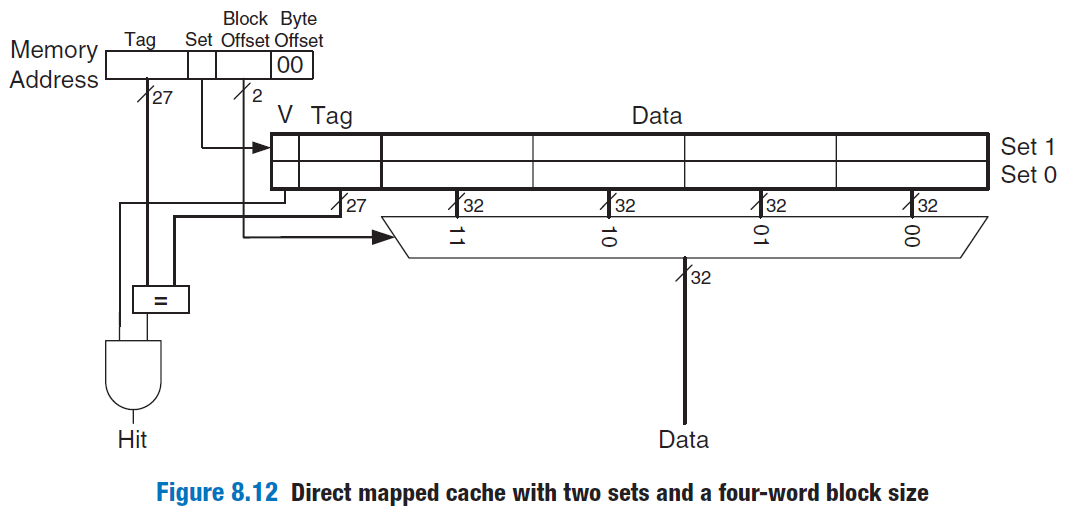
\includegraphics[width=0.55\textwidth]{figures/fig8.12.png}
    \caption{Direct mapped cache with two sets and a 4-word block size (Harris Figure~8.12). The block offset bits [$3$:$2$] control a 4:1 multiplexer to select the word within the block. Only 1 set bit is needed ($\log_2 2 = 1$).}
    \label{fig:cache-blk-hw}
\end{figure}

The address field decomposition for this cache:

\begin{center}
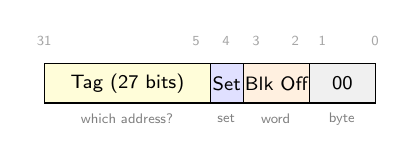
\begin{tikzpicture}[
  every node/.style={transform shape},
  fld/.style={draw, minimum height=0.5cm, inner sep=0pt,
              font=\sffamily\scriptsize, text centered},
  bit/.style={font=\sffamily\tiny\color{gray!70}, anchor=south}]

  \def\bp{0.42}

  % Field widths: Tag[31:5]=5bp, Set[4]=1bp, BlkOff[3:2]=2bp, Byte[1:0]=2bp → total 10bp
  % Boundaries at x = 0, 5bp, 6bp, 8bp, 10bp

  % Bit labels at field boundaries
  \node[bit] at (0, 0.35) {31};
  \node[bit, anchor=south east] at (5*\bp, 0.35) {5};
  \node[bit] at (5.5*\bp, 0.35) {4};
  \node[bit, anchor=south west] at (6*\bp, 0.35) {3};
  \node[bit, anchor=south east] at (8*\bp, 0.35) {2};
  \node[bit, anchor=south west] at (8*\bp, 0.35) {1};
  \node[bit] at (10*\bp, 0.35) {0};

  % Fields
  \node[fld, fill=yellow!15, minimum width=5*\bp cm, anchor=west] at (0, 0) {Tag (27 bits)};
  \node[fld, fill=blue!12, minimum width=1*\bp cm, anchor=west] at (5*\bp, 0) {Set};
  \node[fld, fill=orange!12, minimum width=2*\bp cm, anchor=west] at (6*\bp, 0) {Blk Off};
  \node[fld, fill=gray!12, minimum width=2*\bp cm, anchor=west] at (8*\bp, 0) {00};

  % Labels below (centered under each field)
  \node[font=\sffamily\tiny, text=gray] at (2.5*\bp, -0.45) {which address?};
  \node[font=\sffamily\tiny, text=gray] at (5.5*\bp, -0.45) {set};
  \node[font=\sffamily\tiny, text=gray] at (7*\bp, -0.45) {word};
  \node[font=\sffamily\tiny, text=gray] at (9*\bp, -0.45) {byte};

\end{tikzpicture}
\end{center}

\paragraph{Example: spatial locality (Harris 8.9).} Repeating the loop from Example~8.6 with a 4-word block: the first access to address 0x4 misses and loads addresses 0x0--0xC into one cache block. All 14 subsequent accesses (to 0x4, 0xC, 0x8) hit. Miss rate drops from 20\% to $1/15 = 6.67\%$.

The trade-off: larger block sizes reduce compulsory misses (spatial locality) but decrease the number of sets in a fixed-size cache, which can increase conflicts. Larger blocks also increase the \textbf{miss penalty} --- the time to fetch a multi-word block from main memory. For most programs, blocks of 32--64 bytes strike a good balance.

\paragraph{Summary.} Table~\ref{tab:cache-org} summarises the three cache organisations. In general, the address is decomposed as:

$$
\underbrace{\text{Tag}}_{\text{remaining MSBs}} \;\Big|\; \underbrace{\text{Set}}_{\log_2 S \text{ bits}} \;\Big|\; \underbrace{\text{Block Offset}}_{\log_2 b \text{ bits}} \;\Big|\; \underbrace{\text{Byte Offset}}_{\log_2 4 = 2 \text{ bits}}
$$

Increasing associativity $N$ reduces conflict misses but requires more comparators. Increasing block size $b$ exploits spatial locality but may increase conflicts and miss penalty.

\begin{table}[htbp]
\centering\small
\begin{tabular}{@{}l c c@{}}
    \toprule
    Organisation & Ways ($N$) & Sets ($S$) \\
    \midrule
    Direct Mapped & 1 & $B$ \\
    $N$-way Set Associative & $1 < N < B$ & $B/N$ \\
    Fully Associative & $B$ & 1 \\
    \bottomrule
\end{tabular}
\caption{Cache organisations (Harris Table~8.2). Each address maps to exactly one set but can be stored in any of the $N$ ways.}
\label{tab:cache-org}
\end{table}

\subsubsection{What Data is Replaced?}

In a direct mapped cache, each address maps to a unique block, so replacement is trivial: the old block is evicted. In set associative and fully associative caches, when all ways in a set are full, the cache must choose which block to evict. The principle of temporal locality suggests evicting the \textbf{least recently used} (LRU) block, since it is least likely to be needed again soon.

In a 2-way set associative cache, a single \textbf{use bit} $U$ tracks which way was least recently used: each time one way is accessed, $U$ is set to indicate the \emph{other} way. On replacement, the block in the way indicated by $U$ is evicted.

For higher associativity ($N > 2$), exact LRU tracking becomes expensive ($\log_2(N!)$ bits per set). In practice, \textbf{pseudo-LRU} is used: the ways are divided into two groups, $U$ indicates which group was least recently used, and replacement picks a random block from that group.

\subsubsection{Advanced Cache Design}

\paragraph{Multi-level caches.} Modern systems use at least two cache levels. The \textbf{L1 cache} is small and fast (1--2 cycle access); the \textbf{L2 cache} is larger but slower ($\sim$10 cycles). The processor checks L1 first; on an L1 miss, it checks L2; on an L2 miss, it goes to main memory.

\paragraph{Reducing miss rate.} Cache misses are classified into three types:

\begin{itemize}
    \item \textbf{Compulsory} (cold-start): the first access to a block always misses, regardless of cache design. Larger block sizes reduce compulsory misses (spatial locality).
    \item \textbf{Capacity}: the cache is too small to hold all concurrently needed data. Increasing cache size reduces capacity misses.
    \item \textbf{Conflict}: multiple addresses map to the same set and evict blocks that are still needed. Increasing associativity reduces conflict misses, but beyond 4--8 ways the improvement is small.
\end{itemize}

Increasing block size reduces compulsory misses but may \emph{increase} conflict misses (fewer sets in a fixed-size cache). For small caches ($\leq$4\,KiB), block sizes beyond 64 bytes increase overall miss rate; for larger caches the effect is less pronounced.

\paragraph{Write policy.} When the processor stores data to an address that is in the cache, the cache block is updated. The question is whether main memory is also updated:

\begin{itemize}
    \item \textbf{Write-through}: every store simultaneously writes to both the cache and main memory. Simple, but generates many slow main memory writes.
    \item \textbf{Write-back}: the cache block is marked with a \textbf{dirty bit} $D$. $D = 1$ means the block has been modified since it was loaded. Dirty blocks are written back to main memory only when \emph{evicted} from the cache. This is far more efficient: if a block is written $k$ times before eviction, write-back saves $k - 1$ main memory writes.
\end{itemize}

Modern caches universally use write-back because the main memory access time ($\sim$100 cycles) makes write-through impractical. On a store that misses in the cache, the block is first fetched from main memory into the cache (\textbf{write-allocate}), then the store is applied to the cache copy.\footnote{\textbf{Virtual memory} (Harris~\S8.4) extends the memory hierarchy to disk: programs use virtual addresses translated to physical addresses via page tables, with a TLB (fully associative cache of page table entries) eliminating the double-access penalty for $>$99\% of accesses. Virtual memory also provides memory protection (per-process page tables). The picorv32 on the iCE40UP5K has no MMU --- all addresses are physical --- so virtual memory does not apply to this project.}

\newpage
\section{Hardware: iCE40UP5K}

\begin{comment}
Since I have close to zero knowledge of FPGA architecture, this section covers the fundamental core ideas of this FPGA architecture, borrowing concepts from the books above and datasheets

The github repo with core hardware details is 
- 'https://github.com/icebreaker-fpga/icebreaker/tree/master' definitely read the README file
- specifically the 1.1a variant 'https://github.com/icebreaker-fpga/icebreaker/tree/master/hardware/v1.1a'
\end{comment}

The iCEBreaker board carries a Lattice \textbf{iCE40UP5K} FPGA chip. The board also contains (outside chip) contain a 12\,MHz clock, 128\,Mbit QSPI flash (W25Q128JV) for bitstream and firmware storage, and an FT2232H for USB programming and UART.

\subsection{Resource budget}

Table~\ref{tab:resources} lists the on-chip resources. For the later picorv32 RISC-V implementation, the binding constraints are logic cells (the CPU datapath and control) and memory (instruction/data storage in EBR and SPRAM).

\begin{table}[htbp]
\centering\small
\begin{tabular}{@{}l r l@{}}
    \toprule
    Resource & Count & Notes \\
    \midrule
    Logic Cells (4-LUT + FF) & 5280 & 660 PLBs $\times$ 8 LCs; each LC has carry logic \\
    EBR (4\,Kb dual-port RAM) & 30 & 120\,Kb (15KB) total; configurable as 256$\times$16 to 2048$\times$2 \\
    SPRAM (256\,Kb single-port) & 4 & 1024\,Kb (128KB) total; 16K$\times$16 fixed width, not pre-loadable \\
    DSP (16$\times$16 MAC) & 8 & $\geq$50\,MHz; can split into two 8$\times$8 multipliers \\
    PLL & 1 & output divider $2^0$--$2^6$; HFOSC 48\,MHz / LFOSC 10\,kHz also available \\
    I/O pins & 39 & 3 banks: Bank\,0 (17), Bank\,1 (14), Bank\,2 (8) \\
    \bottomrule
\end{tabular}
\caption{iCE40UP5K-SG48 resource summary.}
\label{tab:resources}
\end{table}

Figure~\ref{fig:ice40-top} shows the top-level floorplan. The PLB rows occupy the centre, flanked by columns of EBR (labelled ``4\,Kb DPRAM'') and DSP blocks. The four SPRAM blocks sit along the bottom edge. I/O banks surround the perimeter, with the clock (PLL, HFOSC, LFOSC) along the top.

\begin{figure}[htbp]
    \centering
    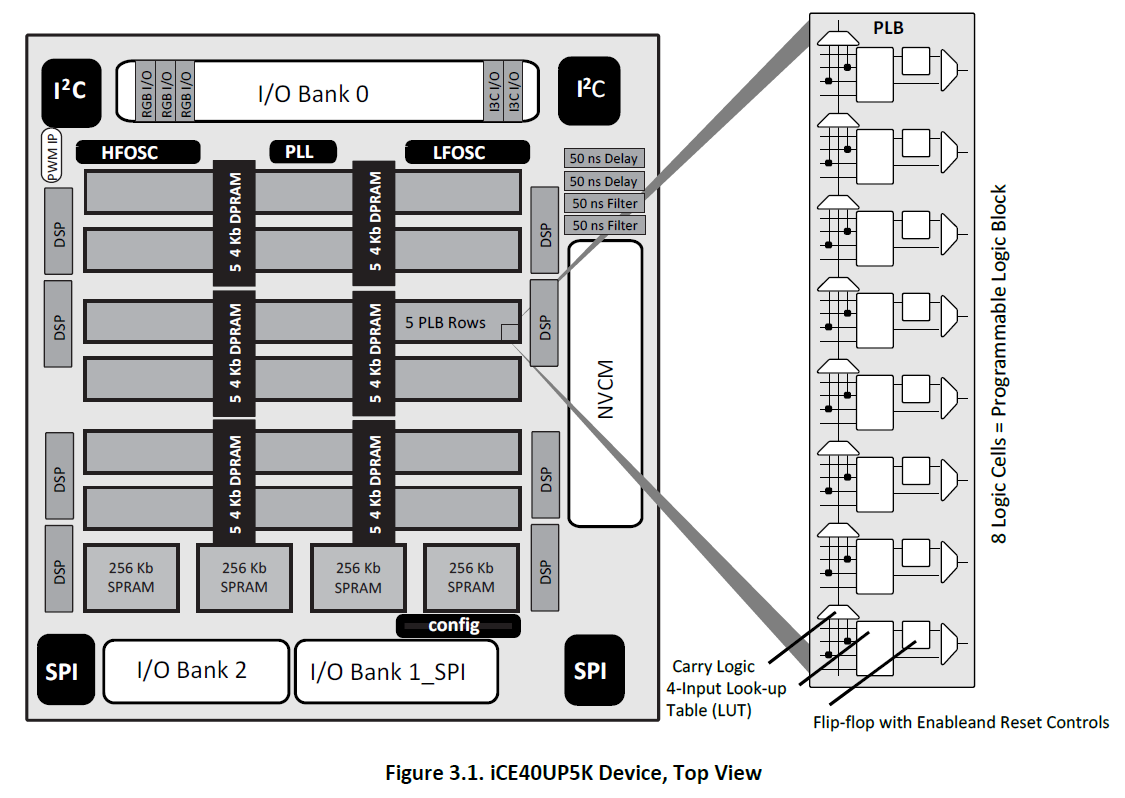
\includegraphics[width=0.85\textwidth]{figures/fig3.1.png}
    \caption{iCE40UP5K device floorplan (datasheet Fig.\ 3.1). The inset shows a single PLB: 8 Logic Cells, each containing a 4-input LUT, carry logic, and a flip-flop.}
    \label{fig:ice40-top}
\end{figure}

\subsection{Logic Cells and Programmable Logic Blocks}

\begin{comment}
READ: Harris §5.6.2 (FPGA), specifically the LUT-based logic cell explanation
READ: Harris §5.5.7 (Logic Using Memory Arrays) --- LUT = SRAM truth table
READ: Datasheet §3.1.1 (PLB Blocks), Figure 3.2
\end{comment}

Each \textbf{Logic Cell (LC)} pairs one 4-LUT with one D flip-flop and dedicated carry logic:

\begin{itemize}
    \item \textbf{4-LUT}: computes any combinational function of up to 4 inputs. For wider functions (e.g.\ a 7-input XOR), multiple LUTs are cascaded.
    \item \textbf{D flip-flop}: stores one bit of state, clocked with optional enable and synchronous set/reset. A multiplexer at the output selects between the LUT result (combinational path) and the FF output (registered path).
    \item \textbf{Carry chain}: a dedicated fast-ripple path (FCIN $\to$ carry logic $\to$ FCOUT) that bypasses the general routing. This lets adders and counters use just one LC per bit --- the LUT computes the sum/generate/propagate, and the carry chain handles the carry, without consuming extra LUTs.
\end{itemize}

Figure~\ref{fig:plb} shows the detailed structure. Within each LC, the LUT output and the carry logic feed a multiplexer whose output can go directly to the output pin O (combinational) or through the DFF (registered). The carry chain (FCIN/FCOUT) threads vertically through all 8 LCs in the PLB, enabling fast arithmetic without using the general routing fabric.

\begin{figure}[htbp]
    \centering
    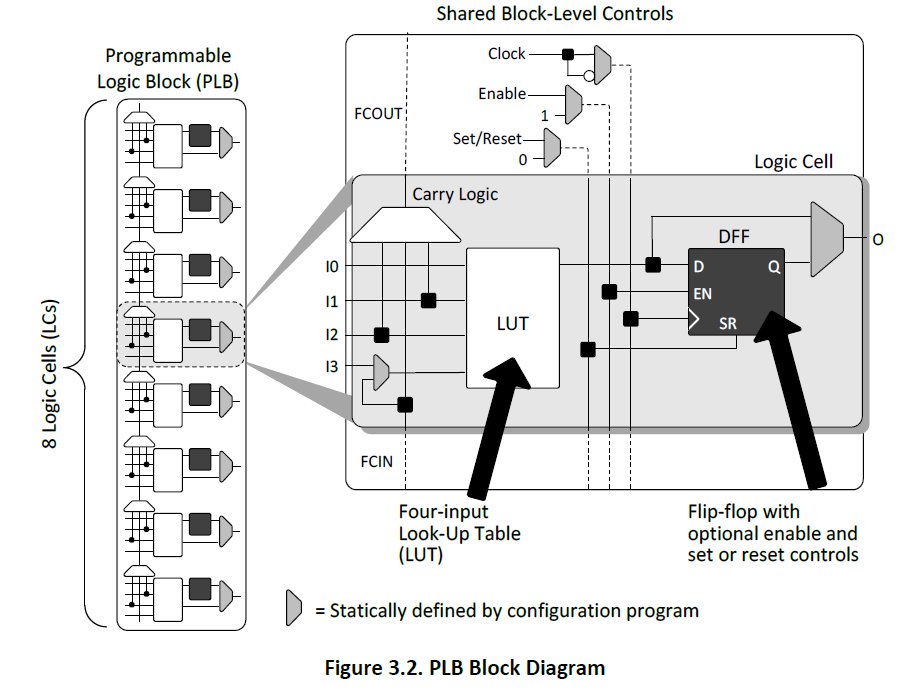
\includegraphics[width=0.75\textwidth]{figures/fig3.2.png}
    \caption{PLB block diagram (datasheet Fig.\ 3.2). Left: 8 LCs in a column with shared block-level controls (clock, enable, set/reset). Right: detail of one LC showing the 4-input LUT, carry logic, and D flip-flop.}
    \label{fig:plb}
\end{figure}

Eight LCs are grouped into one \textbf{Programmable Logic Block (PLB)}, sharing a common clock, clock-enable, and set/reset signal. The shared controls reduce routing overhead --- all eight FFs in a PLB are clocked together.

\subsection{EBR/DPRAM}

\begin{comment}
READ: Harris §5.5 (Memory Arrays), specifically §5.5.1--5.5.5
READ: Datasheet §3.1.5 (sysMEM EBR), Figure 3.4, Table 3.4
\end{comment}

The Embedded Block RAM (EBR) blocks are the FPGA's fast, \textit{dual-port} on-chip memory (Dual Port Memory or DPRAM). Each block holds 4\,Kbit with a \textit{maximum data-port width of 16 bits}, and can be configured in several aspect ratios:

\begin{table}[htbp]
\centering\small
\begin{tabular}{@{}l l l@{}}
    \toprule
    Configuration & Depth $\times$ Width & Address bits \\
    \midrule
    256$\times$16 & 256 words, 16-bit & 8 \\
    512$\times$8  & 512 words, 8-bit  & 9 \\
    1024$\times$4 & 1024 words, 4-bit & 10 \\
    2048$\times$2 & 2048 words, 2-bit & 11 \\
    \bottomrule
\end{tabular}
\caption{EBR block configurations (each 4\,Kbit).}
\label{tab:ebr-config}
\end{table}

\begin{itemize}
    \item \textbf{Dual-port (1R1W)}: one read port and one write port, each with its own address, clock, and enable. A reader and a writer can therefore access the block in the same cycle (e.g.\ the register file reads \texttt{rs1} while the previous instruction writes \texttt{rd}).
    \item \textbf{Pre-loadable}: contents can be initialised during FPGA configuration (the values are embedded in the bitstream), making EBR usable as ROM or pre-filled RAM. \footnote{However iCEon the iCEBreaker the program lives in SPI flash and is fetched at runtime via \texttt{spimemio} (reset vector at \texttt{0x00100000}, \S\ref{sec:picosoc}). EBR pre-loading is how a BRAM-backed instruction memory \emph{would} work (and how the generic \texttt{picosoc\_mem} variant loads code), but it is not how this board boots.}
    \item \textbf{Fast}: operates up to 150\,MHz register-to-register.
    \item \textbf{Cascadable}: multiple blocks can be used together for wider or deeper memories. Because the data port is at most 16 bits wide, building a 32-bit width memory must pair two blocks side-by-side (one for bits \texttt{[15:0]}, one for \texttt{[31:16]}).
\end{itemize}

\subsection{SPRAM}

\textit{Single Port Memory} SPRAM provides bulk storage: four 256\,Kbit blocks totalling 1\,Mbit (128\,KB). Unlike EBR, each SPRAM block is fixed at 16K words $\times$ 16 bits with a single read/write port.

\begin{itemize}
    \item \textbf{Single-port}: a given block can either read or write in any clock cycle, never both simultaneously. To build a 32-bit data memory, two SPRAM blocks are used side-by-side (one for the upper 16 bits, one for the lower 16 bits), but both share the same address.
    \item \textbf{Not pre-loadable}: SPRAM contents are undefined after configuration. Firmware must initialise it at runtime.
    \item \textbf{Nibble write masking}: the 4-bit MASKWREN signal allows writing individual nibbles (4-bit groups) within the 16-bit word, enabling byte-granularity stores.
    \item \textbf{Slower}: maximum 70\,MHz, compared to EBR's 150\,MHz
    \item \textbf{Power}: Supports Standby/Sleep/Power Off modes for reducing power when idle.
\end{itemize}

% TODO: screenshot of datasheet Figure 3.5 (SPRAM Primitive)
% shows ADDRESS[13:0], DATAIN[15:0], DATAOUT[15:0], MASKWREN[3:0], WREN, CHIPSELECT, CLOCK

\subsection{DSP Blocks}

\begin{comment}
READ: Harris §5.2.6 (Multiplication --- shift-and-add vs hardware multiplier)
READ: Datasheet §3.1.7 (sysDSP), Figures 3.6--3.8, Tables 3.7, §4.20 (DSP Timing)
\end{comment}

The 8 sysDSP blocks are hardened \textbf{multiply-accumulate (MAC)} units in dedicated silicon, running at 50\,MHz with no LUT cost --- implementing the same 16$\times$16 multiply in LUTs would consume hundreds of logic cells. The picorv32 uses four DSP blocks for \texttt{pcpi\_fast\_mul} (a signed 32$\times$32 multiply built from four 16$\times$16 MACs; Section~\ref{sec:pcpi}), leaving four free.

\subsubsection{MAC datapath}

Each DSP block performs the \textbf{multiply-accumulate (MAC)} operation: $\text{acc} \leftarrow \text{acc} + a \cdot b$. This is the inner loop of matrix multiplication. To compute one output element $C_{ij}$, the MAC computes the dot product of row $\mathbf{a} = A[i,:]$ and column $\mathbf{b} = B[:,j]$, streaming one element pair per cycle:

\noindent
\begin{minipage}[t]{0.40\textwidth}
\vspace{0pt}
$$
\begin{aligned}
C_{ij} &= \sum_{k=0}^{N-1} A_{ik}\, B_{kj} \\[4pt]
       &= \mathbf{a} \cdot \mathbf{b} = \sum_{k=0}^{N-1} a_k \, b_k
\end{aligned}
$$
\vspace{-6pt}
\centering\footnotesize
where $\mathbf{a} = A[i,:]$,\; $\mathbf{b} = B[:,j]$
\end{minipage}%
\hfill
\begin{minipage}[t]{0.4\textwidth}
\vspace{0pt}
\begin{algorithm}[H]
\footnotesize
\caption{MAC (one DSP, $N$ cycles)}
\begin{algorithmic}[1]
\State $\text{acc} \gets 0$ \Comment{preload via C/D}
\For{$k = 0$ \textbf{to} $N-1$} \Comment{1 cycle each}
    \State $\text{acc} \gets \text{acc} + a_k \cdot b_k$
\EndFor
\State $C_{ij} \gets \text{acc}$
\end{algorithmic}
\end{algorithm}
\end{minipage}

\vspace{6pt}

For 16-bit integers $a_k$ and $b_k$, Figure~\ref{fig:dsp-datapath} shows the hardware datapath.

\begin{figure}[htbp]
    \centering
    \begin{minipage}[b]{0.68\textwidth}
    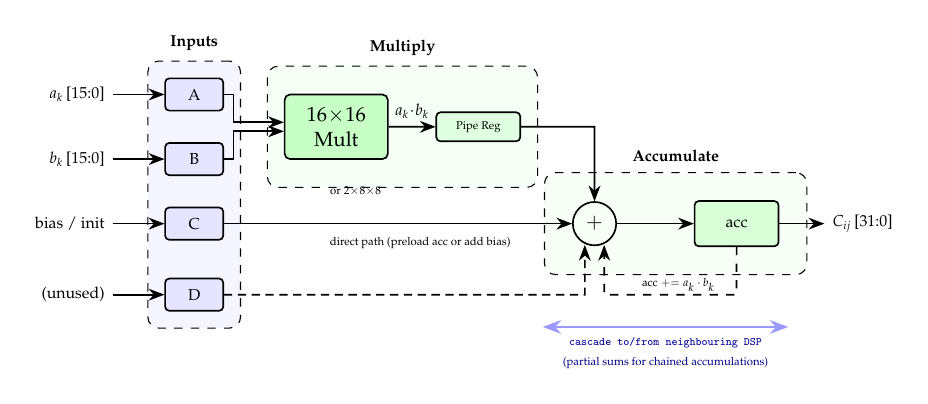
\begin{tikzpicture}[>=Stealth, semithick, scale=0.82, every node/.style={transform shape},
      reg/.style={draw, fill=blue!10, minimum width=0.9cm, minimum height=0.5cm,
                  font=\scriptsize, rounded corners=1.5pt},
      blk/.style={draw, fill=green!22, minimum width=1.6cm, minimum height=1.0cm,
                  font=\small, align=center, rounded corners=2pt},
      pipreg/.style={draw, fill=green!12, minimum width=1.3cm, minimum height=0.45cm,
                  font=\tiny, rounded corners=1.5pt},
      pm/.style={draw, circle, minimum size=0.65cm, font=\small},
      acc/.style={draw, fill=green!15, minimum width=1.3cm, minimum height=0.7cm,
                  font=\scriptsize, rounded corners=1.5pt},
      stage/.style={draw, dashed, rounded corners=4pt, inner sep=6pt},
      lbl/.style={font=\scriptsize},
      casc/.style={font=\tiny\ttfamily, text=blue!60!black}]

    % ---- Top path: A,B -> multiply ----
    \node[reg] (rA) at (0, 1.8) {A};
    \node[reg] (rB) at (0, 0.8) {B};
    \node[blk] (mult) at (2.2, 1.3) {$16\!\times\!16$\\Mult};
    \node[pipreg] (pip) at (4.4, 1.3) {Pipe Reg};

    \draw[<-] (rA.west) -- ++(-0.8,0) node[left,lbl] {$a_k$\,[15:0]};
    \draw[<-] (rB.west) -- ++(-0.8,0) node[left,lbl] {$b_k$\,[15:0]};
    \draw[->] (rA.east) -- ++(0.15,0) |- ([yshift=2pt]mult.west);
    \draw[->] (rB.east) -- ++(0.15,0) |- ([yshift=-2pt]mult.west);
    \draw[->] (mult) -- (pip) node[midway, above, lbl] {$a_k \!\cdot\! b_k$};

    % ---- Middle: adder + accumulator ----
    \node[pm] (pm) at (6.2, -0.2) {$+$};
    \node[acc] (acc) at (8.4, -0.2) {acc};

    % Product: pipe reg -> right -> down to + (enters from north)
    \draw[->] (pip.east) -- (6.2, 1.3) -- (pm.north);
    \draw[->] (pm) -- (acc);
    \draw[->] (acc.east) -- ++(0.7,0) node[right,lbl] {$C_{ij}$\,[31:0]};

    % ---- Bottom path: C,D bypass (preload) ----
    \node[reg] (rC) at (0, -0.2) {C};
    \node[reg] (rD) at (0, -1.3) {D};
    \draw[<-] (rC.west) -- ++(-0.8,0) node[left,lbl] {bias / init};
    \draw[<-] (rD.west) -- ++(-0.8,0) node[left,lbl] {(unused)};

    \draw[->] (rC.east) -- (pm.west);
    % D: right to x=5.9 at y=-1.3, then straight up into pm (left of centre)
    \draw[->, densely dashed] (rD.east) -- (6.05,-1.3) -- (6.05,-0.53);
    \node[font=\tiny] at (3.5,-0.5) {direct path (preload acc or add bias)};
    \node[font=\tiny] at (2.5, 0.3) {or $2\!\times\!8\!\times\!8$};

    % Feedback: acc south down to y=-1.3 (same level as D horizontal), then left to x=6.35, then up into pm (right of centre)
    \draw[->, dashed] (acc.south) -- (8.4,-1.3) -- (6.35,-1.3) -- (6.35,-0.53);
    \node[font=\tiny] at (7.5,-1.15) {$\text{acc} \mathrel{+}= a_k \cdot b_k$};

    % ---- Cascade signals ----
    \draw[<->, blue!40, thick] (5.4,-1.8) -- (9.2,-1.8);
    \node[casc, align=center] at (7.3,-2.05) {cascade to/from neighbouring DSP};
    \node[font=\tiny, text=blue!50!black] at (7.3,-2.35) {(partial sums for chained accumulations)};

    % ---- Stage outlines ----
    \begin{scope}[on background layer]
    \node[stage, fill=blue!4, fit=(rA)(rB)(rC)(rD),
          label={[font=\scriptsize\bfseries, yshift=1pt]above:Inputs}] {};
    \node[stage, fill=green!4, fit=(mult)(pip), inner ysep=10pt,
          label={[font=\scriptsize\bfseries, yshift=1pt]above:Multiply}] {};
    \node[stage, fill=green!3, fit=(pm)(acc), inner sep=10pt,
          label={[font=\scriptsize\bfseries, yshift=1pt]above:Accumulate}] {};
    \end{scope}

    \end{tikzpicture}
    \end{minipage}%
    \hfill
    \begin{minipage}[b]{0.28\textwidth}
    \centering
    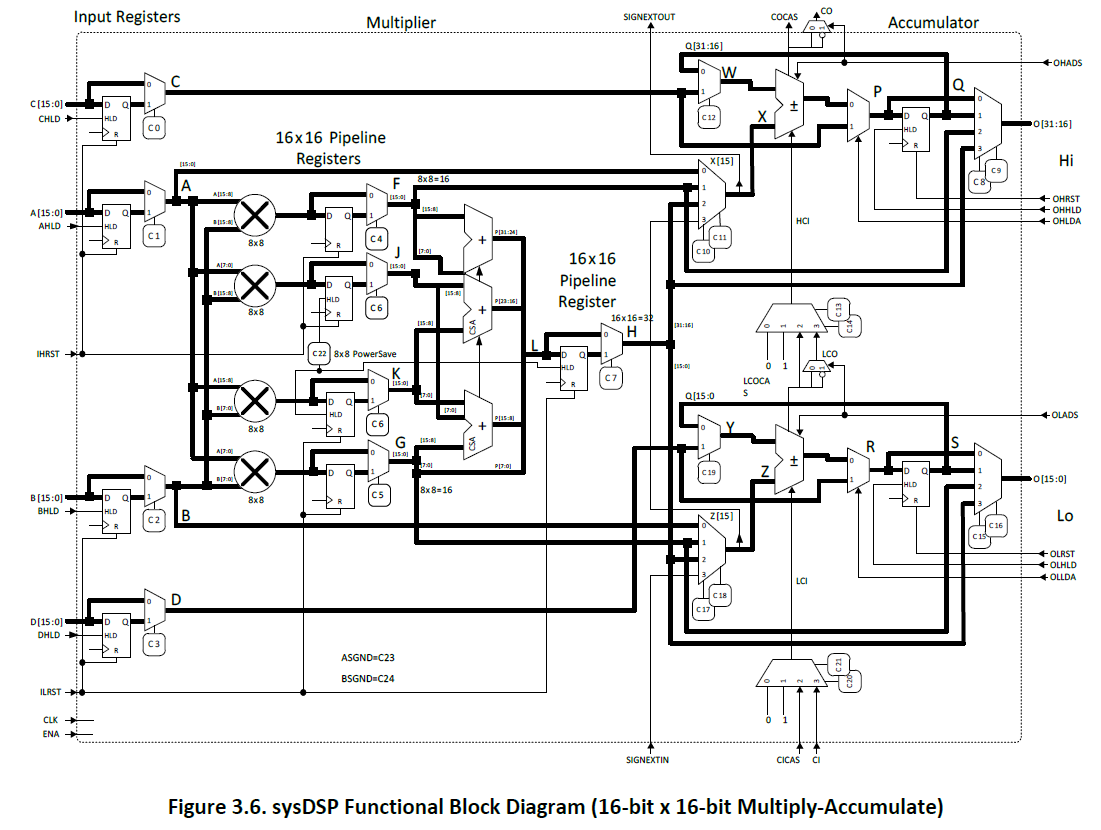
\includegraphics[width=\textwidth]{figures/fig3.6.png}
    \vspace{2pt}
    {\footnotesize Datasheet Fig.\ 3.6}
    \end{minipage}
    \caption{Left: simplified sysDSP datapath. Inputs $a_k$, $b_k$ stream through the multiplier; the accumulator feedback (dashed) adds each product to a running sum. C/D bypass the multiplier to preload the accumulator. Cascade signals connect to neighbouring DSPs for chained operations. Right: full datasheet block diagram showing dual 8$\times$8 mode paths.}
    \label{fig:dsp-datapath}
\end{figure}

The multiplier operates in two modes: one 16$\times$16 $\to$ 32-bit product, or two independent 8$\times$8 $\to$ 16-bit products (for int8 inference). An optional pipeline register between multiplier and accumulator breaks the critical path for higher clock rates at the cost of one cycle latency.

\subsubsection{Cascading}

Adjacent DSP blocks have dedicated cascade signals (\textbf{SIGNEXTIN/SIGNEXTOUT} for sign-extension chains, \textbf{CICAS/COCAS} for carry/borrow) that enable wider multiplications or chained accumulations through hardened wiring rather than the general routing fabric. Maximum clock: 50\,MHz (with pipeline register bypassed).

\subsection{Clocking}

The board provides a 12\,MHz crystal oscillator. The on-chip PLL synthesises higher frequencies using three divider parameters:

$$
f_{\text{out}} = f_{\text{ref}} \times \frac{\texttt{DIVF} + 1}{(\texttt{DIVR} + 1) \times 2^{\texttt{DIVQ}}}
$$

where $f_{\text{ref}} = 12$\,MHz, \texttt{DIVR} is the reference divider (0--15), \texttt{DIVF} is the feedback divider (0--63), and \texttt{DIVQ} is the output divider (1--6). The VCO frequency must stay within 533--1066\,MHz; \texttt{DIVQ} then divides the VCO output down to the desired clock. Practically, the Lattice \texttt{icepll} tool computes valid settings: \texttt{icepll -i 12 -o 24} produces a configuration for 24\,MHz.

The maximum frequency for the global clock network is 185\,MHz (Table~4.21 of the datasheet). The binding constraints on the system clock for PicoSoC are:

\begin{center}\small
\begin{tabular}{@{}l r l@{}}
    \toprule
    Resource & Max freq & Constraint \\
    \midrule
    Global clock buffer & 185\,MHz & routing fabric limit \\
    SPRAM & 70\,MHz & data memory access \\
    DSP (bypassing pipeline reg) & 50\,MHz & \texttt{pcpi\_fast\_mul} \\
    EBR & 150\,MHz & instruction cache (if added) \\
    \bottomrule
\end{tabular}
\end{center}

The system clock must not exceed the slowest component on the critical path. With SPRAM at 70\,MHz and DSP at 50\,MHz, the practical ceiling is $\sim$48\,MHz (allowing margin for routing delay and timing closure). The baseline iCEBreaker design runs at 12\,MHz (no PLL); adding a PLL to run at 24\,MHz would roughly double throughput with no other changes.

\paragraph{System clock vs.\ peripheral clocks.} The system clock is the single clock that drives the CPU core, EBR, SPRAM, and all on-chip logic. However, external peripherals have their own clocks that are \emph{derived from} the system clock but run at different rates. The most important example is the \textbf{SPI flash clock} (SCK): \texttt{spimemio} generates the SPI serial clock by dividing the system clock, typically by 2 (so 6\,MHz SCK at 12\,MHz system). Every SPI transaction is measured in \emph{SPI clocks} --- e.g.\ a QSPI read costs $\sim$22 SPI clocks --- but the CPU stalls for the corresponding number of \emph{system cycles}, which is $22 \times (f_{\text{sys}} / f_{\text{SPI}})$ system cycles. At a 2:1 ratio, 22 SPI clocks = 44 system cycles during which the CPU cannot fetch the next instruction. Raising the system clock with a PLL (with the divider locked at 2:1) raises SCK in lockstep, so a fetch still costs the same \emph{number of system cycles} --- only the wall-clock time shrinks with $f_{\text{sys}}$. Cutting the system-cycle cost itself requires either fewer SPI clocks per word (fast-read modes, Section~\ref{sec:fastflash}) or a tighter divider ratio. SPRAM and EBR, by contrast, are synchronous to the system clock and respond in 1 system cycle --- no clock-domain crossing.

\begin{comment}
TODO: After synthesis, check the actual fmax reported by nextpnr (nextpnr --up5k ... reports
"Max frequency for clock 'clk': XX.XX MHz"). This determines the real ceiling.
Use: icepll -i 12 -o <target> to compute PLL parameters.
\end{comment}

\subsection{Power Characteristics}

Dynamic power scales linearly with frequency, switching activity, and capacitance ($P_{\text{dyn}} = \alpha C V^2 f$). Static (leakage) power is fixed by the process. The iCE40UP5K datasheet specifies:

\begin{center}\small
\begin{tabular}{@{}l r@{}}
    \toprule
    Parameter & Typical \\
    \midrule
    Core standby current ($V_{\text{CC}}$=1.2\,V, 0\,MHz) & 75\,$\mu$A \\
    Core startup peak current & 12\,mA \\
    SPRAM standby current & 0.55\,$\mu$A \\
    \bottomrule
\end{tabular}
\end{center}

Adding logic (cache controller, pipeline registers, hazard unit) increases both switching activity and capacitive load, raising dynamic power. Enabling the PLL itself draws additional current. However, if the higher clock frequency reduces execution time, the \emph{total energy} per benchmark ($E = P \times t$) may decrease even though instantaneous power rises --- the processor finishes sooner and returns to idle.

\begin{comment}
TODO: Measure power for three configurations using the lab multimeter:
  1. Inverter baseline (inv_baseline.v) — reference for static power
  2. Baseline PicoSoC running blink.c at 12 MHz — dynamic power baseline
  3. Optimised PicoSoC (cache + pipeline) at 24 MHz — compare energy per iteration
Record: supply voltage, supply current, computed power. Use Picoscope to measure
execution time per iteration for energy calculation.
\end{comment}

\subsection{Board-Level Connectivity}

\begin{comment}
READ: iCEBreaker schematic (icebreaker-sch.pdf), iCEBreaker GitHub README
READ: Datasheet §5.1--5.2 (Pinout)
\end{comment}

The iCEBreaker board connects the iCE40UP5K to the rest of the peripherals on board:

\begin{itemize}
    \item \textbf{FT2232H}: USB-to-FPGA bridge providing both JTAG programming (iceprog) and a UART channel (115200 baud). Channel A programs the FPGA; channel B provides serial I/O for the PicoSoC console.
    \item \textbf{12\,MHz crystal oscillator}: reference clock for the PLL, shared with the FT2232H.
    \item \textbf{W25Q128JV flash} (128\,Mbit): stores the FPGA bitstream and (in PicoSoC) firmware, accessed via QSPI.
    \item \textbf{PMOD headers}: dual PMOD (16 pins) and single PMOD (8 pins). PMOD1A is mapped to a 7-segment display in the modified PicoSoC.
    \item \textbf{LEDs and buttons}: 2 on-board LEDs, 1 push button, plus 5 LEDs and 3 buttons on the snap-off section.
\end{itemize}

\newpage

\section{picorv32 Microarchitecture}

We implement the \texttt{picorv32} micoarchitecture on the \texttt{icebreaker} chip. Figure~\ref{fig:hierarchy-tree} shows how the Verilog modules connect: \texttt{icebreaker} (top-level board) instantiates \texttt{picosoc} system-on-chip plus the board-specific components --- four \texttt{flash\_io\_buf} \texttt{SB\_IO} buffers (the QSPI flash pins) and \texttt{seven\_seg\_ctrl} (which contains \texttt{seven\_seg\_hex}). \texttt{picosoc} contains the \texttt{picorv32} CPU core, \texttt{spimemio} (which contains \texttt{spimemio\_xfer}, the SPI shift engine), \texttt{simpleuart}, and \texttt{ice40up5k\_spram} (four \texttt{SB\_SPRAM256KA} SPRAM blocks). The CPU itself contains \texttt{picosoc\_regs} (register file) and \texttt{picorv32\_pcpi\_fast\_mul} (hardware multiplier mapping to DSP blocks).

\begin{figure}[htbp]
    \centering
    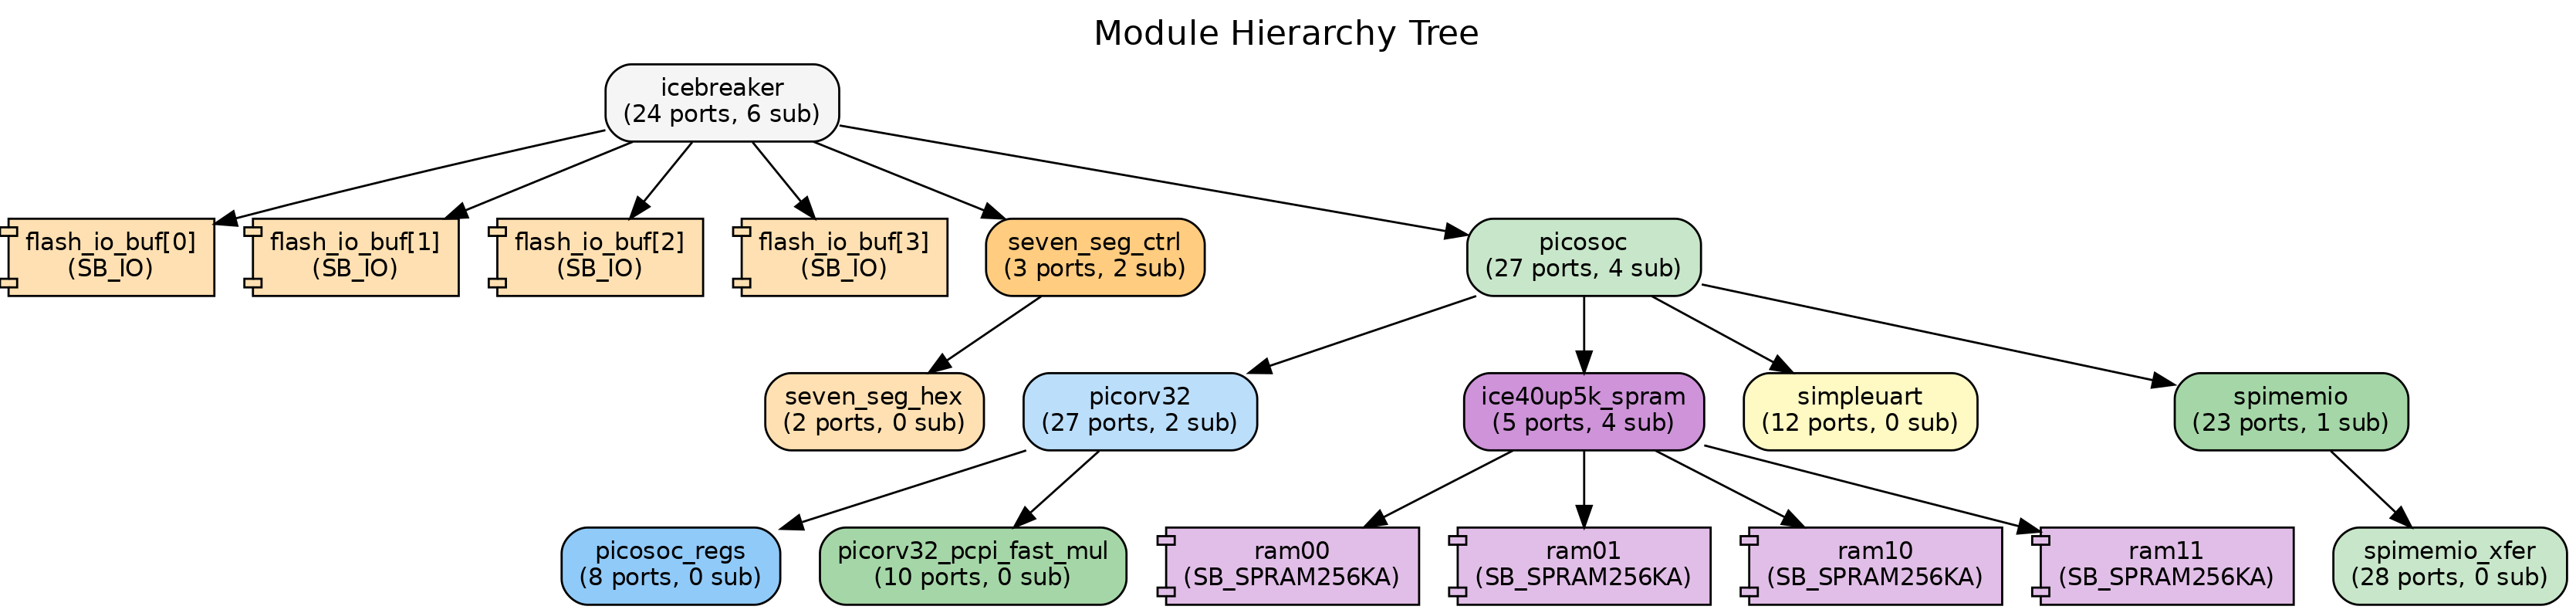
\includegraphics[width=\textwidth]{figures/arch/10_hierarchy_tree.png}
    \caption{Module hierarchy tree (auto-extracted from yosys elaboration). Each node shows the module name, port count, and number of submodule instances. Leaf nodes with \texttt{SB\_*} types are iCE40 hard IP primitives.}
    \label{fig:hierarchy-tree}
\end{figure}

The picorv32 is highly configurable via Verilog \texttt{parameter} declarations. Each parameter trades LUT area against cycle count or critical path length. Table~\ref{tab:picorv32-params} lists the key knobs with their iCEBreaker defaults (from \texttt{icebreaker.v}) and trade-off notes.

\begin{table}[htbp]
\centering\scriptsize
\renewcommand{\arraystretch}{1.25}
\begin{tabular}{@{}l c c p{7.5cm}@{}}
    \toprule
    Parameter & Default & iCEBreaker & Trade-off \\
    \midrule
    \texttt{BARREL\_SHIFTER} & 0 & 0 &
        \textbf{0}: shifts iterate 1--4 bits/cycle in \texttt{shift} state ($3{+}N$ cycles). \textbf{1}: combinational barrel shifter in ALU (3 cycles, $\sim$200 extra LUTs). \\
    \texttt{TWO\_STAGE\_SHIFT} & 1 & 1 &
        When \texttt{BARREL\_SHIFTER}=0: \textbf{1}: shifts 4 bits/cycle when $\texttt{reg\_sh} \geq 4$, then 1 bit/cycle. \textbf{0}: always 1 bit/cycle (up to 31 cycles). \\
    \texttt{TWO\_CYCLE\_ALU} & 0 & 0 &
        \textbf{0}: ALU is combinational (\texttt{always @*}). \textbf{1}: ALU is registered (\texttt{always @(posedge clk)}), adds 1 cycle latency but shortens critical path. \\
    \texttt{TWO\_CYCLE\_COMPARE} & 0 & 0 &
        \textbf{1}: branch comparisons take an extra cycle (registers the comparator output). Reduces critical path for branch instructions. \\
    \texttt{ENABLE\_REGS\_DUALPORT} & 1 & 1 &
        \textbf{1}: register file has two read ports; both \texttt{rs1} and \texttt{rs2} read in one cycle (\texttt{ld\_rs1}). \textbf{0}: single read port; R-type/stores need extra \texttt{ld\_rs2} state (+1 cycle). \\
    \texttt{ENABLE\_REGS\_16\_31} & 1 & 1 &
        \textbf{0}: only registers \texttt{x0}--\texttt{x15} (saves LUTs but breaks the ABI --- callee-saved \texttt{s2}--\texttt{s11} unavailable). \\
    \texttt{COMPRESSED\_ISA} & 0 & 1 $\to$ 0 &
        \textbf{1}: enables RVC (16-bit instructions). Reduces code size but adds decoder complexity and complicates fetch alignment. \textbf{Set to 0} for this project: benchmarks use \texttt{-march=rv32im} (no C extension), and disabling RVC simplifies pipelining. \\
    \texttt{ENABLE\_FAST\_MUL} & 0 & 1 &
        \textbf{1}: instantiates \texttt{pcpi\_fast\_mul} (uses Verilog \texttt{*} $\to$ DSP blocks, 2--3 cycles). Mutually exclusive with \texttt{ENABLE\_MUL}. \\
    \texttt{ENABLE\_MUL} & 0 & 0 &
        \textbf{1}: instantiates \texttt{pcpi\_mul} (shift-and-add, $\sim$32 cycles, no DSP). \\
    \texttt{ENABLE\_DIV} & 0 & 0 $\to$ 1 &
        \textbf{1}: instantiates \texttt{pcpi\_div} (restoring division, $\sim$32-cycle core / $\sim$40-cycle instruction, $\sim$250 LUTs). \textbf{Must be enabled}: \texttt{-march=rv32im} causes gcc to emit \texttt{div}/\texttt{rem}; without this, those instructions trap. \\
    \texttt{ENABLE\_IRQ} & 0 & 1 &
        \textbf{1}: enables interrupt support (IRQ FSM, custom instructions, $\sim$100 LUTs). \\
    \texttt{ENABLE\_COUNTERS} & 1 & 1 &
        \textbf{1}: enables \texttt{rdcycle}/\texttt{rdinstret} CSR instructions (64-bit counters). \\
    \bottomrule
\end{tabular}
\caption{Key picorv32 configuration parameters. The ``Default'' column is the value in \texttt{picorv32.v}; the ``iCEBreaker'' column is the value set by \texttt{icebreaker.v} (via \texttt{picosoc.v}), with arrows ($\to$) indicating changes for this project. The modified configuration disables compressed instructions (\texttt{COMPRESSED\_ISA}=0, not needed for \texttt{rv32im}) and enables division (\texttt{ENABLE\_DIV}=1, required by \texttt{rv32im}).}
\label{tab:picorv32-params}
\end{table}

\newpage

\subsection{FSM and Instruction phases}

The picorv32 (CPU core) FSM has 8 states, each encoded as a single bit in an 8-bit register (\texttt{cpu\_state[7:0]}):

Table~\ref{tab:picorv32-states} details each state's micro-operations. Compare with the textbook multicycle state table (Table~\ref{tab:multicycle-states}): picorv32 uses only 8 states (vs.\ 11) by multiplexing --- \texttt{exec} handles ALU, branches, and JALR; \texttt{ld\_rs1} dispatches all instruction types. Brackets indicate mux-selected alternatives that depend on the instruction class.

\begin{table}[htbp]
\centering\scriptsize
\setlength{\tabcolsep}{4pt}
\renewcommand{\arraystretch}{1.25}
\makebox[\textwidth]{%
\begin{tabular}{@{}r l l p{6.5cm}@{}}
    \toprule
    Bit & State & Micro-operation & Description \\
    \midrule
    6 & \texttt{fetch}
        & \strutrow\texttt{Instr $\leftarrow$ Mem[PC]}
        & Read instruction from memory and latch into IR. \\[4pt]
    \cline{3-4}
    & & \strutrow\texttt{rd$_\text{prev}$ $\leftarrow$ result$_\text{prev}$}
        & Deferred writeback of \emph{previous} instruction: \texttt{rd $\leftarrow$} [\texttt{alu\_out\_q} $|$ \texttt{reg\_out} $|$ \texttt{PC+2/4}] selected by \texttt{latched\_stalu}/\texttt{latched\_branch}. \\[4pt]
    \cline{3-4}
    & & \strutrow\texttt{PC $\leftarrow$} [\texttt{PC+2/4} $|$ \texttt{target}]
        & Sequential (\texttt{reg\_next\_pc}) unless previous instruction latched a branch/jump target.\footnotemark{} Decode Stage\,1 fires; speculative prefetch may begin. \\[4pt]
    \midrule
    5 & \texttt{ld\_rs1}
        & \strutrow\texttt{reg\_op1 $\leftarrow$ cpuregs[rs1]}
        & Read rs1 from register file. Decode Stage\,2 fires (funct3/funct7 $\to$ individual \texttt{instr\_*} flags, compute \texttt{decoded\_imm}). \\[4pt]
    \cline{3-4}
    & & \strutrow\texttt{reg\_op2 $\leftarrow$} [\texttt{rs2} $|$ \texttt{imm}]
        & Read rs2 (R-type, branch, store) or \texttt{decoded\_imm} (I-type, load). Then dispatch by instruction type. For CSR: \texttt{reg\_out $\leftarrow$ counter}, completes immediately. For PCPI: assert \texttt{pcpi\_valid}, stall until \texttt{pcpi\_ready}. \\[4pt]
    \midrule
    4 & \texttt{ld\_rs2}
        & \strutrow\texttt{reg\_op2 $\leftarrow$ cpuregs[rs2]}
        & Only when \texttt{DUALPORT}=0. Read second source register. \\[4pt]
    \cline{3-4}
    & & \strutrow\texttt{reg\_sh $\leftarrow$ rs2[4:0]}
        & Extract shift amount. Then dispatch to \texttt{exec}, \texttt{stmem}, or \texttt{shift}. \\[4pt]
    \midrule
    3 & \texttt{exec}
        & \strutrow\texttt{reg\_out $\leftarrow$ PC + imm}
        & Unconditionally compute PC-relative target (branch target address). \\[4pt]
    \cline{3-4}
    & & \strutrow\texttt{alu\_out $\leftarrow$ op1 \textit{op} op2}
        & ALU computes result (add/sub/cmp/logic). For R/I-type ALU: latch \texttt{latched\_stalu}. For branches: \texttt{latched\_branch $\leftarrow$ alu\_out\_0} (condition result; 0\,=\,not taken). For JALR: latch both \texttt{latched\_branch} and \texttt{latched\_stalu} (ALU computes rs1+imm, the register-indirect target). \\[4pt]
    \midrule
    2 & \texttt{shift}
        & \strutrow\texttt{reg\_op1 $\leftarrow\!\!\leftarrow$/$\rightarrow\!\!\rightarrow$ 1 or 4}
        & Shift \texttt{reg\_op1} by 1 bit (or 4 if \texttt{TWO\_STAGE\_SHIFT} and \texttt{reg\_sh}$\geq$4). \\[4pt]
    \cline{3-4}
    & & \strutrow\texttt{reg\_sh $\leftarrow$ reg\_sh $-$ 1}
        & Loop until \texttt{reg\_sh}=0, then \texttt{reg\_out $\leftarrow$ reg\_op1}. \\[4pt]
    \midrule
    0 & \texttt{ldmem}
        & \strutrow(1)\;\texttt{reg\_op1 $\leftarrow$ op1 + imm}
        & First visit: compute data address and trigger \texttt{mem\_do\_rdata}. \\[4pt]
    \cline{3-4}
    & & \strutrow(2)\;\texttt{reg\_out $\leftarrow$ Mem[addr]}
        & Second visit: \texttt{mem\_done}; capture data (sign/zero-extended per \texttt{funct3}). \\[4pt]
    \midrule
    1 & \texttt{stmem}
        & \strutrow(1)\;\texttt{reg\_op1 $\leftarrow$ op1 + imm}
        & First visit: compute data address and trigger \texttt{mem\_do\_wdata}. \\[4pt]
    \cline{3-4}
    & & \strutrow(2)\;\texttt{Mem[addr] $\leftarrow$ op2}
        & Second visit: \texttt{mem\_done}; data written. No register writeback. \\[4pt]
    \midrule
    7 & \texttt{trap}
        & \strutrow---
        & Processor halts; \texttt{trap} output asserted. Entered on illegal instruction (if PCPI also rejects), misaligned access, or bus error. \\[4pt]
    \bottomrule
\end{tabular}}
\caption{picorv32 FSM state table. Each micro-operation has its own row with a matching description. Brackets [\,$a$ $|$ $b$\,] indicate mux-selected alternatives depending on instruction class. Parenthesised (1), (2) indicate first and second visits to the same state.}
\label{tab:picorv32-states}
\end{table}
\footnotetext{The full PC-update mux in \texttt{fetch} is: \texttt{current\_pc = latched\_store ? (latched\_stalu ? alu\_out\_q : reg\_out) \& \~{}1 : reg\_next\_pc}. This selects among sequential (PC+2/4), branch target (\texttt{reg\_out}, PC-relative), or JALR target (\texttt{alu\_out\_q}, register-indirect).}

\paragraph{Instruction paths.} Figure~\ref{fig:picorv32-fsm} shows the state transitions. Every instruction begins with \texttt{fetch} $\to$ \texttt{ld\_rs1}, except \texttt{jal} which completes entirely within \texttt{fetch}. Table~\ref{tab:picorv32-cpi} lists the path each instruction class takes through the FSM. If \texttt{ENABLE\_REGS\_DUALPORT}=0, R-type, stores, and register shifts insert an extra \texttt{ld\_rs2} state.

\begin{figure}[htbp]
    \centering
    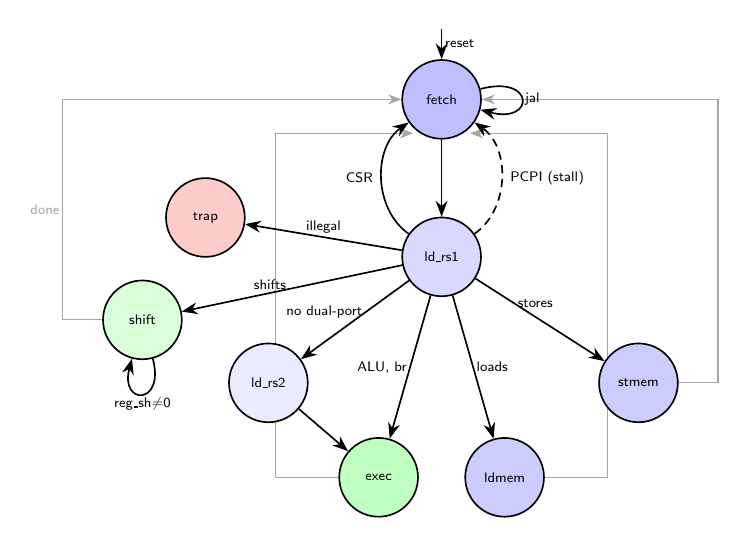
\begin{tikzpicture}[>=Stealth, semithick,
      every state/.style={draw, circle, minimum size=1.0cm,
                          font=\sffamily\tiny, inner sep=1pt, align=center},
      every edge/.style={draw, ->, >=Stealth},
      lbl/.style={font=\sffamily\tiny, inner sep=1pt}]

    % FSM state colors: blue=control flow, green=compute, blue(light)=memory, red=error
    % Layout: dispatch arrows go DOWN through the center;
    %         return arrows go UP along the LEFT and RIGHT margins to avoid crossing.

    % --- Row 0: fetch ---
    \node[state, fill=blue!25] (fetch) at (0, 0) {fetch};

    % --- Row 1: ld_rs1, ld_rs2 ---
    \node[state, fill=blue!15] (ldrs1) at (0, -2.0) {ld\_rs1};
    \node[state, fill=blue!8]  (ldrs2) at (-2.2, -3.6) {ld\_rs2};

    % --- Row 2: execute states, spread wide ---
    \node[state, fill=green!25] (exec)  at (-0.8, -4.8) {exec};
    \node[state, fill=green!15] (shift) at (-3.8, -2.8) {shift};
    \node[state, fill=blue!20]  (ldmem) at (0.8, -4.8) {ldmem};
    \node[state, fill=blue!20]  (stmem) at (2.5, -3.6) {stmem};
    \node[state, fill=red!20]    (trap)  at (-3, -1.5) {trap};

    % ======= DOWNWARD DISPATCH (center) =======

    % Reset
    \draw[->] (0, 0.9) -- (fetch) node[midway, right, lbl] {reset};

    % jal: self-loop
    \path (fetch) edge[loop right, looseness=7] node[right, lbl] {jal} (fetch);

    % fetch -> ld_rs1
    \draw[->] (fetch) -- (ldrs1) node[midway, left, lbl] {};

    % CSR: ld_rs1 -> fetch (solid, immediate, left side)
    \draw[->] (ldrs1) to[bend left=55] node[left, lbl, xshift=-2pt] {\tiny CSR} (fetch);
    % PCPI: ld_rs1 -> fetch (dashed, stalls until pcpi_ready, right side)
    \draw[->, densely dashed] (ldrs1) to[bend right=55] node[right, lbl, xshift=2pt] {\tiny PCPI (stall)} (fetch);

    % ld_rs1 dispatch (fan out)
    \draw[->] (ldrs1) -- (exec) node[pos=0.5, left, lbl] {ALU, br};
    \draw[->] (ldrs1) -- (ldmem) node[pos=0.5, right, lbl] {loads};
    \draw[->] (ldrs1) -- (stmem) node[pos=0.3, right, lbl] {stores};
    \draw[->] (ldrs1) -- (shift) node[pos=0.6, above, lbl] {shifts};
    \draw[->] (ldrs1) -- (trap) node[midway, above, lbl] {illegal};
    \draw[->] (ldrs1) -- (ldrs2) node[pos=0.4, left, lbl] {\tiny no dual-port};

    % ld_rs2 -> exec
    \draw[->] (ldrs2) -- (exec);

    % ======= UPWARD RETURN (outer edges, drawn on background layer) =======
    \begin{scope}[on background layer]
    % Left margin: shift -> fetch, exec -> fetch
    \draw[->, gray!70] (shift.west) -- ++(-0.5, 0) |- (fetch.west)
        node[pos=0.25, left, lbl] {done};
    \draw[->, gray!70] (exec.west) -- ++(-0.8, 0) |- ([yshift=-2pt]fetch.south west);

    % Right margin: ldmem -> fetch, stmem -> fetch
    \draw[->, gray!70] (ldmem.east) -- ++(0.8, 0) |- ([yshift=-2pt]fetch.south east);
    \draw[->, gray!70] (stmem.east) -- ++(0.5, 0) |- (fetch.east);
    \end{scope}

    % shift self-loop
    \path (shift) edge[loop below, looseness=6] node[below, lbl] {reg\_sh$\neq$0} (shift);

    \end{tikzpicture}
    \caption{picorv32 FSM. \textcolor{blue!60}{Blue} = memory/storage access (fetch, register read, load/store), \textcolor{green!50!black}{green} = compute (ALU, shift), \textcolor{red!60}{red} = error. Dispatch arrows (black) fan downward from \texttt{ld\_rs1}. Return arrows (grey) route along the outer edges back to \texttt{fetch}, avoiding crossings.}
    \label{fig:picorv32-fsm}
\end{figure}

\begin{table}[htbp]
\centering\small
\begin{tabular}{@{}l l l l c@{}}
    \toprule
    Class & Instructions & Fmt & Path & Cycles \\
    \midrule
    R-type ALU & \texttt{add}, \texttt{sub}, \texttt{and}, \texttt{or}, \texttt{slt} & R & fetch $\to$ ld\_rs1 $\to$ exec $\to$ (fetch) & 3 \\
    I-type ALU & \texttt{addi}, \texttt{andi}, \texttt{ori}, \texttt{slti} & I & fetch $\to$ ld\_rs1 $\to$ exec $\to$ (fetch) & 3 \\
    Upper imm. & \texttt{lui}, \texttt{auipc} & U & fetch $\to$ ld\_rs1 $\to$ exec $\to$ (fetch) & 3 \\
    Branch (not taken) & \texttt{beq}, \texttt{bne}, \texttt{blt}, \ldots & B & fetch $\to$ ld\_rs1 $\to$ exec $\to$ (fetch) & 3 \\
    Branch (taken) & \texttt{beq}, \texttt{bne}, \texttt{blt}, \ldots & B & fetch $\to$ ld\_rs1 $\to$ exec $\to$ refetch & 5 \\
    JALR & \texttt{jalr} & I & fetch $\to$ ld\_rs1 $\to$ exec $\to$ refetch & 6 \\
    JAL & \texttt{jal} & J & fetch $\to$ fetch & 3 \\
    \midrule
    Load & \texttt{lw}, \texttt{lh}, \texttt{lb}, \texttt{lhu}, \texttt{lbu} & I & fetch $\to$ ld\_rs1 $\to$ ldmem$^{\times 2}$ $\to$ fetch & 5 \\
    Store & \texttt{sw}, \texttt{sh}, \texttt{sb} & S & fetch $\to$ ld\_rs1 $\to$ stmem$^{\times 2}$ $\to$ fetch & 5 \\
    \midrule
    Shift (no barrel) & \texttt{sll}, \texttt{srl}, \texttt{sra}, \ldots & R/I & fetch $\to$ ld\_rs1 $\to$ shift$^{\times k}$ $\to$ (fetch) & 4--14 \\
    Shift (barrel) & (same, with \texttt{BARREL\_SHIFTER}=1) & R/I & fetch $\to$ ld\_rs1 $\to$ exec $\to$ (fetch) & 3 \\
    \midrule
    MUL (fast) & \texttt{mul}, \texttt{mulh}, \texttt{mulhsu}, \texttt{mulhu} & R & fetch $\to$ ld\_rs1\,(stall) $\to$ (fetch) & ${\sim}5$ \\
    DIV & \texttt{div}, \texttt{divu}, \texttt{rem}, \texttt{remu} & R & fetch $\to$ ld\_rs1\,(stall) $\to$ (fetch) & ${\sim}40$ \\
    CSR read & \texttt{rdcycle}, \texttt{rdinstr} & I & fetch $\to$ ld\_rs1 $\to$ (fetch) & 2 \\
    Illegal & (unrecognised) & --- & fetch $\to$ ld\_rs1 $\to$ trap & --- \\
    \bottomrule
\end{tabular}
\caption{picorv32 instruction paths and cycle counts (\texttt{ENABLE\_REGS\_DUALPORT}=1, single-cycle memory). The \emph{Path} column shows the CPU-FSM states traversed; the \emph{Cycles} column is the documented steady-state CPI (picorv32 README), which additionally accounts for the instruction-fetch handshake and prefetch overlap. Every path returns to \texttt{fetch}, where the instruction's deferred writeback occurs. A parenthesised \texttt{(fetch)} is overlapped with the next instruction via prefetch, so it costs nothing and is not counted; a \emph{plain} trailing \texttt{fetch} (loads, stores) is a real cycle the instruction owns, because the data access occupies the shared bus and blocks prefetching --- which is why loads and stores cost~5 rather than~3. A \emph{taken} branch or \texttt{jalr} likewise cannot use the (wrong-path) prefetch and must \emph{refetch} the real target, costing the extra cycles shown. Superscript $\times k$\,=\,state visited $k$ times (for shifts, $k$ depends on the shift amount with \texttt{TWO\_STAGE\_SHIFT}=1, giving 4--14 cycles). See Table~\ref{tab:picorv32-states} for each state.}
\label{tab:picorv32-cpi}
\end{table}

\paragraph{Deviations from textbook.} The textbook multicycle FSM (Harris~\S7.4) has separate Decode and Writeback states. picorv32 eliminates both to save cycles, using three techniques:

\begin{enumerate}
    \item \textbf{Deferred writeback.} There is no Writeback state. Instead, execute/load/store states set \emph{latched} control signals (\texttt{latched\_store}, \texttt{latched\_stalu} (``store ALU result''), \texttt{latched\_branch}, \texttt{latched\_rd}) recording what to write. The actual register file write happens at the \emph{beginning of the next} \texttt{fetch} cycle. This means \texttt{fetch} simultaneously writes the previous instruction's result and fetches the next instruction.

    \item \textbf{Overlapped decode.} Decoding is not a state --- it is triggered by signals from the memory interface. When an instruction word arrives (\texttt{mem\_done}), decoder Stage~1 fires immediately (opcode $\to$ group flags, extract rd/rs1/rs2). One cycle later, Stage~2 fires (funct3/funct7 $\to$ individual \texttt{instr\_*} flags, compute \texttt{decoded\_imm}). Stage~2 completes in the same cycle as \texttt{ld\_rs1}, so by the time \texttt{ld\_rs1} dispatches, all instruction flags are valid.

    \item \textbf{Speculative prefetch.} The memory interface has its own 4-state FSM running in parallel with the CPU FSM. While the CPU is in \texttt{ld\_rs1} or \texttt{exec}, it can speculatively prefetch the next instruction (\texttt{mem\_do\_prefetch}). If the PC advances sequentially, the prefetched instruction is ready immediately; if a branch is taken, the prefetch is discarded.
\end{enumerate}

\paragraph{Walkthrough: \texttt{lw t1, 8(s0)} (5 cycles).} or equivalently \texttt{t1  $\gets$  Memory[s0 + 8]}. Take the base address which is value of register \texttt{s0}, add 8 to it, read \texttt{Memory[s0+8]}, then store this value to register \texttt{t1}. A single load exercises all three mechanisms above at once --- \emph{overlapped decode}, \emph{speculative prefetch}, and \emph{deferred writeback} --- and shows why it is one of the most expensive common instructions (only \texttt{jalr}/\texttt{ret} at~6, and the multi-cycle M-extension, cost more):

\begin{center}\small
\renewcommand{\arraystretch}{1.35}
\begin{tabular}{@{}c l p{9.5cm}@{}}
    \toprule
    Cyc & State & What happens \\
    \midrule
    1 & \texttt{fetch} &
        The instruction word arrives. In the \emph{same} cycle the CPU writes back the \emph{previous} instruction's result (deferred writeback). Decoder Stage~1 fires: opcode bits activate flag \texttt{is\_lb\_lh\_lw\_lbu\_lhu$\gets$1}, extracting \texttt{decoded\_rs1$\gets$8} since register s0 is \texttt{x8} and \texttt{decoded\_rd$\gets$6} since register t1 is \texttt{x6}. It also \emph{launches a prefetch} of the next sequential instruction. \\
    \midrule
    2 & \texttt{ld\_rs1} &
        Decoder Stage~2 resolves \texttt{funct3} as \texttt{instr\_lw$\gets$1} and the immediate \texttt{decoded\_imm$\gets$8}. The value of s0 (which is an address) at base register is read into a working register: \texttt{reg\_op1 $\leftarrow$ cpuregs[8]}. \\
    \midrule
    3 & \texttt{ldmem} &
        \emph{First visit.} An adder computes the effective address \texttt{reg\_op1 $\leftarrow$ reg\_op1 + decoded\_imm} (= s0+8), and \texttt{set\_mem\_do\_rdata} issues the \emph{data} read on the shared bus. While this read is in flight, no instruction can be prefetched. \\
    \midrule
    4 & \texttt{ldmem} &
        \emph{Second visit.} The data returns (\texttt{mem\_done}); the aligned word is captured into \texttt{reg\_out $\leftarrow$ mem\_rdata\_word} (a full word for \texttt{lw}; \texttt{lh}/\texttt{lb} would sign-extend, \texttt{lhu}/\texttt{lbu} zero-extend). \texttt{latched\_store $\leftarrow$ 1} flags the pending writeback. \\
    \midrule
    5 & \texttt{fetch} &
        Back in \texttt{fetch}: the deferred writeback completes (\texttt{cpuregs[6] $\leftarrow$ reg\_out}, so t1 now holds the word) \emph{and} the next instruction is fetched and decoded. For an ALU op this fetch would be free --- its successor was prefetched during \texttt{exec} --- but here it is a \emph{real} cycle, because the data access in cycles~3--4 left no bus bandwidth to prefetch. \\
    \bottomrule
\end{tabular}
\end{center}

So the load costs 5 cycles for two compounding reasons: \texttt{ldmem} is entered \emph{twice} (cycle~3 computes the address and starts the read; cycle~4 waits for the data), and its trailing \texttt{fetch} (cycle~5) is a \emph{real} cycle rather than a free overlap, since the in-flight data access blocked the prefetch. An ALU instruction avoids both: it has a single \texttt{exec} step and prefetches its successor, so it finishes in \texttt{fetch $\to$ ld\_rs1 $\to$ exec} (3 cycles) with its writeback folded into the next instruction's fetch --- the parenthesised \texttt{(fetch)} in Table~\ref{tab:picorv32-cpi}.

\newpage
\subsection{Datapath}

Figure~\ref{fig:picorv32-datapath} shows the picorv32 datapath. Like the textbook multicycle processor (Harris Figure~7.27), it consists of state elements connected by nonarchitectural registers and multiplexers that route data differently on each FSM step.


\begin{figure}[htbp]
    \centering
    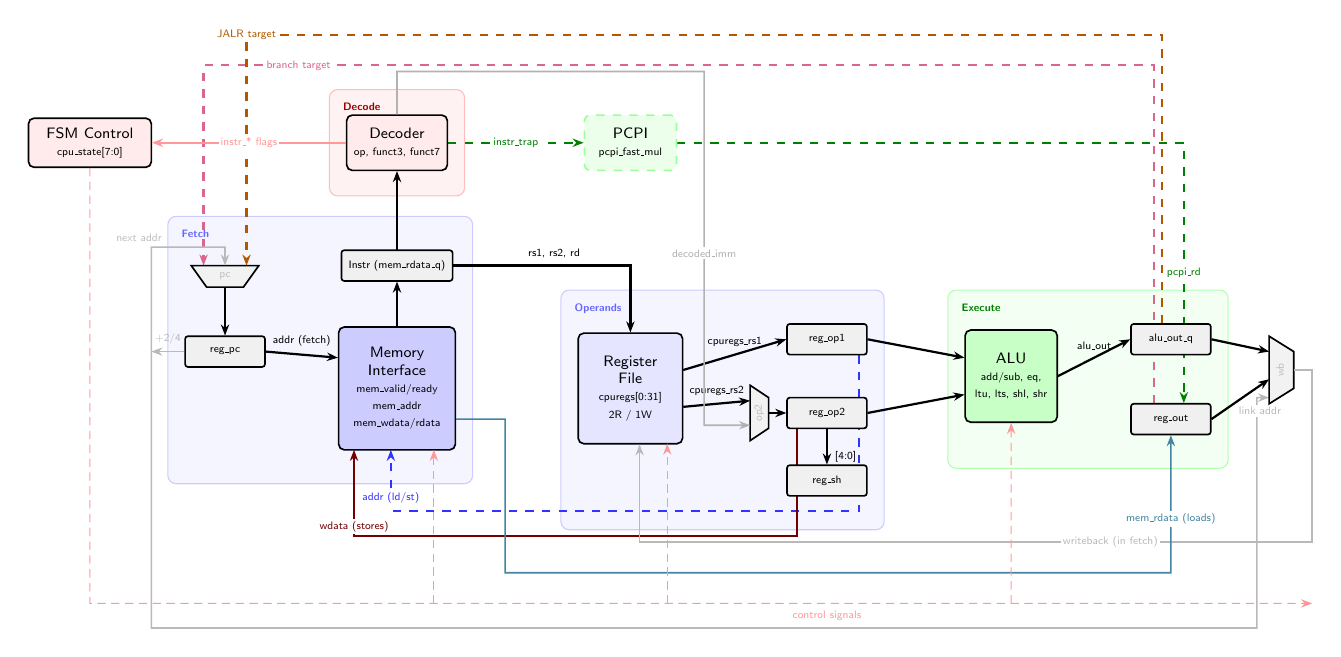
\begin{tikzpicture}[>=Stealth, semithick, scale=0.78, every node/.style={transform shape},
      blk/.style={draw, rounded corners=2pt, minimum height=0.9cm,
                  minimum width=1.6cm, font=\sffamily\scriptsize, align=center},
      reg/.style={draw, fill=gray!12, rounded corners=1pt, minimum height=0.5cm,
                  minimum width=1.3cm, font=\sffamily\tiny, align=center},
      arr/.style={-{Stealth[length=4pt, width=3pt]}, thick},
      fb/.style={-{Stealth[length=4pt, width=3pt]}, semithick},
      ctrl/.style={-{Stealth[length=4pt, width=3pt]}, red!40, thin},
      lbl/.style={font=\sffamily\tiny},
      flbl/.style={font=\sffamily\tiny, fill=white, inner sep=1pt}]

    % ============================
    % NODES
    % ============================
    \node[reg] (pc) at (-2.8, 0.6) {reg\_pc};

    % PC mux (3-input: branch target, sequential, JALR target)
    \fill[gray!10] (-3.35, 2.0) -- (-3.1, 1.65) -- (-2.5, 1.65) -- (-2.25, 2.0) -- cycle;
    \draw (-3.35, 2.0) -- (-3.1, 1.65) -- (-2.5, 1.65) -- (-2.25, 2.0) -- cycle;
    \node[font=\sffamily\tiny, text=gray!50] at (-2.8, 1.82) {pc};
    \coordinate (pcmux-n-left) at (-3.15, 2.0);   % branch target
    \coordinate (pcmux-n-mid) at (-2.8, 2.0);     % sequential (reg_next_pc)
    \coordinate (pcmux-n-right) at (-2.45, 2.0);  % JALR target
    \coordinate (pcmux-south) at (-2.8, 1.65);
    \draw[arr] (pcmux-south) -- (pc.north);

    % +2/4 fork: reg_pc -> fork point, then splits to PC mux (seq) and WB mux (link)
    \coordinate (pcfork) at (-4.0, 0.6);
    \draw[fb, gray!55] (pc.west) -- (pcfork) node[midway, above, font=\sffamily\tiny] {+2/4};
    % Fork up: to PC mux sequential input
    \draw[fb, gray!55] (pcfork) -- (-4.0, 2.3) -- (-2.8, 2.3) -- (pcmux-n-mid);
    \node[flbl, text=gray!50] at (-4.2, 2.45) {next addr};

    \node[blk, fill=blue!20, minimum height=2.0cm, minimum width=1.9cm] (mem) at (0, 0)
      {Memory\\Interface\\{\tiny mem\_valid/ready}\\{\tiny mem\_addr}\\{\tiny mem\_wdata/rdata}};

    \node[reg] (ir) at (0, 2.0) {Instr (mem\_rdata\_q)};

    \node[blk, fill=red!8, minimum width=1.5cm] (dec) at (0, 4.0)
      {Decoder\\{\tiny op, funct3, funct7}};

    \node[blk, fill=blue!10, minimum height=1.8cm, minimum width=1.7cm] (rf) at (3.8, 0)
      {Register\\File\\{\tiny cpuregs[0:31]}\\{\tiny 2R / 1W}};

    \node[reg] (op1) at (7.0, 0.8)  {reg\_op1};
    \node[reg] (op2) at (7.0, -0.4) {reg\_op2};
    \node[reg] (sh)  at (7.0, -1.5) {reg\_sh};

    \node[blk, fill=green!22, minimum height=1.5cm, minimum width=1.5cm] (alu) at (10.0, 0.2)
      {ALU\\{\tiny add/sub, eq,}\\{\tiny ltu, lts, shl, shr}};

    \node[reg] (aluq) at (12.6, 0.8) {alu\_out\_q};
    \node[reg] (rout) at (12.6, -0.5) {reg\_out};

    % Writeback mux (3-input: alu_out_q and reg_out from left, link addr from bottom)
    \fill[gray!10] (14.2, 0.85) -- (14.6, 0.6) -- (14.6, 0.0) -- (14.2, -0.25) -- cycle;
    \draw (14.2, 0.85) -- (14.6, 0.6) -- (14.6, 0.0) -- (14.2, -0.25) -- cycle;
    \node[font=\sffamily\tiny, text=gray!50, rotate=90] at (14.38, 0.3) {wb};
    \coordinate (wbmux-w-top) at (14.2, 0.6);    % alu_out_q
    \coordinate (wbmux-w-bot) at (14.2, 0.15);   % reg_out
    \coordinate (wbmux-w-link) at (14.2, -0.15);  % link addr (lowest left input)
    \coordinate (wbmux-east) at (14.6, 0.3);

    % ============================
    % PCPI coprocessor (top right of decoder)
    % ============================
    \node[blk, fill=green!8, minimum width=1.5cm, dashed, draw=green!40]
      (pcpi) at (3.8, 4.0) {PCPI\\{\tiny pcpi\_fast\_mul}};
    \draw[arr, green!50!black, dashed] (dec.east) -- (pcpi.west)
      node[midway, flbl, text=green!50!black] {instr\_trap};

    % ============================
    % BACKGROUND: stage boxes, feedback paths that go behind nodes
    % ============================
    \begin{scope}[on background layer]
    \node[draw=blue!20, rounded corners=3pt, inner sep=6pt, inner ysep=12pt, fill=blue!4,
          fit=(pc)(mem)(ir)] (fetchbox) {};
    \node[draw=red!25, rounded corners=3pt, inner sep=6pt, inner ysep=9pt, fill=red!5,
          fit=(dec)] (decodebox) {};
    \node[draw=blue!20, rounded corners=3pt, inner sep=6pt, inner ysep=12pt, fill=blue!4,
          fit=(rf)(op1)(op2)(sh)] (operandsbox) {};
    \node[draw=green!30, rounded corners=3pt, inner sep=6pt, inner ysep=12pt, fill=green!5,
          fit=(alu)(aluq)(rout)] (executebox) {};

    % Branch target: reg_out -> PC mux (conditional branches)
    \draw[fb, purple!60, dashed, thick] ([xshift=-8pt]rout.north) -- ++(0, 5.5)
      -| (pcmux-n-left)
      node[pos=0.45, flbl, text=purple!60] {branch target};
    % JALR target: alu_out_q -> PC mux (register-indirect jump)
    \draw[fb, orange!70!black, dashed, thick] ([xshift=-4pt]aluq.north) -- ++(0, 4.7)
      -| (pcmux-n-right)
      node[pos=0.5, flbl, text=orange!70!black] {JALR target};
    % PCPI result -> reg_out ---
    \draw[fb, green!50!black, dashed, thick] (pcpi.east) -- ([xshift=6pt]rout.north |- pcpi.east) -- ([xshift=6pt]rout.north)
      node[pos=0.5, flbl, text=green!50!black] {pcpi\_rd};
    \end{scope}

    % Stage labels (foreground so they render on top of the fill)
    \node[font=\sffamily\tiny\bfseries, blue!60, anchor=north west] at ([xshift=3pt, yshift=-3pt]fetchbox.north west) {Fetch};
    \node[font=\sffamily\tiny\bfseries, red!60!black, anchor=north west] at ([xshift=3pt, yshift=-3pt]decodebox.north west) {Decode};
    \node[font=\sffamily\tiny\bfseries, blue!60, anchor=north west] at ([xshift=3pt, yshift=-3pt]operandsbox.north west) {Operands};
    \node[font=\sffamily\tiny\bfseries, green!50!black, anchor=north west] at ([xshift=3pt, yshift=-3pt]executebox.north west) {Execute};

    % ============================
    % FORWARD DATAPATH (left to right)
    % ============================
    \draw[arr] (pc.east) -- ([yshift=0.5cm]mem.west)
      node[midway, above, lbl] {addr (fetch)};
    \draw[arr] (mem.north) -- (ir.south);
    \draw[arr] (ir.north) -- (dec.south);
    \draw[arr] (ir.east) -- ++(0.4, 0) -| (rf.north)
      node[pos=0.25, above, lbl] {rs1, rs2, rd};
    \draw[arr] ([yshift=0.3cm]rf.east) -- (op1.west)
      node[midway, above, lbl] {cpuregs\_rs1};

    % reg_op2 mux (trapezoid)
    \fill[gray!10] (5.75, 0.05) -- (6.05, -0.15) -- (6.05, -0.65) -- (5.75, -0.85) -- cycle;
    \draw (5.75, 0.05) -- (6.05, -0.15) -- (6.05, -0.65) -- (5.75, -0.85) -- cycle;
    \node[font=\sffamily\tiny, text=gray!50, rotate=90] at (5.9, -0.4) {op2};
    \coordinate (op2mux-w-top) at (5.75, -0.2);
    \coordinate (op2mux-w-bot) at (5.75, -0.6);
    \coordinate (op2mux-east) at (6.05, -0.4);

    \draw[arr] ([yshift=-0.3cm]rf.east) -- (op2mux-w-top)
      node[midway, above, lbl] {cpuregs\_rs2};
    \draw[arr] (op2mux-east) -- (op2.west);
    \draw[fb, gray!60] (dec.north) -- ++(0, 0.7) -| (5.0, -0.6) -- (op2mux-w-bot);
    \node[flbl, text=gray!60] at (5.0, 2.2) {decoded\_imm};

    % reg_op2 -> reg_sh
    \draw[arr] (op2.south) -- ++(0, -0.45) -| (sh.north)
      node[pos=0.0, right, lbl] {[4:0]};

    % Working registers -> ALU
    \draw[arr] (op1.east) -- ([yshift=0.3cm]alu.west);
    \draw[arr] (op2.east) -- ([yshift=-0.3cm]alu.west);

    % ALU -> alu_out_q
    \draw[arr] (alu.east) -- (aluq.west)
      node[midway, above, lbl] {alu\_out};

    % alu_out_q -> writeback mux (top-left input)
    \draw[arr] (aluq.east) -- (wbmux-w-top);
    % reg_out -> writeback mux (bottom-left input)
    \draw[arr] (rout.east) -- (wbmux-w-bot);

    % Fork down: from +2/4 fork point, along bottom, up to WB mux (link addr from below)
    \begin{scope}[on background layer]
    \draw[fb, gray!55] (pcfork) -- (-4.0, -3.9)
      -- (14.0, -3.9) -- (14.0, -0.15) -- (wbmux-w-link)
      node[pos=0.25, below=3pt, flbl] {link addr};
    \end{scope}

    % ============================
    % FEEDBACK PATHS (foreground)
    % ============================

    % (B) Writeback: wb mux -> RF
    \draw[fb, gray!55] (wbmux-east) -- ++(0.3, 0) -- ++(0, -2.8)
      -| ([xshift=0.15cm]rf.south)
      node[pos=0.15, flbl] {writeback (in fetch)};

    % (C) Data address: reg_op1 south, behind op2/sh (background layer), left, up to Memory
    \begin{scope}[on background layer]
    \draw[fb, blue!80, dashed] ([xshift=15pt]op1.south) -- ([xshift=15pt]op1.south |- 0,-2.0)
      -- (-0.1, -2.0) -- (-0.1, -1.0)
      node[pos=0.35, below, flbl, text=blue!80] {addr (ld/st)};
    \end{scope}

    % (D) Store data: reg_op2 south, behind sh, down, left, up to Memory
    \begin{scope}[on background layer]
    \draw[fb, red!45!black] ([xshift=-14pt]op2.south) -- ([xshift=-14pt]op2.south |- 0,-2.4)
      -- (-0.7, -2.4) -- (-0.7, -1.0)
      node[pos=0.2, below, flbl, text=red!45!black] {wdata (stores)};
    \end{scope}

    % (E) Load data: Memory -> reg_out (horizontal below writeback line, then up)
    \draw[fb, cyan!60!black] ([yshift=-0.5cm]mem.east) -- ++(0.8, 0) -- ++(0, -2.5)
      -- (12.6, -3.0) -- (rout.south)
      node[pos=0.45, below, flbl, text=cyan!60!black] {mem\_rdata (loads)};

    % ============================
    % FSM CONTROL UNIT
    % ============================
    \node[blk, fill=red!8, minimum height=0.8cm, minimum width=2.0cm,
          font=\sffamily\scriptsize] (fsm) at (-5.0, 4.0)
      {FSM Control\\{\tiny cpu\_state[7:0]}};

    \draw[arr, red!40] (dec.west) -- (fsm.east)
      node[midway, flbl, text=red!40] {instr\_* flags};

    % FSM control bus (taps shifted right to avoid blue/red lines)
    \draw[ctrl, densely dashed] (fsm.south) -- (-5.0, -3.5) -- (14.9, -3.5);
    \draw[ctrl, densely dashed] (0.6, -3.5) -- (0.6, -1.0);
    \draw[ctrl, densely dashed] (4.4, -3.5) -- (4.4, -0.9);
    \draw[ctrl, densely dashed] (10.0, -3.5) -- (alu.south);
    \node[flbl, text=red!40] at (7.0, -3.7) {control signals};

    \end{tikzpicture}
    \caption{Simplified picorv32 datapath (v2). Three multiplexers control data routing: the \textbf{op2 mux} selects the ALU's second operand, the \textbf{writeback (wb) mux} selects what is written to the register file, and the \textbf{PC mux} selects the next instruction address. A \textbf{+2/4 fork} (+2 for \texttt{COMPRESSED\_ISA} and +4 for full 32bit addresses) from \texttt{reg\_pc} computes the next sequential address and feeds both the PC mux (as the default ``next addr'') and the writeback mux (as the ``link addr'' for JAL/JALR return addresses; note this is a separate adder, not the ALU).
    \textbf{Forward path} (black): PC $\to$ Memory Interface $\to$ Instruction Register $\to$ Decoder (one-hot flags) and Register File (rs1/rs2/rd indices). \texttt{reg\_op1} receives \texttt{cpuregs\_rs1}; \texttt{reg\_op2} receives \texttt{cpuregs\_rs2} or \texttt{decoded\_imm} via the op2 mux. Both feed the ALU; its combinational output is registered into \texttt{alu\_out\_q} every cycle.
    \textbf{Feedback paths}: \textcolor{purple!60}{purple dashed} = branch target (\texttt{reg\_out} $\to$ PC mux); \textcolor{orange!70!black}{orange dashed} = JALR target (\texttt{alu\_out\_q} $\to$ PC mux); \textcolor{cyan!60!black}{teal} = load data (\texttt{mem\_rdata} $\to$ \texttt{reg\_out}); \textcolor{red!45!black}{red} = store data (\texttt{reg\_op2} $\to$ memory); \textcolor{blue!80}{blue dashed} = data address (\texttt{reg\_op1 + decoded\_imm} $\to$ memory); \textcolor{green!50!black}{green dashed} = PCPI (\texttt{pcpi\_rd} $\to$ \texttt{reg\_out}); grey = +2/4 fork (\texttt{reg\_pc} $\to$ PC mux and writeback mux). Not shown: in the \texttt{shift} state, \texttt{reg\_op1} is shifted in-place (1 or 4 bits/cycle) and \texttt{reg\_sh} is decremented until zero.}
    \label{fig:picorv32-datapath}
\end{figure}

\paragraph{Architectural state.} In standalone \texttt{picorv32.v} the processor's permanent state is the 32-entry $\times$ 32-bit register file and the program counter (\texttt{reg\_pc}). In standalone \texttt{picorv32}, the register file is a Verilog 2D array (\texttt{reg [31:0] cpuregs [0:regfile\_size-1]}). Each cycle, \texttt{decoded\_rs1} and \texttt{decoded\_rs2} holds the address index of the decoded rs1 and rs2 registers. Two combinational read-port wires (\texttt{cpuregs\_rs1}, \texttt{cpuregs\_rs2}) hold the value of these addresses, returning 0 when the index is 0 (the x0 convention). Writes are gated by \texttt{latched\_rd $\neq$ 0}.

\paragraph{Nonarchitectural working registers.} These hold intermediate results between FSM states:
\begin{itemize}
    \item \textbf{\texttt{reg\_op1}}: first ALU input (loaded from \texttt{cpuregs\_rs1} in \texttt{ld\_rs1}).\footnote{\texttt{cpuregs\_rs1} is a combinational wire that reads \texttt{cpuregs[decoded\_rs1]} --- it gives the current \emph{value} stored in the rs1 register. Because it is combinational, it changes instantly whenever \texttt{decoded\_rs1} changes (i.e.\ when the next instruction is decoded). \texttt{reg\_op1} is a clocked flip-flop that \emph{latches} this value so it remains stable across subsequent FSM states. Without the latch, the ALU or memory interface would see the wrong register's contents once the decoder moves on to the next instruction.} Repurposed during \texttt{ldmem}/\texttt{stmem}: the FSM overwrites it with \texttt{reg\_op1 + decoded\_imm} (i.e.\ base + offset), so it then holds the computed data memory address that feeds \texttt{mem\_la\_addr}.
    \item \textbf{\texttt{reg\_op2}}: second ALU input --- either \texttt{cpuregs\_rs2} (R-type) or \texttt{decoded\_imm} (I-type). This mux is the key difference between register--register and register--immediate instructions.
    \item \textbf{\texttt{reg\_out}}: general result register for non-ALU results: loaded data (\texttt{mem\_rdata\_word} in \texttt{ldmem}), shifted value (\texttt{reg\_op1} in \texttt{shift}), PCPI result (\texttt{pcpi\_int\_rd}), CSR values, and branch target (\texttt{reg\_pc + decoded\_imm} in \texttt{exec}). \emph{Not} the ALU output --- see \texttt{alu\_out\_q} below.
    \item \textbf{\texttt{alu\_out\_q}}: registered copy of the ALU output, updated every cycle (\texttt{alu\_out\_q <= alu\_out}). This is the writeback source for ALU instructions (add, sub, and, or, slt, etc.), selected by \texttt{latched\_stalu}.
    \item \textbf{\texttt{reg\_sh}}: 5-bit shift counter for iterative shifts (decremented each cycle in \texttt{shift} state).
\end{itemize}

At writeback time (beginning of \texttt{fetch}), a mux selects the register file write data:
\begin{center}\small
\begin{tabular}{@{}l l l@{}}
    \toprule
    Condition & \texttt{cpuregs\_wrdata} & Used by \\
    \midrule
    \texttt{latched\_branch} & \texttt{reg\_pc + 2/4} & JAL/JALR link address \\
    \texttt{latched\_stalu} & \texttt{alu\_out\_q} & ALU instructions \\
    otherwise & \texttt{reg\_out} & Loads, shifts, CSRs, PCPI \\
    \bottomrule
\end{tabular}
\end{center}

\paragraph{ALU.} The ALU computes six operations in parallel from \texttt{reg\_op1} and \texttt{reg\_op2}. By default these are combinational; with \texttt{TWO\_CYCLE\_ALU}=1 they become registered (adds one cycle latency, shortens critical path):

\begin{center}\small
\begin{tabular}{@{}l l@{}}
    \toprule
    Signal & Operation \\
    \midrule
    \texttt{alu\_add\_sub} & \texttt{reg\_op1 $\pm$ reg\_op2} (add/sub, also used for address calc and LUI/AUIPC) \\
    \texttt{alu\_eq}, \texttt{alu\_lts}, \texttt{alu\_ltu} & equality, signed less-than, unsigned less-than (for branches and SLT) \\
    \texttt{alu\_shl}, \texttt{alu\_shr} & left/right shift (used only when \texttt{BARREL\_SHIFTER}=1) \\
    \bottomrule
\end{tabular}
\end{center}

An output mux selects the final 32-bit result (\texttt{alu\_out}) based on the instruction type: \texttt{alu\_add\_sub} for arithmetic/address operations, comparison flags for branches/SLT, XOR/OR/AND for logical operations, or shift results when barrel-shifting is enabled. This combinational result is registered into \texttt{alu\_out\_q} every cycle.

\subsection{Instruction decoder}

Unlike the textbook decoder (Harris~\S7.3.3), which produces abstract control signals (RegWrite, ALUSrc, etc.), picorv32 sets \textbf{one-hot instruction flags} (\texttt{instr\_add}, \texttt{instr\_beq}, \texttt{instr\_lw}, etc.) that the FSM tests directly. The decode is split across two clock edges:

\paragraph{Stage 1: opcode grouping.} Triggered when a new instruction word arrives from memory (\texttt{mem\_do\_rinst} (``read instruction'') \texttt{\&\& mem\_done}), Stage~1 examines \texttt{opcode[6:0]} from the raw instruction word and classifies it into one of nine opcode groups. It simultaneously extracts the register indices (\texttt{decoded\_rd} from \texttt{[11:7]}, \texttt{decoded\_rs1} from \texttt{[19:15]}, \texttt{decoded\_rs2} from \texttt{[24:20]}) and pre-computes the J-type immediate \texttt{decoded\_imm\_j}.

\paragraph{Stage 2: funct3/funct7 refinement.} Triggered one cycle later by \texttt{decoder\_trigger}, Stage~2 combines the group flags with \texttt{funct3[14:12]} and (for R-type) \texttt{funct7[31:25]} to set individual one-hot instruction signals \texttt{instr\_*}. Stage~2 also computes the final \texttt{decoded\_imm} via a format-dependent case statement (Section~\ref{sec:isa}, Figure~\ref{fig:rv32-formats}).

Table~\ref{tab:decode-unified} shows the complete two-stage decode: Stage~1 maps the opcode to a group flag (left columns), then Stage~2 refines each group by funct3/funct7 into the final \texttt{instr\_*} signal (right columns). LUI, AUIPC, JAL, and JALR are fully resolved in Stage~1 and need no Stage~2 refinement.

\begin{table}[htbp]
\centering\footnotesize
\renewcommand{\arraystretch}{1.10}
\begin{tabular*}{\textwidth}{@{\extracolsep{\fill}} l l l | l l l l l p{2.5cm} @{}}
    \toprule
    \multicolumn{3}{c|}{Stage~1 (opcode)} & \multicolumn{6}{c}{Stage~2 (funct3 / funct7)} \\
    \texttt{opcode} & Group flag & Fmt & \texttt{f3} & \texttt{f7} & Signal & Asm & RTL & Description \\
    \midrule
    \texttt{0110111} & \texttt{instr\_lui}   & U & --- & --- & \texttt{instr\_lui}   & \texttt{lui}   & \texttt{rd $\leftarrow$ imm $\ll$ 12}       & Load upper immediate \\
    \texttt{0010111} & \texttt{instr\_auipc} & U & --- & --- & \texttt{instr\_auipc} & \texttt{auipc} & \texttt{rd $\leftarrow$ PC+(imm$\ll$12)}    & Add upper imm to PC \\
    \texttt{1101111} & \texttt{instr\_jal}   & J & --- & --- & \texttt{instr\_jal}   & \texttt{jal}   & \texttt{rd $\leftarrow$ PC+4; PC+=imm}      & Jump and link \\
    \texttt{1100111} & \texttt{instr\_jalr}  & I & \texttt{000} & --- & \texttt{instr\_jalr}  & \texttt{jalr}  & \texttt{rd $\leftarrow$ PC+4; PC $\leftarrow$ rs1+imm} & Jump and link register \\
    \midrule
    \texttt{1100011} & \texttt{is\_beq\_bne\_blt\_} & B
        & \texttt{000} & --- & \texttt{instr\_beq}  & \texttt{beq}  & \texttt{if(rs1==rs2) PC+=imm} & Branch if equal \\
    & \texttt{bge\_bltu\_bgeu} &
        & \texttt{001} & --- & \texttt{instr\_bne}  & \texttt{bne}  & \texttt{if(rs1!=rs2) PC+=imm} & Branch if not equal \\
    & &
        & \texttt{100} & --- & \texttt{instr\_blt}  & \texttt{blt}  & \texttt{if(rs1<rs2) PC+=imm}  & Branch if $<$ (signed) \\
    & &
        & \texttt{101} & --- & \texttt{instr\_bge}  & \texttt{bge}  & \texttt{if(rs1>=rs2) PC+=imm} & Branch if $\geq$ (signed) \\
    & &
        & \texttt{110} & --- & \texttt{instr\_bltu} & \texttt{bltu} & \texttt{if(rs1<rs2) PC+=imm}  & Branch if $<$ (unsigned) \\
    & &
        & \texttt{111} & --- & \texttt{instr\_bgeu} & \texttt{bgeu} & \texttt{if(rs1>=rs2) PC+=imm} & Branch if $\geq$ (unsigned) \\
    \midrule
    \texttt{0000011} & \texttt{is\_lb\_lh\_lw\_} & I
        & \texttt{000} & --- & \texttt{instr\_lb}  & \texttt{lb}  & \texttt{rd $\leftarrow$ sext(M[8])}  & Load byte, sign-extend \\
    & \texttt{lbu\_lhu} &
        & \texttt{001} & --- & \texttt{instr\_lh}  & \texttt{lh}  & \texttt{rd $\leftarrow$ sext(M[16])} & Load half, sign-extend \\
    & &
        & \texttt{010} & --- & \texttt{instr\_lw}  & \texttt{lw}  & \texttt{rd $\leftarrow$ M[32]}       & Load word \\
    & &
        & \texttt{100} & --- & \texttt{instr\_lbu} & \texttt{lbu} & \texttt{rd $\leftarrow$ zext(M[8])}  & Load byte, zero-extend \\
    & &
        & \texttt{101} & --- & \texttt{instr\_lhu} & \texttt{lhu} & \texttt{rd $\leftarrow$ zext(M[16])} & Load half, zero-extend \\
    \midrule
    \texttt{0100011} & \texttt{is\_sb\_sh\_sw} & S
        & \texttt{000} & --- & \texttt{instr\_sb} & \texttt{sb} & \texttt{M[8] $\leftarrow$ rs2}  & Store byte \\
    & &
        & \texttt{001} & --- & \texttt{instr\_sh} & \texttt{sh} & \texttt{M[16] $\leftarrow$ rs2} & Store halfword \\
    & &
        & \texttt{010} & --- & \texttt{instr\_sw} & \texttt{sw} & \texttt{M[32] $\leftarrow$ rs2} & Store word \\
    \midrule
    \texttt{0010011} & \texttt{is\_alu\_reg\_imm} & I
        & \texttt{000} & ---          & \texttt{instr\_addi}  & \texttt{addi}  & \texttt{rd $\leftarrow$ rs1+imm}          & Add immediate \\
    & &
        & \texttt{010} & ---          & \texttt{instr\_slti}  & \texttt{slti}  & \texttt{rd $\leftarrow$ (rs1<imm)?1:0}     & Set if $<$ imm (signed) \\
    & &
        & \texttt{011} & ---          & \texttt{instr\_sltiu} & \texttt{sltiu} & \texttt{rd $\leftarrow$ (rs1<imm)?1:0}     & Set if $<$ imm (unsign) \\
    & &
        & \texttt{100} & ---          & \texttt{instr\_xori}  & \texttt{xori}  & \texttt{rd $\leftarrow$ rs1\^{}imm}        & XOR immediate \\
    & &
        & \texttt{110} & ---          & \texttt{instr\_ori}   & \texttt{ori}   & \texttt{rd $\leftarrow$ rs1|imm}           & OR immediate \\
    & &
        & \texttt{111} & ---          & \texttt{instr\_andi}  & \texttt{andi}  & \texttt{rd $\leftarrow$ rs1\&imm}          & AND immediate \\
    & &
        & \texttt{001} & \texttt{0000000}  & \texttt{instr\_slli}  & \texttt{slli}  & \texttt{rd $\leftarrow$ rs1$\ll$shamt}     & Shift left logical imm \\
    & &
        & \texttt{101} & \texttt{0000000}  & \texttt{instr\_srli}  & \texttt{srli}  & \texttt{rd $\leftarrow$ rs1$\gg$shamt}     & Shift right logical imm \\
    & &
        & \texttt{101} & \texttt{0100000}  & \texttt{instr\_srai}  & \texttt{srai}  & \texttt{rd $\leftarrow$ rs1$\ggg$shamt}    & Shift right arith imm \\
    \midrule
    \texttt{0110011} & \texttt{is\_alu\_reg\_reg} & R
        & \texttt{000} & \texttt{0000000}  & \texttt{instr\_add}  & \texttt{add}  & \texttt{rd $\leftarrow$ rs1+rs2}          & Add \\
    & &
        & \texttt{000} & \texttt{0100000}  & \texttt{instr\_sub}  & \texttt{sub}  & \texttt{rd $\leftarrow$ rs1$-$rs2}        & Subtract \\
    & &
        & \texttt{001} & \texttt{0000000}  & \texttt{instr\_sll}  & \texttt{sll}  & \texttt{rd $\leftarrow$ rs1$\ll$rs2}      & Shift left logical \\
    & &
        & \texttt{010} & \texttt{0000000}  & \texttt{instr\_slt}  & \texttt{slt}  & \texttt{rd $\leftarrow$ (rs1<rs2)?1:0}    & Set if $<$ (signed) \\
    & &
        & \texttt{011} & \texttt{0000000}  & \texttt{instr\_sltu} & \texttt{sltu} & \texttt{rd $\leftarrow$ (rs1<rs2)?1:0}    & Set if $<$ (unsigned) \\
    & &
        & \texttt{100} & \texttt{0000000}  & \texttt{instr\_xor}  & \texttt{xor}  & \texttt{rd $\leftarrow$ rs1\^{}rs2}       & XOR \\
    & &
        & \texttt{101} & \texttt{0000000}  & \texttt{instr\_srl}  & \texttt{srl}  & \texttt{rd $\leftarrow$ rs1$\gg$rs2}      & Shift right logical \\
    & &
        & \texttt{101} & \texttt{0100000}  & \texttt{instr\_sra}  & \texttt{sra}  & \texttt{rd $\leftarrow$ rs1$\ggg$rs2}     & Shift right arithmetic \\
    & &
        & \texttt{110} & \texttt{0000000}  & \texttt{instr\_or}   & \texttt{or}   & \texttt{rd $\leftarrow$ rs1|rs2}          & OR \\
    & &
        & \texttt{111} & \texttt{0000000}  & \texttt{instr\_and}  & \texttt{and}  & \texttt{rd $\leftarrow$ rs1\&rs2}         & AND \\
    \bottomrule
\end{tabular*}
\caption{Unified picorv32 instruction decode table. Stage~1 (left of vertical rule) maps \texttt{opcode[6:0]} to a group flag on the first clock edge; Fmt shows the instruction format (R/I/S/B/U/J from Figure~\ref{fig:rv32-formats}). The first four instructions (LUI, AUIPC, JAL, JALR) are fully resolved in Stage~1. Stage~2 (right) refines each remaining group by \texttt{funct3} (3-bit) and \texttt{funct7} (7-bit, \texttt{instr[31:25]}) on the next clock edge; ``---'' means that field is not checked. M[$n$] denotes an $n$-bit memory access at address \texttt{rs1+imm}. The M~extension (mul/div) shares the R-type opcode \texttt{0110011} with \texttt{funct7}=\texttt{0000001}; since the base decoder does not recognise this funct7, \texttt{instr\_trap} fires and the instruction is forwarded to PCPI (Table~\ref{tab:m-ext}, Section~\ref{sec:pcpi}).}
\label{tab:decode-unified}
\end{table}

\paragraph{Worked example: \texttt{add x18, x19, x20}.} The 32-bit encoding \texttt{0x01498933} gives in binary form
\[
\underbrace{\texttt{0000000}}_{\text{funct7}}\,
\underbrace{\texttt{10100}}_{\text{rs2}=x20}\,
\underbrace{\texttt{10011}}_{\text{rs1}=x19}\,
\underbrace{\texttt{000}}_{\text{funct3}}\,
\underbrace{\texttt{10010}}_{\text{rd}=x18}\,
\underbrace{\texttt{0110011}}_{\text{opcode}}
\]
Stage~1 sees opcode \texttt{0110011} and sets \texttt{is\_alu\_reg\_reg $\leftarrow$ 1}, \texttt{decoded\_rs1 $\leftarrow$ 19}, \texttt{decoded\_rs2 $\leftarrow$ 20}, \texttt{decoded\_rd $\leftarrow$ 18}. One cycle later, Stage~2 checks \texttt{funct3}=\texttt{000} and \texttt{funct7}=\texttt{0000000} within the \texttt{is\_alu\_reg\_reg} group and sets \texttt{instr\_add $\leftarrow$ 1}. The FSM's \texttt{ld\_rs1} state then sees \texttt{instr\_add} (via the default branch) and routes to \texttt{exec}.

\paragraph{Compressed ISA.} When \texttt{COMPRESSED\_ISA}=1, 16-bit RVC instructions (identified by \texttt{instr[1:0]} $\neq$ \texttt{2'b11}) are expanded into their 32-bit equivalents during Stage~1 by overwriting fields of \texttt{mem\_rdata\_q}. After expansion, Stage~2 processes them identically to native instructions. RVC reduces code size by 50--60\%, which matters when instructions are fetched from slow SPI flash.

\paragraph{The \texttt{instr\_trap} signal.} If none of the recognised \texttt{instr\_*} flags are set after Stage~2, \texttt{instr\_trap} is asserted. With \texttt{WITH\_PCPI}=1, the unrecognised instruction is forwarded to the PCPI coprocessor interface (Section~\ref{sec:pcpi}); if the coprocessor also rejects it, the CPU enters the \texttt{trap} state.

\newpage
\subsection{Pico Co-Processor Interface (PCPI)}
\label{sec:pcpi}

PCPI is picorv32's native coprocessor extension mechanism. When \texttt{instr\_trap} fires (unrecognised instruction) and \texttt{WITH\_PCPI}=1, the instruction is forwarded to external hardware.

\paragraph{Protocol.} The PCPI interface is a simple valid/ready handshake with 8 signals:

\begin{table}[htbp]
\centering\small
\begin{tabular}{@{}l l l p{8.0cm}@{}}
    \toprule
    Signal & Dir & Width & Function \\
    \midrule
    \texttt{pcpi\_valid} & $\to$ & 1 & CPU asserts when forwarding an unrecognised instruction \\
    \texttt{pcpi\_insn} & $\to$ & 32 & Full 32-bit instruction word \\
    \texttt{pcpi\_rs1} & $\to$ & 32 & Source operand 1 (\texttt{= reg\_op1}) \\
    \texttt{pcpi\_rs2} & $\to$ & 32 & Source operand 2 (\texttt{= reg\_op2}) \\
    \texttt{pcpi\_wait} & $\leftarrow$ & 1 & Coprocessor recognises the instruction; stall the CPU \\
    \texttt{pcpi\_ready} & $\leftarrow$ & 1 & Coprocessor is done; result is valid \\
    \texttt{pcpi\_wr} & $\leftarrow$ & 1 & Write result to \texttt{rd} (0 = no writeback) \\
    \texttt{pcpi\_rd} & $\leftarrow$ & 32 & Result value \\
    \bottomrule
\end{tabular}
\caption{PCPI handshake signals. Arrows show direction relative to the CPU ($\to$ = output, $\leftarrow$ = input).}
\label{tab:pcpi-signals}
\end{table}

The transaction is a short valid/ready handshake (Figure~\ref{fig:pcpi-timing}). The CPU asserts \texttt{pcpi\_valid} in \texttt{ld\_rs1} (or \texttt{ld\_rs2} without dual-port registers), presenting the instruction word and both operands. A coprocessor that recognises the instruction (from \texttt{pcpi\_insn[6:0]} and \texttt{[14:12]}) asserts \texttt{pcpi\_wait} to stall the CPU, and on completion asserts \texttt{pcpi\_ready} with \texttt{pcpi\_wr}=1 and the result on \texttt{pcpi\_rd}. The CPU captures it into \texttt{reg\_out}, sets \texttt{latched\_store}=\texttt{pcpi\_wr}, and returns to \texttt{fetch}. If nothing responds within $\sim$16 cycles, \texttt{pcpi\_timeout} fires and the instruction traps.

\begin{figure}[htbp]
    \centering
    \begin{tikztimingtable}[timing/wscale=3, timing/dslope=0.08,
      timing/d/background/.style={fill=blue!6}]
      \texttt{clk}                & 5{C}             \\
      \texttt{pcpi\_valid}        & 4H L             \\
      \texttt{pcpi\_insn/rs1/rs2} & 4D{valid data} Z \\
      \texttt{pcpi\_wait}         & L 3H L           \\
      \texttt{pcpi\_ready}        & 3L H L           \\
      \texttt{pcpi\_wr}           & 3L H L           \\
      \texttt{pcpi\_rd}           & 3Z {[timing/d/background/.style={fill=green!8}] D{result}} Z \\
    \end{tikztimingtable}
    \caption{PCPI handshake timing. Cycle~1: CPU asserts \texttt{pcpi\_valid} with the instruction and operands. Cycle~2: coprocessor recognises the instruction and asserts \texttt{pcpi\_wait}. Cycles~2--3: computation proceeds. Cycle~4: coprocessor asserts \texttt{pcpi\_ready} with the result. Cycle~5 (rising edge): CPU captures \texttt{pcpi\_rd}, deasserts \texttt{pcpi\_valid}, transitions to \texttt{fetch}.}
    \label{fig:pcpi-timing}
\end{figure}

Several coprocessors may be attached at once (Figure~\ref{fig:pcpi-block}): inside picorv32 (\texttt{picorv32.v} lines 254--345) a priority mux ORs their \texttt{wait}/\texttt{ready} lines and forwards the \texttt{wr}/\texttt{rd} of whichever asserts \texttt{ready} first (external port $>$ multiply $>$ divide). On the iCEBreaker only the two built-in M-extension modules are wired up, so in practice this reduces to ``multiply or divide''.

\begin{figure}[htbp]
    \centering
    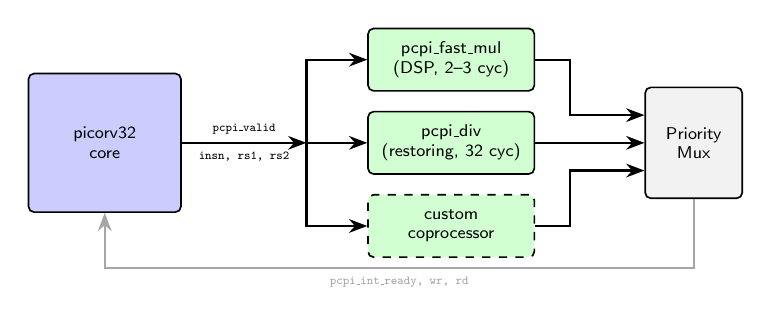
\begin{tikzpicture}[>=Stealth, semithick, scale=0.88, every node/.style={transform shape},
      blk/.style={draw, rounded corners=2pt, minimum height=0.9cm,
                  minimum width=2.4cm, font=\sffamily\scriptsize, align=center},
      arr/.style={->, thick},
      lbl/.style={font=\sffamily\tiny}]

    % CPU core
    \node[blk, fill=blue!20, minimum height=2.0cm, minimum width=2.2cm] (cpu) at (0, 0) {picorv32\\core};

    % PCPI port arrows (output) — fan-out point
    \draw[arr] (cpu.east) -- ++(1.8, 0) coordinate (fan)
      node[midway, above, lbl] {\texttt{pcpi\_valid}}
      node[midway, below, lbl] {\texttt{insn, rs1, rs2}};

    % Coprocessor modules — vertically centred on fan-out
    \node[blk, fill=green!18] (mul) at (5.0, 1.2) {pcpi\_fast\_mul\\(DSP, 2--3 cyc)};
    \node[blk, fill=green!18] (div) at (5.0, -0.0) {pcpi\_div\\(restoring, 32 cyc)};
    \node[blk, fill=green!18, dashed] (cust) at (5.0, -1.2) {custom\\coprocessor};

    \draw[arr] (fan) |- (mul.west);
    \draw[arr] (fan) -- (div.west);
    \draw[arr] (fan) |- (cust.west);

    % Priority mux — aligned with div (middle module)
    \node[blk, fill=gray!10, minimum width=1.4cm, minimum height=1.6cm] (mux) at (8.5, 0.0)
      {Priority\\Mux};

    \draw[arr] (mul.east) -- ++(0.5, 0) |- ([yshift=0.4cm]mux.west);
    \draw[arr] (div.east) -- (mux.west);
    \draw[arr] (cust.east) -- ++(0.5, 0) |- ([yshift=-0.4cm]mux.west);

    % Return path — clean horizontal below, then up into CPU
    \draw[arr, gray!70] (mux.south) -- ++(0, -1.0) -| (cpu.south)
      node[pos=0.25, below, lbl] {\texttt{pcpi\_int\_ready, wr, rd}};

    \end{tikzpicture}
    \caption{PCPI architecture. The CPU broadcasts \texttt{pcpi\_valid} with the instruction and operands to all connected coprocessors in parallel. Each coprocessor independently checks whether it handles the instruction. The priority mux combines their responses: the first to assert \texttt{ready} wins. On the iCEBreaker only \texttt{pcpi\_fast\_mul} and \texttt{pcpi\_div} are instantiated --- the custom slot (dashed) is unused.}
    \label{fig:pcpi-block}
\end{figure}

\paragraph{Built-in PCPI modules.} picorv32 ships with three optional coprocessors for the M~extension: \texttt{pcpi\_mul} (shift-and-add, $\sim$32 cycles, pure logic), \texttt{pcpi\_fast\_mul} (uses Verilog \texttt{*} operator $\to$ maps to iCE40 DSP blocks, 2--3 cycles), and \texttt{pcpi\_div} (restoring division, $\sim$32-cycle core / $\sim$40-cycle instruction). The iCEBreaker rv32im configuration enables \emph{both} \texttt{pcpi\_fast\_mul} (multiply) and \texttt{pcpi\_div} (divide), since \texttt{-march=rv32im} emits the full M-extension.

Table~\ref{tab:m-ext} lists the 8 M-extension instructions. All share the R-type opcode \texttt{0110011} with \texttt{funct7}=\texttt{0000001}. The base decoder (Table~\ref{tab:decode-unified}) does not recognise this funct7, so \texttt{instr\_trap} fires and the instruction is forwarded via PCPI. The multiply instructions differ only in which half of the 64-bit product they return: \texttt{mul} gives the lower 32~bits; \texttt{mulh}/\texttt{mulhsu}/\texttt{mulhu} give the upper 32~bits with different sign treatments. A full 64-bit product requires two instructions: \texttt{mulh~t1,~s3,~s5} then \texttt{mul~t2,~s3,~s5}, giving \texttt{\{t1,t2\} = s3 $\times$ s5}.

\begin{table}[htbp]
\centering\small
\renewcommand{\arraystretch}{1.15}
\begin{tabular*}{\textwidth}{@{\extracolsep{\fill}} l l l l l p{3.5cm} @{}}
    \toprule
    \texttt{funct3} & \texttt{funct7} & PCPI module & Asm & RTL & Description \\
    \midrule
    \texttt{000} & \texttt{0000001} & \texttt{pcpi\_fast\_mul} & \texttt{mul}    & \texttt{rd $\leftarrow$ (rs1$\times$rs2)[31:0]}   & Multiply (lower 32 bits) \\
    \texttt{001} & \texttt{0000001} & \texttt{pcpi\_fast\_mul} & \texttt{mulh}   & \texttt{rd $\leftarrow$ (rs1$\times$rs2)[63:32]}  & Multiply high (signed$\times$signed) \\
    \texttt{010} & \texttt{0000001} & \texttt{pcpi\_fast\_mul} & \texttt{mulhsu} & \texttt{rd $\leftarrow$ (rs1$\times$rs2)[63:32]}  & Multiply high (signed$\times$unsigned) \\
    \texttt{011} & \texttt{0000001} & \texttt{pcpi\_fast\_mul} & \texttt{mulhu}  & \texttt{rd $\leftarrow$ (rs1$\times$rs2)[63:32]}  & Multiply high (unsigned$\times$unsigned) \\
    \midrule
    \texttt{100} & \texttt{0000001} & \texttt{pcpi\_div}      & \texttt{div}    & \texttt{rd $\leftarrow$ rs1 / rs2}                & Divide (signed) \\
    \texttt{101} & \texttt{0000001} & \texttt{pcpi\_div}      & \texttt{divu}   & \texttt{rd $\leftarrow$ rs1 / rs2}                & Divide (unsigned) \\
    \texttt{110} & \texttt{0000001} & \texttt{pcpi\_div}      & \texttt{rem}    & \texttt{rd $\leftarrow$ rs1 \% rs2}               & Remainder (signed) \\
    \texttt{111} & \texttt{0000001} & \texttt{pcpi\_div}      & \texttt{remu}   & \texttt{rd $\leftarrow$ rs1 \% rs2}               & Remainder (unsigned) \\
    \bottomrule
\end{tabular*}
\caption{M-extension instructions handled via PCPI. All use R-type format with opcode \texttt{0110011} and \texttt{funct7}=\texttt{0000001}. On the iCEBreaker, \texttt{ENABLE\_FAST\_MUL}=1 maps multiply to DSP blocks (2--3 cycles) and \texttt{ENABLE\_DIV}=1 enables hardware division via \texttt{pcpi\_div} ($\sim$40-cycle instruction, $\sim$250 LUTs) --- required because \texttt{-march=rv32im} makes gcc emit \texttt{div}/\texttt{rem}.}
\label{tab:m-ext}
\end{table}

\clearpage

\subsection{Memory Interface}

The picorv32 uses a simple valid/ready handshake for \textbf{all memory access} --- instruction fetches, data loads, and data stores share a single bus. The CPU asserts \texttt{mem\_valid} with an address and (for writes) data; the memory system responds with \texttt{mem\_ready} and (for reads) data. A transaction completes on any rising clock edge where both \texttt{mem\_valid} and \texttt{mem\_ready} are high.

\paragraph{Three layers.} Before the wire-level detail, it helps to see the subsystem as \emph{three layers} (Figure~\ref{fig:mem-layers})

\begin{enumerate}
    \item \textbf{Internal bus layer} (Table~\ref{tab:mem-internal}). The CPU main FSM (\texttt{cpu\_state}, Figure~\ref{fig:picorv32-fsm}) never touches the external bus directly. It only raises one-cycle \emph{request} flags --- \texttt{mem\_do\_rinst} (fetch an instruction), \texttt{mem\_do\_rdata} (data load), \texttt{mem\_do\_wdata} (data store), \texttt{mem\_do\_prefetch} (speculative fetch) --- and later observes \texttt{mem\_done} (transaction finished) and \texttt{mem\_rdata\_q} (the latched read word). These wires never leave the core.
    \item \textbf{Bus FSM layer} (Table~\ref{tab:mem-fsm}, Figure~\ref{fig:mem-fsm}). A small 4-state controller (\texttt{mem\_state[1:0]}) sitting between the two buses: it consumes those internal requests, runs the valid/ready handshake on the external bus, and reports completion back to the CPU FSM. It is the \emph{only} block that drives the external bus.
    \item \textbf{External bus layer} (Table~\ref{tab:mem-signals}). The \texttt{mem\_*} wires (plus the one-cycle-early look-ahead \texttt{mem\_la\_*}) that cross the CPU\,$\leftrightarrow$\,memory boundary. PicoSoC's address decoder (Section~\ref{sec:picosoc}) routes them to flash, SPRAM, or a peripheral.
\end{enumerate}

Note that any component $\to$ \textit{drives} the next component on the right, which will reply with $\gets$ back to left component.

\begin{figure}[htbp]
    \centering
    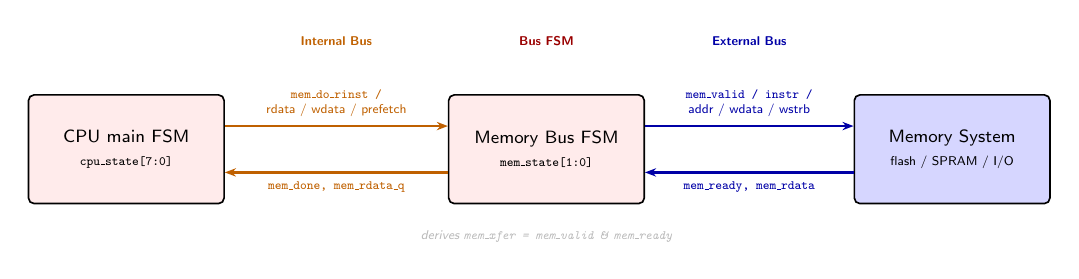
\begin{tikzpicture}[>=Stealth, semithick, scale=0.92, every node/.style={transform shape},
      box/.style={draw, rounded corners=2pt, minimum height=1.5cm, minimum width=2.7cm,
                  font=\sffamily\scriptsize, align=center},
      fsm/.style={box, fill=red!8},
      mem/.style={box, fill=blue!16},
      al/.style={font=\sffamily\tiny, align=center},
      req/.style={-{Stealth[length=4pt, width=3pt]}, thick, orange!75!black},
      bus/.style={-{Stealth[length=4pt, width=3pt]}, thick, blue!65!black}]

    \node[fsm] (cpu)    at (0, 0)    {CPU main FSM\\[1pt]{\ttfamily\tiny cpu\_state[7:0]}};
    \node[fsm] (busfsm) at (5.8, 0)  {Memory Bus FSM\\[1pt]{\ttfamily\tiny mem\_state[1:0]}};
    \node[mem] (m)      at (11.4, 0) {Memory System\\[1pt]{\tiny flash / SPRAM / I/O}};

    % Layer 1: CPU <-> bus FSM (internal requests / completion)
    \draw[req] ([yshift=0.32cm]cpu.east) -- ([yshift=0.32cm]busfsm.west)
      node[midway, above, al, text=orange!75!black]
      {\ttfamily mem\_do\_rinst /\\ rdata / wdata / prefetch};
    \draw[req] ([yshift=-0.32cm]busfsm.west) -- ([yshift=-0.32cm]cpu.east)
      node[midway, below, al, text=orange!75!black]
      {\ttfamily mem\_done, mem\_rdata\_q};

    % Layer 3: bus FSM <-> memory (external bus)
    \draw[bus] ([yshift=0.32cm]busfsm.east) -- ([yshift=0.32cm]m.west)
      node[midway, above, al, text=blue!65!black]
      {\ttfamily mem\_valid / instr /\\ addr / wdata / wstrb};
    \draw[bus] ([yshift=-0.32cm]m.west) -- ([yshift=-0.32cm]busfsm.east)
      node[midway, below, al, text=blue!65!black]
      {\ttfamily mem\_ready, mem\_rdata};

    % derived note under bus FSM (layer 2)
    \node[al, text=gray!55] at (5.8, -1.2)
      {\itshape derives \ttfamily mem\_xfer = mem\_valid \& mem\_ready};

    % region badges
    \node[al, text=orange!75!black] at (2.9, 1.5) {\bfseries Internal Bus};
    \node[al, text=red!60!black]    at (5.8, 1.5) {\bfseries Bus FSM};
    \node[al, text=blue!65!black]   at (8.6, 1.5) {\bfseries External Bus};

    \end{tikzpicture}
    \caption{The three layers of the picorv32 memory subsystem (detailed in the text), drawn left-to-right from core to memory: the \textbf{internal bus} (orange, the CPU FSM\,$\leftrightarrow$\,bus FSM request handshake), the \textbf{bus FSM} (red), and the \textbf{external bus} (blue, to flash/SPRAM/I/O via PicoSoC's decoder).}
    \label{fig:mem-layers}
\end{figure}

\subsubsection{Internal bus layer}

The CPU main FSM never drives the external bus directly; it talks to the bus FSM over a private handshake (Table~\ref{tab:mem-internal}) that never appears on a pin.

\begin{table}[htbp]
\centering\small
\begin{tabular}{@{}l c l p{6.3cm}@{}}
    \toprule
    Signal & Dir & Width & Function \\
    \midrule
    \texttt{mem\_do\_rinst}    & $\to$ & 1  & CPU FSM requests an instruction fetch \\
    \texttt{mem\_do\_rdata}    & $\to$ & 1  & CPU FSM requests a data load \\
    \texttt{mem\_do\_wdata}    & $\to$ & 1  & CPU FSM requests a data store \\
    \texttt{mem\_do\_prefetch} & $\to$ & 1  & CPU FSM requests a speculative (next-sequential) fetch \\
    \midrule
    \texttt{mem\_xfer}     & ---          & 1  & Derived as \texttt{mem\_valid \& mem\_ready}: a bus transfer completes this cycle \\
    \texttt{mem\_done}     & $\leftarrow$ & 1  & Bus FSM signals a fetch/load/store completed; releases the decoder (fetches) or \texttt{ldmem}/\texttt{stmem} (data) \\
    \texttt{mem\_rdata\_q} & $\leftarrow$ & 32 & Bus FSM's latched copy of \texttt{mem\_rdata}, held stable across CPU-FSM states \\
    \bottomrule
\end{tabular}
\caption{Internal bus signals --- the private handshake between the CPU main FSM (\texttt{cpu\_state}) and the bus FSM (\texttt{mem\_state}). Direction follows Figure~\ref{fig:mem-layers}: \texttt{$\to$} is CPU FSM\,$\to$\,bus FSM, \texttt{$\leftarrow$} is bus FSM\,$\to$\,CPU FSM. None of these appear on the external bus (contrast Table~\ref{tab:mem-signals}); \texttt{mem\_xfer} is not a stored signal but a combinational term used throughout the FSM.}
\label{tab:mem-internal}
\end{table}

The prefetch allows an extra fetch for free:

\begin{figure}[htbp]
    \centering
    \begin{tikztimingtable}[timing/wscale=2.2, timing/dslope=0.08,
      timing/d/background/.style={fill=blue!6}]
      \texttt{clk}               & 7{C}                                            \\
      \texttt{cpu\_state}        & 5D{CPU busy (current instr)} D{fetch} D{ld\_rs1} \\
      \texttt{mem\_do\_prefetch} & 5H 2L                                           \\
      \texttt{mem\_do\_rinst}    & 5L H L                                          \\
      \texttt{mem\_state}        & D{0} D{1} 4D{3 (parked)} D{0}                    \\
      \texttt{mem\_xfer}         & L H 5L                                          \\
      \texttt{mem\_done}         & 5L H L                                          \\
      \texttt{mem\_rdata\_q}     & 2Z {[timing/d/background/.style={fill=green!8}] 5D{instr word}} \\
    \end{tikztimingtable}
    \caption{Internal-bus timing for a \emph{prefetched} instruction fetch. While the CPU FSM is busy with a multi-cycle instruction it holds \texttt{mem\_do\_prefetch}, so the bus FSM fetches the \emph{next} instruction in the background: one bus transfer (\texttt{mem\_xfer}) latches the word into \texttt{mem\_rdata\_q} and the bus FSM \emph{parks} in state~3 \emph{without} firing \texttt{mem\_done}. The word then waits until the CPU finally reaches \texttt{fetch} and raises \texttt{mem\_do\_rinst}: the bus FSM returns state~3\,$\to$\,0 and fires \texttt{mem\_done} with \emph{no new bus transaction} --- the fetch is free. This is why a prefetch hides flash-fetch latency, and why state~1 routes a prefetch to state~3 rather than state~0 (Table~\ref{tab:mem-fsm} and its footnote).}
    \label{fig:mem-internal-timing}
\end{figure}

\clearpage
\subsubsection{Bus FSM layer}

The bus FSM is a 4-state machine \texttt{mem\_state[1:0]} that runs in parallel with the CPU FSM: it consumes the internal \texttt{mem\_do\_*} requests and drives the external bus. Table~\ref{tab:mem-fsm} details the states; Figure~\ref{fig:mem-fsm} shows the transitions.

\begin{table}[htbp]
\centering\small
\renewcommand{\arraystretch}{1.25}
\begin{tabular}{@{}c l p{8.5cm}@{}}
    \toprule
    State & Name & Description \\
    \midrule
    0 & Idle & No transaction in progress. If \texttt{mem\_do\_rinst}, \texttt{mem\_do\_rdata}, or \texttt{mem\_do\_prefetch} is asserted, asserts \texttt{mem\_valid} (unless using a prefetched high word) and transitions to state~1. If \texttt{mem\_do\_wdata}, asserts \texttt{mem\_valid} with write strobes and transitions to state~2. \\
    1 & Read pending & Waiting for \texttt{mem\_ready}. On \texttt{mem\_xfer} (= \texttt{mem\_valid \& mem\_ready}), latches read data into \texttt{mem\_rdata\_q}. If this was an instruction fetch or data read, returns to state~0; if a prefetch, transitions to state~3.\footnotemark{} \\
    2 & Write pending & Waiting for \texttt{mem\_ready} with write strobes active. On \texttt{mem\_xfer}, deasserts \texttt{mem\_valid} and returns to state~0. \\
    3 & Prefetch done & Holds the speculatively fetched instruction. When the CPU FSM later requests an instruction read (\texttt{mem\_do\_rinst}), the prefetched data is already available and the FSM returns to state~0 without issuing a new bus transaction. \\
    \bottomrule
\end{tabular}
\caption{Memory bus FSM states (\texttt{mem\_state[1:0]}). The \texttt{mem\_done} signal fires when a read or write completes (state 1$\to$0 or 2$\to$0), triggering the instruction decoder (for fetches) or allowing \texttt{ldmem}/\texttt{stmem} to proceed.}
\label{tab:mem-fsm}
\end{table}
\footnotetext{The bus FSM does not itself remember the request type; at \texttt{mem\_xfer} it re-reads the CPU FSM's still-asserted request flags --- \texttt{mem\_state <= mem\_do\_rinst || mem\_do\_rdata ? 0 : 3} (\texttt{picorv32.v} line~617). Those flags are held for the whole transaction (cleared only by \texttt{mem\_done}), so \texttt{mem\_do\_prefetch} alone --- a speculative fetch the CPU is not yet waiting on --- routes to state~3, whereas \texttt{mem\_do\_rinst}/\texttt{mem\_do\_rdata} (the CPU is stalled now) route back to state~0. Note \texttt{mem\_instr} cannot make this distinction: it is~1 for both \texttt{prefetch} and \texttt{rinst}.}

\begin{figure}[htbp]
    \centering
    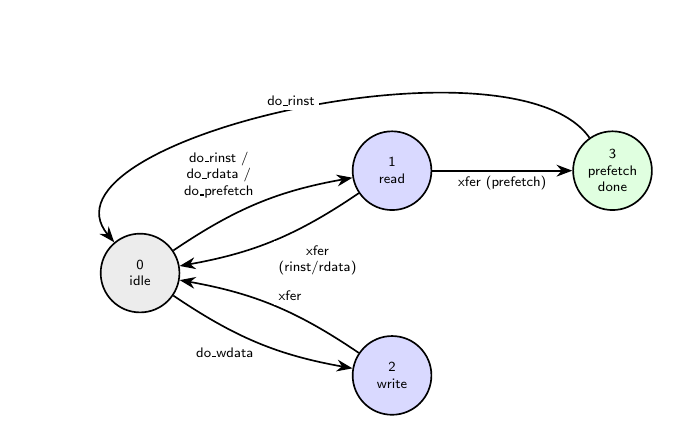
\begin{tikzpicture}[>=Stealth, semithick,
      st/.style={draw, circle, minimum size=1.0cm,
                 font=\sffamily\tiny, inner sep=1pt, align=center},
      lbl/.style={font=\sffamily\tiny, inner sep=1.5pt, fill=white, align=center}]

    % Compact layout: idle left; read top / write bottom; prefetch-done top-right.
    \node[st, fill=gray!15]  (s0) at (0, 0)      {0\\idle};
    \node[st, fill=blue!15]  (s1) at (3.2, 1.3)  {1\\read};
    \node[st, fill=blue!15]  (s2) at (3.2, -1.3) {2\\write};
    \node[st, fill=green!12] (s3) at (6.0, 1.3)  {3\\prefetch\\done};

    % Idle <-> Read : two arcs bowing to opposite sides
    \draw[->] (s0) to[bend left=12]
        node[lbl, above left] {do\_rinst /\\do\_rdata /\\do\_prefetch} (s1);
    \draw[->] (s1) to[bend left=12]
        node[lbl, below right] {xfer\\(rinst/rdata)} (s0);

    % Idle <-> Write : mirror below
    \draw[->] (s0) to[bend right=12]
        node[lbl, below left] {do\_wdata} (s2);
    \draw[->] (s2) to[bend right=12]
        node[lbl, above right] {xfer} (s0);

    % Read -> Prefetch done
    \draw[->] (s1) -- node[lbl, below] {xfer (prefetch)} (s3);

    % Prefetch done -> Idle : shorter, flatter arc over the top
    \draw[->] (s3) to[out=125, in=130, looseness=0.7]
        node[lbl, above, pos=0.5] {do\_rinst} (s0);

    \end{tikzpicture}
    \caption{Memory bus FSM. The idle state dispatches to read (state~1) or write (state~2) based on CPU request signals. Reads complete back to idle; prefetches park in state~3 until the CPU needs the instruction. An instruction cache does \emph{not} change this FSM: it sits one layer out as a PicoSoC bus responder (selected by address, \S\ref{sec:picosoc}), so the bus FSM still issues \texttt{mem\_valid} and parks in state~1 --- the cache merely returns \texttt{mem\_ready} in ${\sim}2$ cycles on a hit instead of the ${\sim}128$ a flash read costs.}
    \label{fig:mem-fsm}
\end{figure}

\subsubsection{External bus layer}

Finally, Table~\ref{tab:mem-signals} lists the wires that actually cross the CPU\,$\leftrightarrow$\,memory boundary --- the only layer the memory system sees. All CPU outputs are registered; inputs are sampled combinationally. The instruction cache lives at \emph{this} layer: it is one of PicoSoC's external-bus responders (\S\ref{sec:picosoc}), answering \texttt{mem\_ready}/\texttt{mem\_rdata} for the flash address range, transparently to the CPU and bus FSM above.

\begin{table}[htbp]
\centering\small
\begin{tabular}{@{}l c l p{6.3cm}@{}}
    \toprule
    Signal & Dir & Width & Function \\
    \midrule
    \texttt{mem\_valid} & $\to$ & 1 & CPU asserts to request a transaction \\
    \texttt{mem\_instr} & $\to$ & 1 & 1 = instruction fetch, 0 = data access \\
    \texttt{mem\_addr} & $\to$ & 32 & Byte address (word-aligned for 32-bit access) \\
    \texttt{mem\_wdata} & $\to$ & 32 & Write data (valid when \texttt{mem\_wstrb} $\neq$ 0) \\
    \texttt{mem\_wstrb} & $\to$ & 4 & Any 1 bit indicates write byte-enables; \texttt{0000} = read \\
    \texttt{mem\_ready} & $\leftarrow$ & 1 & Memory asserts to complete the transaction \\
    \texttt{mem\_rdata} & $\leftarrow$ & 32 & Read data (valid when \texttt{mem\_ready} \& \texttt{wstrb}=0) \\
    \midrule
    \texttt{mem\_la\_read} & $\to$ & 1 & Look-ahead: read will be requested next cycle \\
    \texttt{mem\_la\_write} & $\to$ & 1 & Look-ahead: write will be requested next cycle \\
    \texttt{mem\_la\_addr} & $\to$ & 32 & Look-ahead address (available one cycle early) \\
    \texttt{mem\_la\_wdata} & $\to$ & 32 & Look-ahead write data \\
    \texttt{mem\_la\_wstrb} & $\to$ & 4 & Look-ahead write strobes \\
    \bottomrule
\end{tabular}
\caption{picorv32 external memory-interface signals. The upper group is the primary valid/ready handshake; the lower group is the look-ahead interface that presents each transaction one cycle early. The \texttt{$\to$}/\texttt{$\leftarrow$} direction convention is defined in Figure~\ref{fig:mem-layers} (\texttt{$\to$} = CPU\,$\to$\,memory, \texttt{$\leftarrow$} = memory\,$\to$\,CPU).}
\label{tab:mem-signals}
\end{table}

\texttt{mem\_instr} lets the memory system route instruction fetches to SPI flash and data accesses to SPRAM. \texttt{mem\_wstrb} = \texttt{0000} signals a read; any non-zero pattern is a write with byte-granularity enables.

\paragraph{Look-ahead interface.} Synchronous memories (EBR, SPRAM) need the address one clock cycle before the data is available. The look-ahead signals (\texttt{mem\_la\_*}) provide the address, data, and strobes \textbf{one cycle before} \texttt{mem\_valid}, so the memory can begin its internal access immediately and have the result ready when \texttt{mem\_valid} goes high.\footnote{PicoSoC does not actually route the look-ahead bus (the \texttt{cpu} instance in \texttt{picosoc.v} wires only \texttt{mem\_valid/instr/ready/addr/wdata/wstrb/rdata}); its SPRAM instead uses a registered \texttt{ram\_ready} pulse, so a data access completes the cycle \emph{after} \texttt{mem\_valid} (one wait state) rather than the same cycle shown in Figure~\ref{fig:mem-timing}. That same-cycle response is the core interface's look-ahead \emph{capability}, not what this SoC wires up.} Figure~\ref{fig:mem-timing} shows the timing.\footnote{How to read the waveforms: a single-bit signal (e.g.\ \texttt{mem\_valid}) is one line that toggles high/low. A multi-bit bus (e.g.\ \texttt{mem\_addr}, \texttt{mem\_rdata}) is drawn as a flat line while it carries no meaningful value (idle/don't-care), and \emph{opens into a labelled band} only while it holds a valid value.}

\begin{figure}[htbp]
    \centering
    \begin{minipage}[t]{0.49\textwidth}
      \centering
      \textbf{\small (a) Load}\par\smallskip
      \begin{tikztimingtable}[timing/wscale=3, timing/dslope=0.08,
        timing/d/background/.style={fill=blue!6}]
        \texttt{clk}           & 5{C}          \\
        \texttt{mem\_la\_read} & L H 3L        \\
        \texttt{mem\_la\_addr} & Z D{addr} 3Z  \\
        \texttt{mem\_valid}    & 2L H 2L       \\
        \texttt{mem\_instr}    & 5L            \\
        \texttt{mem\_addr}     & 2Z D{addr} 2Z \\
        \texttt{mem\_wstrb}    & 2Z D{0000} 2Z \\
        \texttt{mem\_ready}    & 2L H 2L       \\
        \texttt{mem\_rdata}    & 2Z D{data} 2Z \\
      \end{tikztimingtable}
    \end{minipage}\hfill
    \begin{minipage}[t]{0.49\textwidth}
      \centering
      \textbf{\small (b) Store}\par\smallskip
      \begin{tikztimingtable}[timing/wscale=3, timing/dslope=0.08,
        timing/d/background/.style={fill=blue!8}]
        \texttt{clk}            & 5{C}          \\
        \texttt{mem\_la\_write} & L H 3L        \\
        \texttt{mem\_la\_addr}  & Z D{addr} 3Z  \\
        \texttt{mem\_la\_wdata} & Z D{data} 3Z  \\
        \texttt{mem\_la\_wstrb} & Z D{1111} 3Z  \\
        \texttt{mem\_valid}     & 2L H 2L       \\
        \texttt{mem\_instr}     & 5L            \\
        \texttt{mem\_addr}      & 2Z D{addr} 2Z \\
        \texttt{mem\_wdata}     & 2Z D{data} 2Z \\
        \texttt{mem\_wstrb}     & 2Z D{1111} 2Z \\
        \texttt{mem\_ready}     & 2L H 2L       \\
      \end{tikztimingtable}
    \end{minipage}
    \caption{Memory bus timing for (a) a load and (b) a store, drawn with the look-ahead interface. The \texttt{mem\_la\_*} signals present the address (and, for a store, the write data and strobes) \textbf{one cycle before} \texttt{mem\_valid}, giving synchronous memory (EBR/SPRAM) a cycle to register the address. \texttt{mem\_instr}=0 in both, since these are data accesses (an instruction fetch would assert it); \texttt{mem\_wstrb}=\texttt{0000} marks the load as a read, \texttt{1111} a full-word store. These are \emph{data} accesses, which in PicoSoC target single-cycle SPRAM; \emph{instruction} fetches instead go to SPI flash and stall for many wait states (Figure~\ref{fig:mem-timing-flash}). Here the memory responds immediately (\texttt{mem\_ready} in the same cycle as \texttt{mem\_valid}), so each transaction completes in one \texttt{mem\_valid} cycle; a slower memory holds \texttt{mem\_ready} low to insert wait states.}
    \label{fig:mem-timing}
\end{figure}

By contrast, an instruction fetch targets SPI flash, and \texttt{spimemio} holds \texttt{mem\_ready} low for many cycles (while \texttt{spimemio} is reading).

\begin{figure}[htbp]
    \centering
    \begin{tikztimingtable}[timing/wscale=3, timing/dslope=0.08,
      timing/d/background/.style={fill=blue!6}]
      \texttt{clk}           & 8{C}                       \\
      \texttt{mem\_la\_read} & L H 6L                     \\
      \texttt{mem\_la\_addr} & Z D{addr} 6Z               \\
      \texttt{mem\_valid}    & 2L 5H L                    \\
      \texttt{mem\_instr}    & 2L 5H L                    \\
      \texttt{mem\_addr}     & 2Z 5D{flash addr (held)} Z \\
      \texttt{mem\_wstrb}    & 2Z 5D{0000} Z              \\
      \texttt{mem\_ready}    & 6L H L                     \\
      \texttt{mem\_rdata}    & 6Z D{instr} Z \\
    \end{tikztimingtable}
    \caption{Instruction fetch from SPI flash --- the slow path. \texttt{mem\_instr}=1 routes the request to \texttt{spimemio}; \texttt{mem\_wstrb}=\texttt{0000} marks it a read. Unlike the single-cycle SPRAM accesses of Figure~\ref{fig:mem-timing}, the flash controller holds \texttt{mem\_ready} \emph{low} for many SPI cycles, while \texttt{mem\_valid}/\texttt{mem\_addr} stay asserted; \texttt{mem\_rdata} returns only on the final cycle. The wait window here is compressed --- a real single-bit fetch is $\sim$64 SPI clocks $\approx$ 128 system cycles at the 2:1 SCK divider (\S\ref{sec:spimemio}).}
    \label{fig:mem-timing-flash}
\end{figure}

\newpage
\subsection{SPI Flash Controller (\texttt{spimemio})}
\label{sec:spimemio}

\texttt{spimemio} serves instruction fetch requests from the CPU (specifically memory bus FSM) and exposes a config register at \texttt{0x02000000}. It has \emph{no cache} --- it \emph{streams} sequential reads, advancing word by word. Since all code runs in place from flash (Section~\ref{sec:picosoc}), it sets the fetch latency that dominates the baseline (Section~\ref{sec:optspace}).

\paragraph{Transaction structure.} A read is a fixed sequence of phases driven by a 13-state FSM (Table~\ref{tab:spimemio-phases}, Figure~\ref{fig:spimemio-fsm}); the inner \texttt{spimemio\_xfer} engine shifts each byte over the flash pins at SCK = half the system clock rate. Single-bit SPI shifts 1 bit per SCK, while Dual-/Quad-I/O shift 2/4 bits --- using less number of SPI cycles (Figure~\ref{fig:spi-timing}). These are all \emph{single-data-rate} (SDR): one transfer per rising SCK edge, so the lane count (1/2/4) sets the bits per clock. \emph{Double-data-rate} (DDR) clocks data on \emph{both} the rising and falling edges of SCK, doubling the bits-per-clock again, so quad-DDR (\texttt{0xED}) moves 8 bits per SCK, twice quad-SDR. The price is tighter I/O timing, since the controller must drive and sample data on both edges (the negedge-registered \texttt{xfer\_io*\_90} path in \texttt{spimemio\_xfer}).

\begin{table}[htbp]
\centering\small
\renewcommand{\arraystretch}{1.2}
\begin{tabular}{@{}c l p{8.7cm}@{}}
    \toprule
    State & Phase & Action \\
    \midrule
    0--1  & Power-up & Send \texttt{0xFF} (terminate any continuous-read mode), then wait. \\
    2--3  & Wake     & Send \texttt{0xAB} (release power-down), then wait. \\
    4     & Command  & Issue the SPI read opcode --- \texttt{0x03} (single), \texttt{0xBB} (dual), \texttt{0xEB} (quad), or \texttt{0xED} (quad DDR) --- selected by \{\texttt{config\_ddr}, \texttt{config\_qspi}\}. \\
    5--7  & Address  & Shift 3$\times$ byte address (\texttt{addr[23:16]}, \texttt{[15:8]}, \texttt{[7:0]}) for 24 bits\\
    8     & Mode\,+\,dummy & (QSPI/DDR only) send the continuation byte (\texttt{0xA5} if \texttt{config\_cont}, else \texttt{0xFF}) followed by \texttt{config\_dummy} dummy cycles. \\
    9--12 & Data     & Read 4 bytes into the 32-bit word. State~12 loops back to~9 for the next sequential word, keeping the command open. \\
    \bottomrule
\end{tabular}
\caption{\texttt{spimemio} read-transaction phases (FSM \texttt{state[3:0]}). States 0--3 run once after reset, while states 4--12 form each read. For streaming sequential words, states 9--12 loop over itself.}
\label{tab:spimemio-phases}
\end{table}

\begin{figure}[htbp]
    \centering
    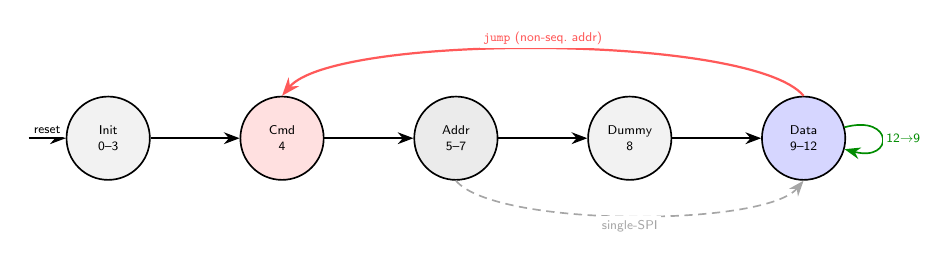
\begin{tikzpicture}[>=Stealth, semithick, scale=0.92, every node/.style={transform shape},
      st/.style={draw, circle, minimum size=1.15cm, font=\sffamily\tiny, inner sep=0.5pt, align=center},
      lbl/.style={font=\sffamily\tiny, inner sep=1.5pt, fill=white, align=center}]

    \node[st, fill=gray!10] (init) at (0, 0)   {Init\\0--3};
    \node[st, fill=red!12]  (cmd)  at (2.4, 0)  {Cmd\\4};
    \node[st, fill=gray!16] (addr) at (4.8, 0)  {Addr\\5--7};
    \node[st, fill=gray!10] (dum)  at (7.2, 0)  {Dummy\\8};
    \node[st, fill=blue!16] (data) at (9.6, 0)  {Data\\9--12};

    \draw[->] (-1.1, 0) -- (init) node[midway, above, lbl] {reset};
    \draw[->] (init) -- (cmd);
    \draw[->] (cmd)  -- (addr);
    \draw[->] (addr) -- (dum);
    \draw[->] (dum)  -- (data);

    % single-SPI skips the mode/dummy state (7 -> 9)
    \draw[->, densely dashed, gray!70] (addr.south) to[out=-50, in=-130, looseness=0.45]
        node[pos=0.5, below, lbl, text=gray!70] {single-SPI} (data.south);

    % streaming: keep command open, advance rd_addr by 4 (12 -> 9)
    \path (data) edge[->, green!55!black, loop right, looseness=6]
        node[right, lbl, text=green!55!black] {12$\to$9} (data);

    % jump: non-sequential address restarts the burst
    \draw[->, red!65, thick] (data.north) to[out=130, in=50, looseness=0.4]
        node[pos=0.5, above, lbl, text=red!65] {\texttt{jump} (non-seq.\ addr)} (cmd.north);

    \end{tikzpicture}
    \caption{\texttt{spimemio} read FSM, grouped by phase (state numbers from Table~\ref{tab:spimemio-phases}). States 0--3 run once after reset; each read then walks Cmd\,$\to$\,Addr\,$\to$\,Dummy\,$\to$\,Data, and single-bit SPI skips the mode/dummy state (\textcolor{gray}{dashed}, $7\to9$). \textcolor{green!55!black}{Green}: sequential streaming --- the Data phase loops ($12\to9$), advancing \texttt{rd\_addr} by~4 and keeping the flash command open, so consecutive words cost only their data phase. \textcolor{red!65}{Red}: a \texttt{jump} (non-sequential fetch) aborts the burst and re-issues the command and address --- the per-branch penalty that a cache or line buffer removes (Section~\ref{sec:fastflash}).}
    \label{fig:spimemio-fsm}
\end{figure}

Figure~\ref{fig:spi-timing} gives the per-word cost: $\sim$64 SPI clocks for single-SPI, $\sim$20 SCK clocks for Quad-I/O$+$CRM, while sustained sequential reads take $\sim$8 SCK clocks. \footnote{$\sim$128, $\sim$40, and $\sim$16 \emph{system} cycles at the 2:1 SCK divider}

\begin{figure}[htbp]
    \centering
    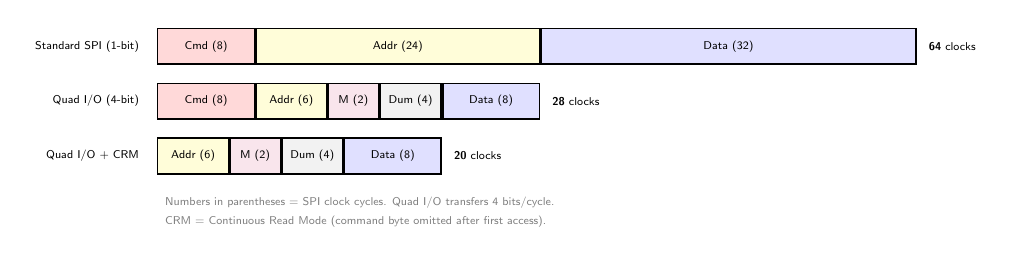
\begin{tikzpicture}[>=Stealth, semithick, scale=0.82, every node/.style={transform shape},
      phase/.style={draw, minimum height=0.55cm, inner sep=1pt,
                    font=\sffamily\tiny, align=center},
      lbl/.style={font=\sffamily\tiny}]

    \def\ox{2.2}   % left edge of all phase bars (after labels)
    \def\rh{0.85}  % row spacing
    % Semi-proportional widths: bp * clocks, with a floor so text fits
    % bp=0.14 gives good proportions; floor of 0.55cm for 2-clock phases
    \def\bp{0.14}
    \newcommand{\pw}[1]{\pgfmathmax(#1*\bp, 0.55)\pgfmathresult}

    % Row labels (right-aligned at consistent x)
    \node[lbl, anchor=east] at (\ox-0.15, 0)      {Standard SPI (1-bit)};
    \node[lbl, anchor=east] at (\ox-0.15, -\rh)   {Quad I/O (4-bit)};
    \node[lbl, anchor=east] at (\ox-0.15, -2*\rh) {Quad I/O + CRM};

    % Standard SPI: Cmd(8) + Addr(24) + Data(32) = 64 (0x03 read has no dummy phase)
    \node[phase, fill=red!15,    minimum width=1.5cm, anchor=west] (s1) at (\ox, 0) {Cmd (8)};
    \node[phase, fill=yellow!15, minimum width=4.4cm, anchor=west] (s2) at (s1.east) {Addr (24)};
    \node[phase, fill=blue!12,   minimum width=5.8cm, anchor=west] (s4) at (s2.east) {Data (32)};
    \node[lbl, anchor=west] at (s4.east) {~\textbf{64} clocks};

    % Quad SPI: Cmd(8, single-lane) + Addr(6) + M(2) + Dum(4) + Data(8) = 28
    \node[phase, fill=red!15,    minimum width=1.5cm, anchor=west] (q1) at (\ox, -\rh) {Cmd (8)};
    \node[phase, fill=yellow!15, minimum width=1.1cm, anchor=west] (q2) at (q1.east) {Addr (6)};
    \node[phase, fill=purple!10, minimum width=0.78cm, anchor=west] (q3) at (q2.east) {M (2)};
    \node[phase, fill=gray!10,   minimum width=0.95cm, anchor=west] (q4) at (q3.east) {Dum (4)};
    \node[phase, fill=blue!12,   minimum width=1.5cm, anchor=west] (q5) at (q4.east) {Data (8)};
    \node[lbl, anchor=west] at (q5.east) {~\textbf{28} clocks};

    % QSPI + CRM: Addr(6) + M(2) + Dum(4) + Data(8) = 20  (no Cmd)
    \node[phase, fill=yellow!15, minimum width=1.1cm, anchor=west] (c1) at (\ox, -2*\rh) {Addr (6)};
    \node[phase, fill=purple!10, minimum width=0.78cm, anchor=west] (c2) at (c1.east) {M (2)};
    \node[phase, fill=gray!10,   minimum width=0.95cm, anchor=west] (c3) at (c2.east) {Dum (4)};
    \node[phase, fill=blue!12,   minimum width=1.5cm, anchor=west] (c4) at (c3.east) {Data (8)};
    \node[lbl, anchor=west] at (c4.east) {~\textbf{20} clocks};

    % Annotation
    \node[font=\sffamily\tiny, text=gray, anchor=north west] at (\ox, -2*\rh-0.5)
      {Numbers in parentheses = SPI clock cycles. Quad I/O transfers 4 bits/cycle.};
    \node[font=\sffamily\tiny, text=gray, anchor=north west] at (\ox, -2*\rh-0.8)
      {CRM = Continuous Read Mode (command byte omitted after first access).};

    \end{tikzpicture}
    \caption{SPI flash read transaction overhead for one 32-bit word. Standard SPI transmits 1 bit per clock: 8 (command) + 24 (address) + 32 (data) = 64 SPI clocks (the \texttt{0x03} read has no dummy phase). Quad I/O sends the command single-lane (8 clocks) but transfers address and data 4 bits per clock, reducing the total to $\sim$28 SPI clocks. CRM omits the command byte on later accesses, cutting this to $\sim$20. The \texttt{spimemio} controller keeps the flash command open and streams sequential words, so sustained throughput in QSPI+CRM drops to $\sim$8 SPI clocks per word (data phase only).}
    \label{fig:spi-timing}
\end{figure}

\pagebreak
\paragraph{Configuration register.} The mode is held in \texttt{cfgreg} (Table~\ref{tab:spimemio-cfgreg}), writable at \texttt{0x02000000}. \texttt{config\_en}=1 lets the controller drive the flash automatically; \texttt{config\_en}=0 hands the pins to firmware for manual bit-banging --- used by \texttt{flashio\_worker} in \texttt{start.s} to program the chip's status registers (e.g.\ setting the QE bit). The remaining fields select the read command, dummy-cycle count, and continuous-read mode.

\begin{table}[htbp]
\centering\small
\begin{tabular}{@{}l l l@{}}
    \toprule
    Bit(s) & Field & Meaning \\
    \midrule
    \texttt{[31]}    & \texttt{config\_en}       & MEMIO enable (reset 1; 0 = manual bit-bang) \\
    \texttt{[22]}    & \texttt{config\_ddr}      & DDR enable (reset 0) \\
    \texttt{[21]}    & \texttt{config\_qspi}     & Quad-I/O enable (reset 0) \\
    \texttt{[20]}    & \texttt{config\_cont}     & CRM / continuous-read enable (reset 0) \\
    \texttt{[19:16]} & \texttt{config\_dummy}    & dummy cycles after address (reset: 8) \\
    \texttt{[11:8]}  & \texttt{config\_oe}       & manual output-enables (\texttt{config\_en}=0 only) \\
    \texttt{[5:4]}   & \texttt{config\_csb/clk}  & manual CSB / SCK (\texttt{config\_en}=0 only) \\
    \texttt{[3:0]}   & \texttt{config\_do}       & manual data-out pins (\texttt{config\_en}=0 only) \\
    \bottomrule
\end{tabular}
\caption{\texttt{spimemio} \texttt{cfgreg} (\texttt{0x02000000}), after the upstream picosoc map. Bits \texttt{[22:20]} jointly select the read command: \{\texttt{config\_ddr},\texttt{config\_qspi}\} decodes as \texttt{00}$\to$\texttt{0x03} single-bit, \texttt{10}$\to$\texttt{0xBB} Dual I/O (single-rate), \texttt{01}$\to$\texttt{0xEB} Quad I/O, \texttt{11}$\to$\texttt{0xED} DDR Quad I/O --- so \texttt{config\_ddr} alone (with \texttt{config\_qspi}=0) selects \emph{dual}, not double-data-rate. \texttt{config\_cont} (CRM) then drops the command byte on subsequent reads, sending mode byte \texttt{0xA5} instead of \texttt{0xFF}. All read-mode bits reset to 0, so the controller powers up in the slowest single-SPI \texttt{0x03} mode (\S\ref{sec:fastflash}); \texttt{config\_dummy} resets to 8 but only applies to the QSPI/DDR commands. The lower fields (\texttt{[11:8]}, \texttt{[5:4]}, \texttt{[3:0]}) are the manual bit-bang interface, active only when \texttt{config\_en}=0 --- used at boot by \texttt{flashio\_worker} to set the flash chip's QE bit.}
\label{tab:spimemio-cfgreg}
\end{table}

\paragraph{Sequential streaming and the jump penalty.} A fetch hits immediately when its address matches the streamer's running address; the controller then advances by one word and keeps the flash command open ($12\to9$), so consecutive words cost only their data phase. But any \emph{non-sequential} address raises \texttt{jump}, aborting the burst and restarting at the command/address phase. Every taken branch, call, and return therefore pays the full command$+$address$+$dummy latency --- the motivation for the line buffer in Section~\ref{sec:fastflash}.

\paragraph{Reset defaults.} On reset the controller comes up in its slowest mode --- standard single-bit SPI (the \texttt{0x03} read, $\sim$64 SPI clocks/word) --- and nothing switches it faster unless firmware writes \texttt{cfgreg}. Changing these reset values is the cheapest fetch-latency win (Section~\ref{sec:fastflash}).

\newpage
\subsection{PicoSoC}
\label{sec:picosoc}

PicoSoC is a minimal system-on-chip wrapper that connects the picorv32 CPU to 3 physical memories and peripherals with no bus fabric --- just combinational address decode logic.

\subsubsection{Physical Memories}

\paragraph{SPRAM (128\,KB)} Main data memory.\footnote{In the default PicoSoC, a small EBR-backed RAM (\texttt{picosoc\_mem}, 256 words = 1\,KB) serves as data memory (stack, locals). However on the iCEBreaker, \texttt{icebreaker.v} overrides this with SPRAM (\texttt{PICOSOC\_MEM = ice40up5k\_spram}), so \textit{no EBR is used for main memory}.} SPRAM is hard configured physically to have only 16-bit data width, is \emph{not pre-loadable} and is \emph{single-port} --- only one read or write per cycle. Hence to achieve 32-bit width, four \texttt{SB\_SPRAM256KA} blocks wired as shown in Figure~\ref{fig:spram-wiring}: two banks, each composed of two blocks side-by-side (one for \texttt{wdata[15:0]}, the other for \texttt{wdata[31:16]}), giving 32-bit width per bank. \texttt{addr[14]} selects between the two 64\,KB banks via \texttt{CHIPSELECT}; \texttt{addr[13:0]} addresses within a bank.\footnote{\texttt{addr} is the wrapper's local port name (\texttt{input [21:0] addr}); \texttt{picosoc.v} drives it with \texttt{mem\_addr[23:2]}, of which only \texttt{addr[14:0]} carry information --- see the address-width note after Table~\ref{tab:picosoc-addrmap}.}

\begin{figure}[htbp]
    \centering
    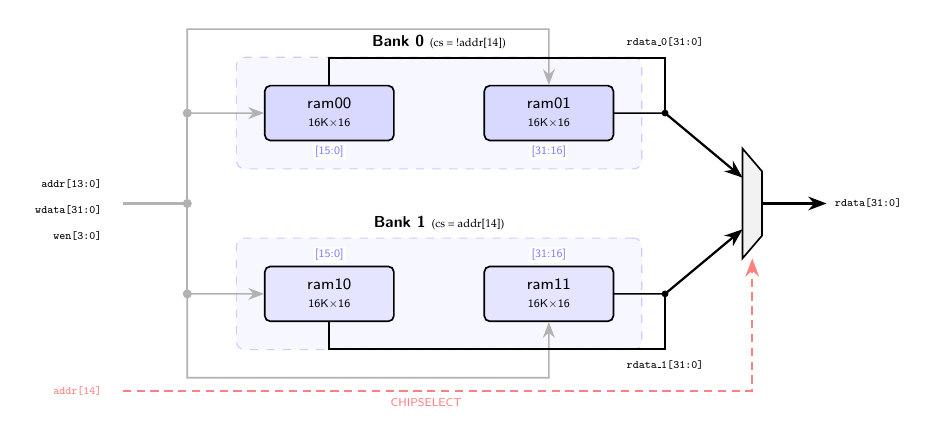
\begin{tikzpicture}[>=Stealth, semithick, scale=0.82, every node/.style={transform shape},
      blk/.style={draw, rounded corners=2pt, minimum height=0.85cm,
                  minimum width=2.0cm, font=\sffamily\scriptsize, align=center},
      arr/.style={->, thick},
      lbl/.style={font=\sffamily\tiny},
      flbl/.style={font=\sffamily\tiny, fill=white, inner sep=1pt}]

    % ---- Layout ----
    \def\by{1.4}       % Bank 0 y
    \def\bylo{-1.4}    % Bank 1 y
    \def\bL{2.0}       % left block x
    \def\bR{5.4}       % right block x

    % ---- RAM blocks ----
    \node[blk, fill=blue!15] (r00) at (\bL, \by)   {ram00\\{\tiny 16K$\times$16}};
    \node[blk, fill=blue!15] (r01) at (\bR, \by)   {ram01\\{\tiny 16K$\times$16}};
    \node[blk, fill=blue!10] (r10) at (\bL, \bylo)  {ram10\\{\tiny 16K$\times$16}};
    \node[blk, fill=blue!10] (r11) at (\bR, \bylo)  {ram11\\{\tiny 16K$\times$16}};

    % ---- Bank boxes ----
    \begin{scope}[on background layer]
    \node[draw=blue!20, dashed, rounded corners=3pt, inner sep=10pt, fill=blue!3,
          fit=(r00)(r01), label={[font=\sffamily\scriptsize\bfseries]above:Bank 0 \normalfont\tiny(cs = !addr[14])}] {};
    \node[draw=blue!20, dashed, rounded corners=3pt, inner sep=10pt, fill=blue!3,
          fit=(r10)(r11), label={[font=\sffamily\scriptsize\bfseries]above:Bank 1 \normalfont\tiny(cs = addr[14])}] {};
    \end{scope}

    % ---- Input bus: single bus line from left, forking to each block ----
    % One horizontal bus at y=0 (between banks), then vertical branches up/down
    \coordinate (bus) at (-1.2, 0);

    % Bus label block
    \node[lbl, anchor=east, align=right] at (-1.4, 0.3)  {\texttt{addr[13:0]}};
    \node[lbl, anchor=east, align=right] at (-1.4, -0.1) {\texttt{wdata[31:0]}};
    \node[lbl, anchor=east, align=right] at (-1.4, -0.5) {\texttt{wen[3:0]}};

    % Horizontal bus line
    \def\tx{-0.2}  % trunk x (well left of blocks)
    \draw[thick, gray!60] (bus) -- (\tx, 0);
    \fill[gray!60] (\tx, 0) circle (2pt);

    % Upward to Bank 0: left block gets a direct horizontal arrow
    \draw[thick, gray!60] (\tx, 0) -- (\tx, \by);
    \fill[gray!60] (\tx, \by) circle (2pt);
    \draw[->, gray!60] (\tx, \by) -- (r00.west);
    % Right block: UP to clearance, flat RIGHT to above r01, then DOWN into r01.north
    \pgfmathsetmacro{\byroute}{\by + 1.3}
    \draw[->, gray!60] (\tx, \by) -- (\tx, \byroute) -- (\bR, \byroute) -- (r01.north);

    % Downward to Bank 1: mirror pattern
    \draw[thick, gray!60] (\tx, 0) -- (\tx, \bylo);
    \fill[gray!60] (\tx, \bylo) circle (2pt);
    \draw[->, gray!60] (\tx, \bylo) -- (r10.west);
    % Right block: DOWN to clearance, flat RIGHT to below r11, then UP into r11.south
    \pgfmathsetmacro{\byloroute}{\bylo - 1.3}
    \draw[->, gray!60] (\tx, \bylo) -- (\tx, \byloroute) -- (\bR, \byloroute) -- (r11.south);

    % Bit-slice annotations next to each block
    \node[flbl, text=blue!50] at (\bL, \by-0.6)   {\tiny [15:0]};
    \node[flbl, text=blue!50] at (\bR, \by-0.6)   {\tiny [31:16]};
    \node[flbl, text=blue!50] at (\bL, \bylo+0.6)  {\tiny [15:0]};
    \node[flbl, text=blue!50] at (\bR, \bylo+0.6)  {\tiny [31:16]};

    % ---- Output: merge per bank, then mux ----
    \def\jx{7.2}
    \def\mx{8.4}
    \def\my{0}

    % Bank 0 merge: r01 straight right to junction; r00 goes NORTH of bank then right
    \pgfmathsetmacro{\mergetop}{\by + 0.85}
    \draw (r00.north) -- (r00.north |- 0,\mergetop) -- (\jx, \mergetop) -- (\jx, \by);
    \draw (r01.east) -- (\jx, \by);
    \fill (\jx, \by) circle (1.5pt);
    \node[lbl, anchor=south] at (\jx, \mergetop+0.05) {\texttt{rdata\_0[31:0]}};

    % Bank 1 merge: r11 straight right to junction; r10 goes SOUTH of bank then right
    \pgfmathsetmacro{\mergebot}{\bylo - 0.85}
    \draw (r10.south) -- (r10.south |- 0,\mergebot) -- (\jx, \mergebot) -- (\jx, \bylo);
    \draw (r11.east) -- (\jx, \bylo);
    \fill (\jx, \bylo) circle (1.5pt);
    \node[lbl, anchor=north] at (\jx, \mergebot-0.05) {\texttt{rdata\_1[31:0]}};

    % Mux
    \fill[gray!10] (\mx, 0.85) -- (\mx+0.3, 0.5) -- (\mx+0.3, -0.5) -- (\mx, -0.85) -- cycle;
    \draw (\mx, 0.85) -- (\mx+0.3, 0.5) -- (\mx+0.3, -0.5) -- (\mx, -0.85) -- cycle;
    \coordinate (mux-out) at (\mx+0.3, 0);

    \draw[arr] (\jx, \by)   -- (\mx, 0.4);
    \draw[arr] (\jx, \bylo) -- (\mx, -0.4);
    \draw[arr] (mux-out) -- ++(1.0, 0) node[right, lbl] {\texttt{rdata[31:0]}};

    % ---- addr[14] select line ----
    \pgfmathsetmacro{\sely}{\bylo - 1.5}
    \node[lbl, anchor=east, text=red!50] at (-1.4, \sely) {\texttt{addr[14]}};
    \draw[arr, red!50, densely dashed] (-1.2, \sely) -- (\mx+0.15, \sely) -- (\mx+0.15, -0.85);
    \node[flbl, text=red!50] at (3.5, \sely-0.18) {CHIPSELECT};

    \end{tikzpicture}
    \caption{SPRAM wrapper (\texttt{ice40up5k\_spram.v}). Four \texttt{SB\_SPRAM256KA} blocks form two banks: within each bank, one block handles the lower 16 bits and the other the upper 16 bits, giving 32-bit width. \texttt{addr[14]} selects the bank via \texttt{CHIPSELECT}; \texttt{addr[13:0]} addresses within a bank (16K words $\times$ 16 bits = 256\,Kbit per block). Total: $4 \times 256\,\text{Kbit} = 128$\,KB. The single-port constraint means the CPU cannot read and write simultaneously.}
    \label{fig:spram-wiring}
\end{figure}

\paragraph{SPI flash (16\,MB)} Instruction storage. The \texttt{spimemio} controller fetches instructions over the SPI bus --- single-bit by default. It has no instruction cache: it \emph{streams} sequential reads, holding the running address and continuing at \texttt{rd\_addr+4} without re-sending the command/address, so the first access to a new (non-sequential) address pays the full command\,+\,address\,+\,dummy penalty while subsequent sequential words are cheap. The flash is selected for \texttt{4*MEM\_WORDS} (\texttt{0x00020000}) $\leq$ SPI addresses $<$ \texttt{0x02000000}, so it begins exactly where the SPRAM window ends: a clean partition at \texttt{0x00020000}. The reset vector \texttt{0x00100000} lies within this flash range.

\paragraph{EBR} Register file.\footnote{In the default \texttt{picorv32} the register file \texttt{cpuregs} synthesises an inferred array of flip-flops; PicoSoC overrides this with \texttt{`define PICORV32\_REGS picosoc\_regs}, swapping the internal array for an external module with explicit ports (\texttt{waddr}, \texttt{raddr1}/\texttt{raddr2}, \texttt{wdata}, \texttt{rdata1}/\texttt{rdata2}) that the synthesiser maps to \texttt{SB\_RAM40\_4K} (EBR) block RAM.} The register file (\texttt{picosoc\_regs}) maps to 4 EBR blocks (Figure~\ref{fig:regfile-ebr}). The module \texttt{picosoc\_regs} is a 32$\times$32 array with one 32-bit write port and \emph{two} combinational 32-bit read ports (\texttt{rdata1} for \texttt{rs1}, \texttt{rdata2} for \texttt{rs2}). Physically, an EBR block has only one write port and one read port, each at most 16-bit wide. Yosys therefore maps the array to EBR as follows: (i)~since the data width maxes at 16 bits, a 32-bit word needs \emph{two} blocks side-by-side (\texttt{[15:0]} and \texttt{[31:16]}); and (ii)~since there is only \emph{one} read port, two simultaneous reads require \emph{duplicating} the whole array into two identical copies (the shared write bus writes both in parallel). Hence $2\text{ copies}\times2\text{ halves}=4$ EBR.\footnote{Each block is 256 words deep but holds only 32 registers. Setting \texttt{ENABLE\_REGS\_DUALPORT}=0 drops the second read port (and one copy), freeing 2 EBR at the cost of an extra \texttt{ld\_rs2} cycle for two-source instructions.}

\begin{figure}[htbp]
    \centering
    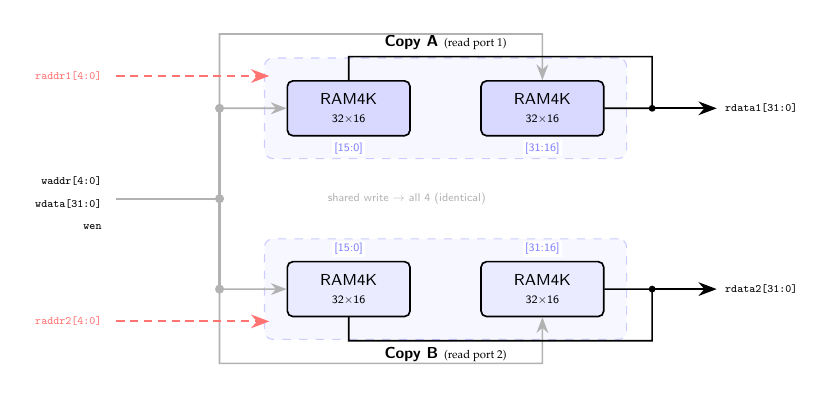
\begin{tikzpicture}[>=Stealth, semithick, scale=0.82, every node/.style={transform shape},
      blk/.style={draw, rounded corners=2pt, minimum height=0.85cm,
                  minimum width=1.9cm, font=\sffamily\scriptsize, align=center},
      arr/.style={->, thick},
      lbl/.style={font=\sffamily\tiny},
      flbl/.style={font=\sffamily\tiny, fill=white, inner sep=1pt}]

    % ---- Layout ----
    \def\by{1.4}       % Copy A y
    \def\bylo{-1.4}    % Copy B y
    \def\bL{2.0}       % left column x (low 16)
    \def\bR{5.0}       % right column x (high 16)

    % ---- 4x SB_RAM40_4K ----
    \node[blk, fill=blue!15] (a0) at (\bL, \by)   {RAM4K\\{\tiny 32$\times$16}};
    \node[blk, fill=blue!15] (a1) at (\bR, \by)   {RAM4K\\{\tiny 32$\times$16}};
    \node[blk, fill=blue!8]  (b0) at (\bL, \bylo) {RAM4K\\{\tiny 32$\times$16}};
    \node[blk, fill=blue!8]  (b1) at (\bR, \bylo) {RAM4K\\{\tiny 32$\times$16}};

    % ---- Copy boxes ----
    \begin{scope}[on background layer]
    \node[draw=blue!20, dashed, rounded corners=3pt, inner sep=8pt, fill=blue!3,
          fit=(a0)(a1), label={[font=\sffamily\scriptsize\bfseries]above:Copy A \normalfont\tiny(read port 1)}] {};
    \node[draw=blue!20, dashed, rounded corners=3pt, inner sep=8pt, fill=blue!3,
          fit=(b0)(b1), label={[font=\sffamily\scriptsize\bfseries]below:Copy B \normalfont\tiny(read port 2)}] {};
    \end{scope}

    % ---- Shared write bus (fans to ALL 4 = identical data) ----
    \node[lbl, anchor=east, align=right] at (-1.7, 0.28)  {\texttt{waddr[4:0]}};
    \node[lbl, anchor=east, align=right] at (-1.7, -0.08) {\texttt{wdata[31:0]}};
    \node[lbl, anchor=east, align=right] at (-1.7, -0.44) {\texttt{wen}};

    \draw[thick, gray!60] (-1.6, 0) -- (0, 0);
    \fill[gray!60] (0, 0) circle (2pt);
    % up to Copy A
    \draw[thick, gray!60] (0, 0) -- (0, \by);  \fill[gray!60] (0, \by) circle (2pt);
    \draw[->, gray!60] (0, \by) -- (a0.west);
    \draw[->, gray!60] (0, \by) -- (0, 2.55) -- (\bR, 2.55) -- (a1.north);
    % down to Copy B
    \draw[thick, gray!60] (0, 0) -- (0, \bylo);  \fill[gray!60] (0, \bylo) circle (2pt);
    \draw[->, gray!60] (0, \bylo) -- (b0.west);
    \draw[->, gray!60] (0, \bylo) -- (0, -2.55) -- (\bR, -2.55) -- (b1.south);
    \node[flbl, text=gray!60] at (2.9, 0.0) {shared write $\to$ all 4 (identical)};

    % ---- bit-slice labels ----
    \node[flbl, text=blue!50] at (\bL, \by-0.62)   {[15:0]};
    \node[flbl, text=blue!50] at (\bR, \by-0.62)   {[31:16]};
    \node[flbl, text=blue!50] at (\bL, \bylo+0.62)  {[15:0]};
    \node[flbl, text=blue!50] at (\bR, \bylo+0.62)  {[31:16]};

    % ---- Read addresses (one per copy) ----
    \node[lbl, anchor=east, text=red!55] at (-1.7, 1.9)  {\texttt{raddr1[4:0]}};
    \draw[arr, red!55, densely dashed] (-1.6, 1.9) -- (0.77, 1.9);
    \node[lbl, anchor=east, text=red!55] at (-1.7, -1.9) {\texttt{raddr2[4:0]}};
    \draw[arr, red!55, densely dashed] (-1.6, -1.9) -- (0.77, -1.9);

    % ---- Read data out (merge per copy, no mux: two independent ports) ----
    \draw (a0.north) -- (\bL, 2.2) -- (6.7, 2.2) -- (6.7, \by);
    \draw (a1.east) -- (6.7, \by);  \fill (6.7, \by) circle (1.5pt);
    \draw[arr] (6.7, \by) -- ++(1.0, 0) node[right, lbl] {\texttt{rdata1[31:0]}};

    \draw (b0.south) -- (\bL, -2.2) -- (6.7, -2.2) -- (6.7, \bylo);
    \draw (b1.east) -- (6.7, \bylo);  \fill (6.7, \bylo) circle (1.5pt);
    \draw[arr] (6.7, \bylo) -- ++(1.0, 0) node[right, lbl] {\texttt{rdata2[31:0]}};

    \end{tikzpicture}
    \caption{Register file mapped to EBR (\emph{synthesised} mapping --- inferred by yosys, not hand-instantiated like the SPRAM). The shared write bus (gray) writes both copies identically; \texttt{raddr1}/\texttt{raddr2} (red) drive the two independent read ports to rs1 and rs2 register indices respectively, yielding \texttt{rdata1}/\texttt{rdata2}. The two columns are the 16-bit halves of each 32-bit word; the two rows (Copy A/B) are the duplicate arrays serving the two read ports. Unlike the SPRAM banks (Figure~\ref{fig:spram-wiring}), the copies hold \emph{identical} data.}
    \label{fig:regfile-ebr}
\end{figure}

\clearpage
\subsubsection{Address decode}

PicoSoC routes each memory access purely by address: a few combinational comparisons on \texttt{mem\_addr} decide which peripheral responds --- range checks for the two memories (SPRAM and flash), exact-address matches for the config and UART registers. The selected device completes the transaction (\texttt{mem\_ready}) and, on a read, drives its data back to the CPU; if nothing matches, the CPU reads \texttt{0}. This is the standard memory-mapped-I/O decoder (Harris~\S9.2).

\paragraph{Address map.} Table~\ref{tab:picosoc-addrmap} shows the full PicoSoC address map as implemented on the iCEBreaker.

\begin{table}[htbp]
\centering\small
\renewcommand{\arraystretch}{1.15}
\begin{tabular}{@{}l l l@{}}
    \toprule
    Address range & Peripheral & Notes \\
    \midrule
    \texttt{0x03000000} & GPIO (in \texttt{icebreaker.v}) & \texttt{[7:0]}: LEDs. \texttt{[15:8]}: 7-segment display via PMOD1A. \\
    \texttt{0x02000008} & UART data register & Write: transmit byte. Read: receive byte ($-1$ if empty). \\
    \texttt{0x02000004} & UART baud divisor & \texttt{cfg\_divider} = $f_\text{clk}$ / baud $-$ 1. \\
    \texttt{0x02000000} & SPI config register & \texttt{spimemio} \texttt{cfgreg}: flash mode, latency, DDR/QSPI enable. \\
    \texttt{0x00020000}--\texttt{0x01FFFFFF} & SPI flash & Instruction fetch via \texttt{spimemio}. Reset vector at \texttt{0x00100000}. \\
    \texttt{0x00000000}--\texttt{0x0001FFFF} & SPRAM (128\,KB) & Data memory (stack, heap, globals). 4$\times$\texttt{SB\_SPRAM256KA}. \\
    \bottomrule
\end{tabular}
\caption{PicoSoC address map on the iCEBreaker (higher addresses at top). The SPRAM and flash regions are \emph{contiguous} in the low address space, partitioned at \texttt{0x00020000} ($=4\times$\texttt{MEM\_WORDS}): addresses below it go to SPRAM, addresses from \texttt{0x00020000} to \texttt{0x01FFFFFF} go to flash (the reset vector \texttt{0x00100000} lies within this range).}
\label{tab:picosoc-addrmap}
\end{table}

\paragraph{Address widths.} The CPU always issues a 32-bit \texttt{mem\_addr}. SPI Flash is byte addressed and only needs \texttt{mem\_addr[23:0]} (24 bits), because the W25Q128 chip is 16\,MB ($=2^{24}$ bytes) hence spans 24 bits. SPRAM is word-addressed: the wrapper receives \texttt{mem\_addr[23:2]} --- the byte-offset bits \texttt{[1:0]} are dropped because each access targets a full 32-bit word, with sub-word writes handled by the \texttt{wstrb} byte-enables rather than the address. Of those, only \texttt{[14:0]} (15 bits) carry information: 128\,KB is $2^{15}=32768$ words, so \texttt{addr[13:0]} indexes a bank's 16384 words and \texttt{addr[14]} selects the bank (Figure~\ref{fig:spram-wiring}). The remaining higher bits are always 0, since the decoder routes only \texttt{mem\_addr < 0x00020000} here. Hence 24 byte-address bits for a 16\,MB flash, 15 word-address bits for 32768 SPRAM words.

\subsubsection{Memory-Mapped I/O}
\label{sec:mmio}

The decode above is \textbf{memory-mapped I/O} (Harris~\S9.2): each peripheral occupies an address range and is accessed with the same \texttt{lw}/\texttt{sw} instructions as data memory --- no special I/O instructions. The textbook hardware pattern (Figure~\ref{fig:mmio-hw}) is exactly what PicoSoC builds: an address decoder driving per-device write-enables, and a read multiplexer selecting which device's data returns to the CPU.

\begin{figure}[htbp]
    \centering
    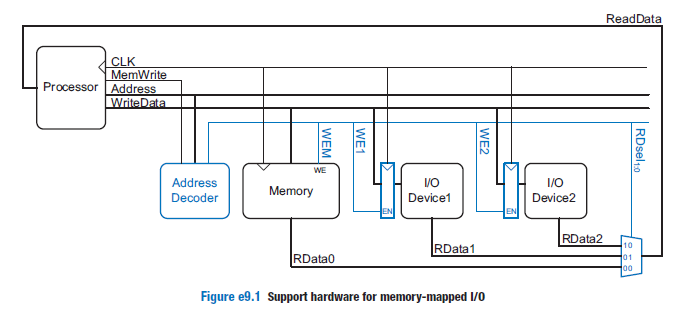
\includegraphics[width=0.5\textwidth]{figures/fige9.1.png}
    \caption{Memory-mapped I/O hardware (Harris Figure~e9.1): an address decoder generates per-device write-enables and a read-mux select. PicoSoC realises this pattern --- the address comparisons are the decoder, and the read multiplexer returns the addressed device's data.}
    \label{fig:mmio-hw}
\end{figure}

In firmware, device registers are reached through \texttt{volatile} pointers, which compile directly to \texttt{lw}/\texttt{sw}:

\begin{verbatim}
    #define GPIO_BASE  0x03000000
    #define REG_GPIO   (*(volatile uint32_t *)(GPIO_BASE))

    REG_GPIO = 0x42;                // sw: set LEDs and 7-segment display
    uint32_t val = REG_GPIO;        // lw: read back current GPIO state
\end{verbatim}

The \texttt{volatile} keyword prevents the compiler from optimising away repeated reads (e.g.\ in a polling loop).

\subsubsection{Boot sequence}

On power-up, the picorv32 begins fetching from the reset vector at \texttt{PROGADDR\_RESET} = \texttt{0x00100000} (1\,MB into flash). The startup code in \texttt{start.s} performs four steps before entering C code:

\begin{enumerate}
    \item Zero-initialise all 31 general-purpose registers (\texttt{x1}--\texttt{x31}; \texttt{x2}/\texttt{sp} is set by the \texttt{STACKADDR} parameter to the top of SPRAM).
    \item Zero-initialise the entire SPRAM scratchpad (\texttt{0x00000000} to \texttt{sp}), since SPRAM contents are undefined after configuration.
    \item Copy the \texttt{.data} section (initialised global variables) from flash to SPRAM, and zero the \texttt{.bss} section (uninitialised globals).
    \item Call \texttt{main()}. On return, an infinite \texttt{j loop} halts.
\end{enumerate}

All instructions execute from flash throughout startup (and normal operation).

\clearpage
\subsubsection{Module hierarchy}
Figure~\ref{fig:picosoc-block} shows the PicoSoC architecture with address decode logic and data return paths. The \texttt{picosoc} module instantiates the picorv32 CPU, spimemio (SPI flash controller), simpleuart, and picosoc\_mem (EBR or SPRAM). The \texttt{icebreaker} module wraps \texttt{picosoc} and adds board-specific hardware: the SPRAM wrapper, GPIO register, 7-segment display controller, SB\_IO buffers for flash, and the reset counter.

\begin{figure}[htbp]
    \centering
    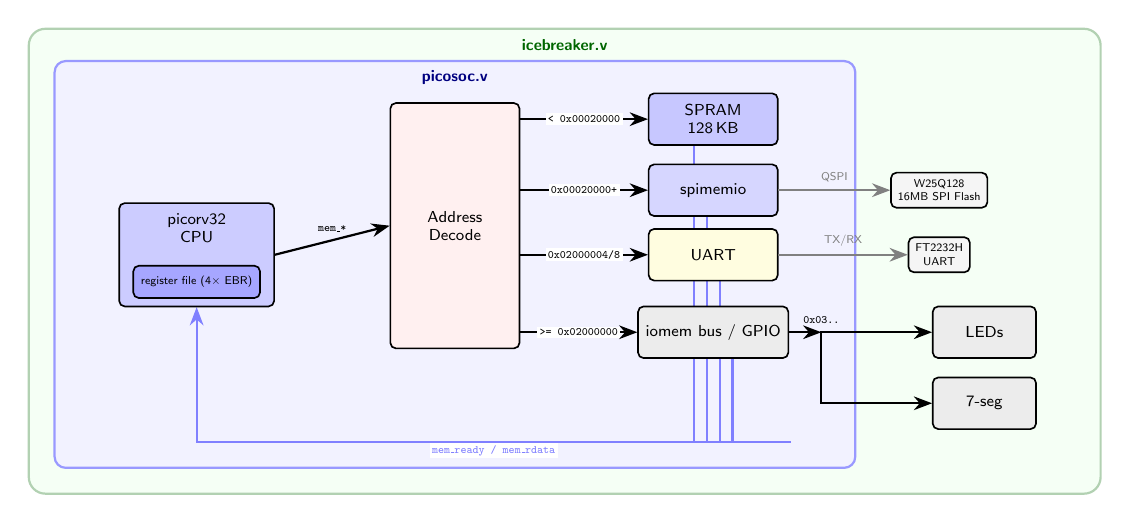
\begin{tikzpicture}[>=Stealth, semithick, scale=0.82, every node/.style={transform shape},
      blk/.style={draw, rounded corners=2pt, minimum height=0.8cm,
                  minimum width=2.0cm, font=\sffamily\scriptsize, align=center},
      arr/.style={->, thick},
      lbl/.style={font=\sffamily\tiny},
      flbl/.style={font=\sffamily\tiny, fill=white, inner sep=1pt}]

    % ============================
    % BACKGROUND: shaded boundary regions (drawn first, behind everything)
    % ============================
    \begin{scope}[on background layer]
    % icebreaker.v — outer region (green tint)
    \fill[green!4, rounded corners=6pt] (-2.6, -3.2) rectangle (14.0, 4.0);
    \draw[green!40!black!30, thick, rounded corners=6pt] (-2.6, -3.2) rectangle (14.0, 4.0);
    \node[font=\sffamily\scriptsize\bfseries, green!40!black] at (5.7, 3.75) {icebreaker.v};

    % picosoc.v — inner region (blue tint, extended left to contain return bus)
    \fill[blue!5, rounded corners=4pt] (-2.2, -2.8) rectangle (10.2, 3.5);
    \draw[blue!40, thick, rounded corners=4pt] (-2.2, -2.8) rectangle (10.2, 3.5);
    \node[font=\sffamily\scriptsize\bfseries, blue!50!black] at (4.0, 3.25) {picosoc.v};
    \end{scope}

    % ============================
    % NODES
    % ============================

    % CPU (register file nested as 4 EBR blocks --- core-internal, not on the bus)
    \node[blk, fill=blue!20, minimum height=1.6cm, minimum width=2.4cm] (cpu) at (0, 0.5) {};
    \node[font=\sffamily\scriptsize, align=center] at (0, 0.92) {picorv32\\CPU};
    \node[blk, fill=blue!35, minimum height=0.5cm, minimum width=1.9cm,
          font=\sffamily\tiny] (rf) at (0, 0.08) {register file (4$\times$ EBR)};

    % Address decoder (tall enough to span all four output lines)
    \node[blk, fill=red!6, minimum width=2.0cm, minimum height=3.8cm] (adec) at (4.0, 0.95) {Address\\Decode};

    % Memory bus: CPU -> decoder
    \draw[arr] (cpu.east) -- (adec.west)
      node[midway, above, lbl] {\texttt{mem\_*}};

    % Peripherals (stacked vertically, right of decoder)
    \node[blk, fill=blue!22] (spram)  at (8.0, 2.6) {SPRAM\\128\,KB};
    \node[blk, fill=blue!16]  (flash)  at (8.0, 1.5) {spimemio};
    \node[blk, fill=yellow!12](spicfg) at (8.0, 0.5) {UART};
    \node[blk, fill=gray!15, minimum width=2.2cm] (iomem) at (8.0, -0.7) {iomem bus / GPIO};

    % Decoder -> peripherals (with address conditions)
    \draw[arr] (adec.east |- spram)  -- (spram.west)
      node[midway, flbl] {\texttt{< 0x00020000}};
    \draw[arr] (adec.east |- flash)  -- (flash.west)
      node[midway, flbl] {\texttt{0x00020000+}};
    \draw[arr] (adec.east |- spicfg) -- (spicfg.west)
      node[midway, flbl] {\texttt{0x02000004/8}};
    \draw[arr] (adec.east |- iomem)  -- (iomem.west)
      node[midway, flbl] {\texttt{>= 0x02000000}};

    % iomem sub-decode (in icebreaker.v, outside picosoc box)
    \node[blk, fill=gray!15, minimum width=1.6cm] (gpio) at (12.2, -0.7) {LEDs};
    \node[blk, fill=gray!15, minimum width=1.6cm] (sevs) at (12.2, -1.8) {7-seg};

    \draw[arr] (iomem.east) -- ++(0.5, 0) coordinate (iofan);
    \draw[arr] (iofan) |- (gpio.west)
      node[pos=0.25, above, lbl] {\texttt{0x03..}};
    \draw[arr] (iofan) |- (sevs.west);

    % ============================
    % RETURN PATH: drawn on background layer so vertical taps go behind blocks
    % ============================
    \begin{scope}[on background layer]
    \draw[<-, thick, blue!50] (cpu.south) -- (0, -2.4) -- (9.2, -2.4)
      node[pos=0.5, below, flbl, text=blue!50] {\texttt{mem\_ready / mem\_rdata}};
    \foreach \nd/\xoff in {spram/-0.3, flash/-0.1, spicfg/0.1, iomem/0.3} {
      \draw[thick, blue!50] ([xshift=\xoff cm]\nd.south) -- ([xshift=\xoff cm]\nd.south |- 0,-2.4);
    }
    \end{scope}

    % ============================
    % EXTERNAL COMPONENTS (right edge, outside both boxes)
    % ============================
    \node[draw, rounded corners=2pt, fill=gray!8, font=\sffamily\tiny, inner sep=3pt, align=center]
      (bflash) at (11.5, 1.5) {W25Q128\\16MB SPI Flash};
    \node[draw, rounded corners=2pt, fill=gray!8, font=\sffamily\tiny, inner sep=3pt, align=center]
      (buart) at (11.5, 0.5) {FT2232H\\UART};

    \draw[arr, gray] (flash.east) -- (bflash.west) node[midway, above, lbl] {QSPI};
    \draw[arr, gray] (spicfg.east) -- (buart.west) node[midway, above, lbl] {TX/RX};

    \end{tikzpicture}
    \caption{PicoSoC block diagram. Inside \texttt{picosoc.v} (blue) the CPU's memory bus fans out by address to SPRAM, SPI flash, and the UART; \texttt{icebreaker.v} (green) wraps it and decodes the \texttt{iomem} bus (\texttt{0x03xxxxxx}) for the LEDs and 7-segment display. The register file is nested inside \texttt{picorv32} as 4 EBR blocks --- core-internal, so it carries no bus arrow (Figure~\ref{fig:regfile-ebr}). The SPI config register at \texttt{0x02000000} is not a separate peripheral: it is \texttt{spimemio}'s \texttt{cfgreg} port (flash mode/latency/QSPI). Peripherals return \texttt{mem\_ready}/\texttt{mem\_rdata} via the OR/mux chains (blue, bottom).}
    \label{fig:picosoc-block}
\end{figure}

\appendix
\begin{thebibliography}{2}

\bibitem{patterson2017}
Patterson, D.A. and Hennessy, J.L.,
\textit{Computer Organization and Design RISC-V Edition: The Hardware Software Interface},
1st ed., Morgan Kaufmann, 2017.

\bibitem{harris2022}
Harris, S.L. and Harris, D.M.,
\textit{Digital Design and Computer Architecture}, RISC-V ed.,
Morgan Kaufmann, 2022.

\end{thebibliography}

\end{document}